\documentclass[defaultstyle,10pt,master,Arial]{01.thesis}
% Helvetica is a similar font to Arial, with small differences.

%% Packages
\typeout{}
\typeout{--------------------------------------------------------------}
\typeout{ +---+ Thesis Template                            }
\typeout{ +---+      Version 2.0, August 2011                         }
\typeout{ +---+  for Instituto Superior Tecnico (IST),                 }
\typeout{ +---+  Universidade T�cnica de Lisboa                         }
\typeout{ * Using Thesis Style form Pedro Tom�s                                }
\typeout{ * Created to write Dissertations                             }
\typeout{ * Conforms with IST Master Degree format and with most important packages setup        }
\typeout{ * Should conform with IST PhD Degree format (not verified)   }
\typeout{                                                              }
\typeout{ AUTHOR: Miguel Amador and Jo�o Marques                                          }
\typeout{                                                              }
\typeout{Important: Use all files in the archive, since this is based in all them. Modify dummy files at wish.                                                              }
\typeout{--------------------------------------------------------------}
\typeout{}

\usepackage[backend=biber, style=nature, sorting=none]{biblatex}
\addbibresource{02.biblio.bib}

% Defines an additional alphabet... not required in most cases
% ------------------------------------------------------------
% \DeclareMathAlphabet{\mathpzc}{OT1}{pzc}{m}{it}

% PACKAGE babel:
% ---------------
% The 'babel' package may correct some hyphenisation issues of latex. 
% However in most situations it is not required.
\usepackage[english]{babel}
\usepackage[utf8]{inputenc}
%\usepackage[utf8, latin1]{inputenc}

% PACKAGE fontenc:
% -----------------
% chooses T1-fonts and allows correct automatic hyphenation.
%\usepackage[T1]{fontenc}
%\usepackage[latin1]{inputenc}

% Package ulem.
\usepackage{ulem} % Allows the use of other text emphatizer commands
\normalem %defines \emph{} to italic, instead of underline. 
\raggedbottom %declaration makes all pages the height of the text on that page. No extra vertical space is added. The \flushbottom declaration makes all text pages the same height, adding extra vertical space when necessary to fill out the page.

% PACKAGE date time:
% -----------------
% Lets you alter the format of the date that \today returns.
\usepackage{datetime}
\newdateformat{todaythesis}{%
\monthname[\THEMONTH]  \THEYEAR}

% PACKAGE latexsym:
% -----------------
% Defines additional latex symbols. May be required for thesis with many math symbols.
\usepackage{latexsym}

% PACKAGE amsmath, amsthm, amssymb, amsfonts:
% -------------------------------------------
% This package is typically required. Among many other things it adds the possibility
% to put symbols in bold by using \boldsymbol (not \mathbf); defines additional 
% fonts and symbols; adds the \eqref command for citing equations. I prefer the style
% "(x.xx)" for referering to an equation than to use "equation x.xx".
\usepackage{amsmath, amsthm, amssymb, amsfonts, amsbsy}
\usepackage{breqn}

% PACKAGE multirow, colortbl, longtable:
% ---------------------------------------
% These packages are most usefull for advanced tables. The first allows to join rows 
% throuhg the command \multirow which works similarly with the command \multicolumn
% The second package allows to color the table (both foreground and background)
% The third package is only required when tables extend beyond the length of one page;
% with compatibilities with the tabular environment. The last allow the definitions of landscape pages, allowing the use of a different orientation for wider graphics or tables. See package documentation to see the implementation.
\usepackage{multirow}
\usepackage{colortbl}
\usepackage{supertabular}
\usepackage{pdflscape}
%\usepackage{minipage}
% \usepackage{longtable}

% PACKAGE graphics, epsfig, subfigure, caption:
% ---------------------------------------------
% Packages for figures... well you will certainly need these packages, with the exception
% of the 'caption' package. This only allows to define extra caption options.
% Notice that subfigure allows to place figures within figures with its own caption. It
% should be avoided to create an eps file with subfigures. That will mean that you won't be 
% able to reference those subfigures. Instead create an EPS file (the only graphics format supported
% by latex) for each of the subfigures and then use the command \subfigure (see below).
\usepackage{graphics}
\usepackage{graphicx}
\usepackage{epsfig}
\usepackage[hang,small,bf]{subfigure}
%\usepackage[footnotesize,bf,center]{caption}
\usepackage{dcolumn}
\usepackage{bm}
\usepackage{booktabs}
\usepackage{rotating}
\usepackage{multirow}

\usepackage[font=small,labelfont=bf,textfont=normalfont]{caption}

% PACKAGE algorithmic, algorithm
% ------------------------------
% These packages are required if you need to describe an algorithm.
% \usepackage{algorithmic}
% \usepackage[chapter]{algorithm}

% PACKAGE natbib/cite
% -------------------
% The two packages are not compatible, and you should use one of the two. Notice however that the
% IEEE BiBTeX stylesheet is imcompatible with the natbib package. If using the IEEE format, use the 
% cite package instead
%\usepackage[square,numbers,sort&compress]{natbib}
%\usepackage{cite}

% PACKAGE acronyum
% -----------------
% This package is most useful for acronyms. The package guarantees that all acronyms definitions are 
% given at the first usage. IMPORTANT: do not use acronyms in titles/captions; otherwise the definition 
% will appear on the table of contents.
\usepackage[printonlyused]{acronym}

\usepackage{acronym} 

\usepackage[titletoc,title,header]{appendix}
\usepackage[noauto]{chappg}

% PACKAGE extra_functions VER COMO DEVE SER
% -----------------
% My Personal package: defines the following commands:
% \fancychapter{chaptername) -> Prints a fancier chapter (you can also use the fancychapter package for this)
% \hline{width} -> use for a replacement of the \hline command
% \Mark1, \Mark2, \Mark3, ...
\usepackage{00.extra_functions}


% PACKAGE hyperref
% -----------------
% Set links for references and citations in document
% Some MiKTeX distributions have faulty PDF creators in which case this package will not work correctly
% Long live Linux :D
\usepackage[plainpages=false]{hyperref}
\hypersetup{
             colorlinks=false,
             citecolor=red,
             breaklinks=true,
             bookmarksnumbered=true,
             bookmarksopen=true,
             pdftitle={Thesis Title},
             pdfauthor={Author Name},
             pdfsubject={Master Thesis in Physics Engineering},
             pdfcreator={Document Creator Name},
             pdfkeywords={Template, Latex, Thesis}}
\usepackage{float}
%\usepackage[final]{00.listofsymbols}
\usepackage{00.symlist}

% Set paragraph counter to alphanumeric mode
\renewcommand{\theparagraph}{\Alph{paragraph}~--}

\newcommand{\figref}[1]{Figure \ref{#1}}
\newcommand{\equationref}[1]{Equation (\ref{#1})}
\newcommand{\tableref}[1]{Table (\ref{#1})}

\newcommand{\textreg}{$\textsuperscript{\textregistered}$}

\usepackage{etoolbox}
\patchcmd{\thebibliography}{\chapter*}{\section*}{}{}

\usepackage{multicol}
%% Page formatting
\hoffset 0in
\voffset 0in

%Alternative set of page geometry
%\oddsidemargin 0.71cm
%\evensidemargin 0.04cm
%\marginparsep 0in
%\topmargin -0.25cm
%\textwidth 15cm
%\textheight 23.5cm

\usepackage[top=2.5cm, bottom=2.5cm, inner=2.9cm, outer=2.5cm]{geometry}

\usepackage{fancyhdr}
\pagestyle{fancy}
\renewcommand{\chaptermark}[1]{\markboth{\thechapter.\ #1}{}}
\renewcommand{\sectionmark}[1]{\markright{\thesection\ #1}}
\fancyhf{} 
%\fancyhead[LE]{\bfseries\nouppercase{\leftmark}}
%\fancyhead[RO]{\bfseries\nouppercase{\rightmark}}
\fancyfoot[LE,RO]{\bfseries\small\thepage}
\renewcommand{\headrulewidth}{0.0pt}
\renewcommand{\footrulewidth}{0.0pt}
\addtolength{\headheight}{2pt} % make space for the rule
\fancypagestyle{plain}{% Used in Chapter titles
   \fancyhead{} % get rid of headers
   \renewcommand{\headrulewidth}{0pt} % and the line
   \renewcommand{\footrulewidth}{0pt}
   \fancyfoot[LE,RO]{\bfseries\small\thepage}
}

\fancypagestyle{begin}{%
   \fancyhead{}
   \renewcommand{\headrulewidth}{0pt}
   \renewcommand{\footrulewidth}{0pt}
   \fancyfoot[LE,RO]{\bfseries\small\thepage}
}
\fancypagestyle{document}{%
	\fancyhf{} 
	\fancyhead[LE]{\bfseries\nouppercase{\leftmark}}
	\fancyhead[RO]{\bfseries\nouppercase{\rightmark}}
	\fancyfoot[LE,RO]{\bfseries\small\thepage}
	%\renewcommand{\headrulewidth}{0pt}
	%\renewcommand{\footrulewidth}{0pt}
	\addtolength{\headheight}{2pt} % make space for the rule
}
\fancypagestyle{documentsimple}{%
	\fancyhf{}
	\fancyfoot[LE,RO]{\bfseries\small\thepage}
	%\renewcommand{\headrulewidth}{0pt}
	%\renewcommand{\footrulewidth}{0pt}
	\addtolength{\headheight}{2pt} % make space for the rule
}
\setcounter{secnumdepth} {5}
\setcounter{tocdepth} {5}
\renewcommand{\thesubsubsection}{\thesubsection.\Alph{subsubsection}}

\renewcommand{\subfigtopskip}{0.3 cm}
\renewcommand{\subfigbottomskip}{0.2 cm}
\renewcommand{\subfigcapskip}{0.3 cm}
\renewcommand{\subfigcapmargin}{0.2 cm}

\graphicspath{{Figures/}}



%-----------------------------------------------------------
%-----------------------------------------------------------
\begin{document}
\pagestyle{begin}
\setcounter{page}{1} \pagenumbering{Alph}

% Add PDF bookmark 
\pdfbookmark[0]{Title}{Title}

\thispagestyle{empty}
\begin{flushleft}~\\ \vspace{-12mm} \hspace{-12mm}  
\includegraphics[width=50mm]{Figures/Cover/istnewlogo.pdf} 
\vspace{10mm}
%~\\ \vspace{50mm} % gr�ficos
\\ \begin{center} 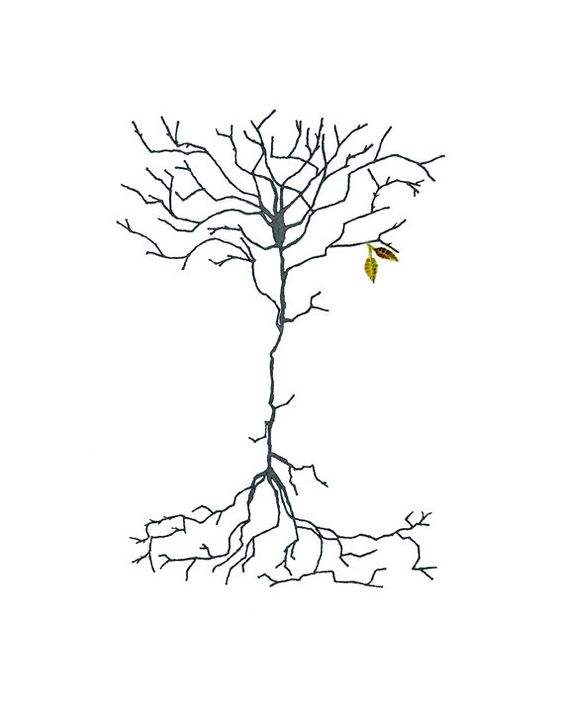
\includegraphics[height=55mm]{Figures/Cover/coverimage.jpg}  \end{center} % gr�ficos
 \vspace{5mm}
\centering
\LARGE \textbf{The spatial structure of surround modulation in mouse visual cortex}
\\ \vspace{10mm}
%\Large Subtitle
 \vspace{15mm}
\Large \textbf{Beatriz Ferreira Belbut} \\
\vspace{12mm}
\large Thesis to obtain the Master of Science Degree in
\\ \vspace{2mm}
\LARGE \textbf{Physics Engineering}
\\ \vspace{10mm}
\large Supervisors: PhD Leopoldo Petreanu and Prof. Bruno Gonçalves
\\ \vspace{15mm}
%\Large \textbf{Examination Committee}
%\\ \vspace{5mm}
%\large Chairperson:	Prof.  \\
%\large Supervisor: PhD Leopoldo Petreanu\\
%\large Co-Supervisor: Prof. Bruno Gonçalves \\
%\large Members of the Committe: Dr.  \\
%Prof. Lorem Ipsum
 
\vspace{15mm}

%\Large \textbf{\todaythesis\today} \\
\Large \textbf{October 2018} \\
\let\thepage\relax
\end{flushleft}
\pagebreak


\clearpage
% Since I am using double sided pages, the second page should be white.
% Remember that when delivering the dissertation, IST requires for the cover to appear twice.

\thispagestyle{empty}
\cleardoublepage

\setcounter{page}{1} \pagenumbering{roman}

\baselineskip 18pt % line spacing: -12pt for single spacing
                   %               -18pt for 1 1/2 spacing
                   %               -24pt for double spacingnts} 
\thispagestyle{empty}
\hbox{} \vfill
\begin{flushright}
\small \textit{\textbf{We are so familiar with seeing, that it takes a leap of imagination to realize that there are problems to be solved. But consider it. We are given tiny distorted upside-down images in the eyes, and we see separate solid objects in surrounding space. From the patterns of stimulation on the retina we perceive the world of objects and this is nothing short of a miracle.}}
\\ \vspace{2mm}  
\scriptsize Richard L. Gregory — \textit{Eye and Brain}, 1966
\end{flushright}

\clearpage
\thispagestyle{empty}
\cleardoublepage

\pdfbookmark{Acknowledgments}{Acknowledgments}
\begin{acknowledgments} 

%Leopoldo: Biology, hardware, previous software, guidance
%
%Tiago Marques: experiments, analysis, guidance
%
%Gabriela Fiorze: experiments
%
%Rhadika: Intrinsic, surgeries
%
%Oihane: Suit2p, intrinsic, surgeries
%
%Marina: surgeries
%
%Camille: surgeries
%
%Rodrigo: Tuning analysis
%
%Hedi: circuits, anatomy, connectivity
%
%all group: discussions, input, meetings, field knowledge, environment
%
%All Champalimaud comunity: CISS, posters, talks, seminars, knowledge of neuroscience
%
%Family, Francisco, friends.

\end{acknowledgments}
\clearpage
\thispagestyle{empty}
\cleardoublepage
\begin{abstract}

The Objective of this Work ... (English)

\end{abstract}
\section*{keywords}
visual neuroscience perception non-uniform asymmetry anisotropy surround modulation suppression V1 receptive field bpod spatial structure direction orientation
\clearpage
\thispagestyle{empty}
\cleardoublepage
\begin{resumo}

O objectivo

\end{resumo}
\begin{palavraschave}
Palavras-Chave
\end{palavraschave}
\clearpage
\thispagestyle{empty}
\cleardoublepage
% This is required for the fancy chapters
\dominitoc
\dominilof
\dominilot

%%%%%%%%%%%%%%%%%%%%%%%%%%%%%%%%%%%%%%%%%%%%%%%%%%%%%%%%%%%%%%%%%%%%%%
% List of contents
%\renewcommand{\baselinestretch}{1}
\pdfbookmark[0]{Index}{index}
\pdfbookmark[1]{Contents}{toc}
\tableofcontents
% \contentsline{chapter}{References}{\pageref{bib}}
\clearpage
\thispagestyle{empty}
\cleardoublepage
%\renewcommand{\baselinestretch}{1.5}
%%%%%%%%%%%%%%%%%%%%%%%%%%%%%%%%%%%%%%%%%%%%%%%%%%%%%%%%%%%%%%%%%%%%%%
% List of figures
\pdfbookmark[1]{List of Figures}{lof}
\listoffigures
\clearpage
\thispagestyle{empty}
\cleardoublepage

%%%%%%%%%%%%%%%%%%%%%%%%%%%%%%%%%%%%%%%%%%%%%%%%%%%%%%%%%%%%%%%%%%%%%%
% List of tables
\pdfbookmark[1]{List of Tables}{lot}
\listoftables
\clearpage
\thispagestyle{empty}
\cleardoublepage

% %%%%%%%%%%%%%%%%%%%%%%%%%%%%%%%%%%%%%%%%%%%%%%%%%%%%%%%%%%%%%%%%%%%%%%
% % List of algorithms
% Requires packages algorithmic, algorithm
% \pdfbookmark[1]{List of Algorithms}{loa}
% \listofalgorithms
% \cleardoublepage
\acresetall
% %%%%%%%%%%%%%%%%%%%%%%%%%%%%%%%%%%%%%%%%%%%%%%%%%%%%%%%%%%%%%%%%%%%%%%
 % List of acronyms

\pdfbookmark[1]{List of Acronyms}{loac}
%\input{acro_list}

\chapter*{Abbreviations}

\begin{acronym}[GEAI] % Give the longest label here so that the list is nicely aligned
%Note: The order matters
\acro{RF}{Receptive Field}
\acro{SM}{Surround Modulation}
\acro{V1}{primary visual cortex}
\acro{LGN}{Lateral Geniculate Nucleous}
\acro{GUI}{Graphical User Interface}
\acro{RTLSM}{Real-Time Linux State Machine}
\acro{ITI}{Inter-trial Interval}
\acro{GEAI}{Genetically Encoded neural Activity Indicator}
\acro{GECI}{Genetically Encoded Ca^{2+} Indicator}
\acro{VGCC}{Voltage-gated Ca^{2+} Channel}
\acro{ISOI}{Intrinsic Signal Optical Imaging}
\acro{TPLSM}{Two-photon Laser Scanning Microscopy}

\end{acronym}

\clearpage
\thispagestyle{empty}
\cleardoublepage




%%%%%%%%%%%%%%%%%%%%%%%%%%%%%%%%%%%%%%%%%%%%%%%%%%%%%%%%%%%%%%%%%%%%%%
% List of symbols
\pdfbookmark[1]{List of Symbols}{los}

\listofsymbols

\clearpage
\thispagestyle{empty}

\cleardoublepage
% Pages number is starting now with arabic style... until now it was on roman mode
\pagenumbering{arabic} \setcounter{page}{1}
\baselineskip 18pt
%\pagestyle{document}%Fancy head and foot with lines
\pagestyle{documentsimple}%Simple head
% %%%%%%%%%%%%%%%%%%%%%%%%%%%%%%%%%%%%%%%%%%%%%%%%%%%%%%%%%%%%%%%%%%%%%%
% The Introduction:
% %%%%%%%%%%%%%%%%%%%%%%%%%%%%%%%%%%%%%%%%%%%%%%%%%%%%%%%%%%%%%%%%%%%%%%
\fancychapter{Introduction}
\label{cap:int}

\section{A systems neuroscience question: How does the nervous system perceive the visual world?}
\label{sec:int_motivation}

Neuroscience strives to understand the organization of the nervous system, it's function and processes, as well as its relation to animal behaviour. These broad goals require a multidisciplinary integration of concepts and tools derived from biology, biophysics, anatomy, genetics, statistics, modelling, computation, ecology and psychology. Furthermore,these questions can be approached at multiple scales: from the molecular and cellular levels to the systems and neural circuits levels.

Neurons and glia, the fundamental cells in a nervous system, agglomerate in neural circuits. In the human brain, there are about $10^11$ neurons, of a great morphological and functional variety. Moreover, neurons are adaptive cells: each neurons can behave differently depending on the connections and signals it receives and transmits. 
Thus, disentangling the fundamental parameters of neuronal complexity and understanding the function of the nervous system require not only the signals and individual cell biophysical comprehension but also the understanding of the connectivity circuitry and mechanisms underlying a larger-scale neuronal network. Two systems with the same cells, arranged and interleaved with different connections would not behave equally. Correspondingly, the established knowledge on molecular and cellular neuroscience shall be integrated and complemented by a systems neuroscience approach, not as a simpler scaling step but within fundamentally different strategies. Investigating and deciphering the extraordinary questions about the nervous system in higher order completeness demand different methods, analysis and experimental paradigms than those within the study of the sum of its parts.

Neuronal systems can be described in three main functional sets: Sensory systems, motor systems and associational systems that link the former with the latter, developing more complex cognitive processes, such as perception, attention and emotions.

Animals have the enriching ability to sense the world around them. We sense our surroundings through efficiently designed stimuli sensors, and produce distinctive sensations accordingly. We are equipped with exceptionally sensible, accurate and complete input feature detectors.

However, perhaps one of the most fascinating qualities about a sensorial experience is that we can mentally encapsulate it as a given configuration and readily identify it at a future similar reoccurrence. Our nervous system allows the formation of a correspondence map between the world outside and the interior reality. The computational processing level and the efficiency of such endeavour continues to excite laborious research: How does perception arise?

In particular, the process of \textit{seeing} pertains astoundingly substantial and relevant information about the world in a remarkably efficient, fast, detailed and engaging way.

The understanding of visual perception and its processes is undertaken as one of the major withstanding challenges in systems neuroscience.

In this case, the system receives the physical image information from the retina and then parallel processes the features from the current state of the visual scene in an hierarchically organized neuronal structure. The information signals follow feedforward pathways and integrations are then carried in higher brain areas. Concurrently, feedback connections are superimposed in multiple higher order to lower order area connections, transmitting signals that underlie contextual information. Receiving this higher complexity input, neurons can then change their functioning state and produce new conjectures, educated guesses of high success probability about the input's nature. 
The unification of these parallel outputs is proposed to finally amount to a conscious sensorial perception.

There is no identity complete copy of the world outside within our perceived reality - Nonetheless, perhaps contrary to our intuition, sensitive sophisticated guesses can be just as effective, while efficient and biologically feasible within nature's parsimonious frames.

Nonetheless, fundamental questions remain for the large and complete understanding of sensory perception. In particular, discovering the computations held in the sensory cortices, their functionality, as well as the circuitry substrates that serve these mechanisms stand as main goals.

Here, we tackle a sensory neuronal property that is fundamentally implicated in visual information processing and that can yield profound insight onto the neuronal circuitry leading to visual perception - surround modulation (SM).

Neurons in the primary visual cortex (V1) respond to visual stimuli when it is presented in a given region of the visual field. For each visually responsive neuron, there is thus a \textit{receptive field} (RF) - presenting a visual stimulus of optimal parameters to that neuron in the RF corresponding visual region, will evoke a spiking response. By definition, presenting stimuli outside the RF of a neuron will amount to no response in that cell.
However, the simultaneous presentation of stimuli inside and outside the RF of a neuron will lead to a modulation of the cell's signal: the response will be either suppressed or facilitated in regards to the RF-only condition, depending on the center and surround stimuli characteristics.

This property is always active during vision processes, has been described in several species (mouse, cat, primates, humans), in various visual system areas (from the retina to the extrastriate cortex) and in multiple sensory modalities (visual, auditory, somatosensory, olfactory). A mechanistic SM theory would in this way provide a manifestly important framework in which to understand sensory processing. Moreover, understanding the circuitry that results in the SM effect and accounts for its properties can lead to insight about the function and the organization of the involved connections and network patterns - in particular, SM characterization can aid restrain circuitry models and interpret the network of inhibitory and excitatory neurons as well as feedforward, feedback and horizontal connections functionality in that perceptual integration context.

Most specifically, \textit{far} surround modulation has been suggested to require feedback input.

Typically, SM is studied in either of two methods: By using radius expanding circular grating patches or by using grating patches confined to the RF area and surrounded with annular gratings whose inner radius are made to decrease. These studies have lead to important findings about the properties of SM and elicited fruitful debate on the circuitry architectures that can result in these characteristics in a compatible way.

However, these approaches focus on static stimuli and further assume the effect's isotropy and circular symmetry. 

Recent work in mice has revealed that feedback connections from MT to V1 do not target lower-order areas irrespectively of the tuning of the higher-order sending areas. This study portrays that feedback mainly targets lower-order neurons that respond to the same positions in the visual field as the former, but that a subset of these connections are in fact dispersed to other neurons: If a higher-order neuron is tuned to a particular direction, it presents a bias to connect to a lower-order neuron that responds to the visual field positions that would appear \textit{before} in that direction line. Similarly, if a high-order neuron is orientation tuned, it presents a bias for connecting to lower-order neurons that map visual field regions at orthogonal zones to that high-order neuron's preferred orientation. 

Given the putative relation between feedback and SM, this suggested possible anisotropies in the SM effect itself, possibly to relate and to put at the perspective of the viable circuitry involved.

Here, we present an extensive characterization of SM in transgenic mice's primary visual cortex performed with two photon imaging techniques that allowed access to large datasets of differently tuned neuronal responses. We developed a moving grating stimuli presentation protocol of multiple combinations of movement directions and spatial locations that enabled the study of the spatial structure of SM and its nonuniformity.

%The mapping of moving gratings properties and the spatial structure of surround modulation can produce a set of functional rules determined in the visual cortex. It shall further provide insight into feedback mechanisms and the perception of visual scenes. 

%Precluding the project, in here we review the main related theoretical, experimental and computational topics.

%The system comprises peripheral receptors as well as central neurons. From input neurons in the retina that receive the physical image information, signals follow the visual pathway connecting to the brain, where features from the current state of the environment are parallel processed and then hierarchically repeated at higher level stages. In here, based on previously learned information of working logic inferences, the mind makes new conjectures, educated guesses of high success probability about what it is that we could be "seeing", much analogously to an extraordinarily efficient and tuned machine learning algorithm. There's no one-to-one unequivocal complete copy of the world outside within our percepted reality - But, contrary to our intuition, perhaps sensitive sophisticated guesses are just as good - as well as biologically exequivable.
%The unified binding of the parallel results of our cognition processes is presumed to amount to a conscious perception of a given state of the sensorial world.

%To investigate this complex scheme, its stages and underlying principles must be described and interpreted. 
%The purpose of this project revolves around the surround modulation effect: the finding that, if a stimulus is present in the receptive field (RF), then its surround does influence the resulting signal form of action potentials. 

%We propose the study of the spatial structure of surround modulation with motion visual scenes. This means, to analyze the effects of the location of stimuli grading patches, with varied orientations and movement directions, around the RF in the ring-shaped surround of multiple neurons of different orientation \textit{selectivity} (see section 2.2).

%Following this objective, recordings of large populations of visual cortex neurons will be obtained using two-photon microscopy in transgenic mice expressing genetically encoded calcium indicators while they observe different sets of flanking stimuli. 

%Various multidisciplinary concepts are crucial to conduct this task, and these will be motivated and exposed in the present document.

%In the following section \ref{Theoretical}, visual neuroscience main notions are described, to introduce the relevant theoretical concepts. In section \ref{Plan}, the experimental previous methods on the matter of SM are also regarded, motivating this proposal's goals and novelty. The detailed experimental procedures this project aims will then be established as to answer remaining questions about SM. This document then accounts for the relevant experimental and analytical technologies, in section \ref{Experimental}: First, an explanation is provided on behaviour measurement control settings and a programmed stimuli display protocol, as well as the further adaptations it shall undergo for this project. Secondly, the relevant principles in chemical indicators and optical physics mechanisms to use for the expression and detection of neural activity will be clarified. Finally, the analysis of the experimental data will require appropriate methods for the treatment of a large number of individual cells - We will present a possible working approach to this, Suit2p. This report will then follow with a commented bibliography, section \ref{Bib}, the calendarization of the thesis work, section \ref{Cal}, and a final discussion of the general project's plan overview, section \ref{Con}.

%\\In the following state of the art section, as a theoretical introduction, we will start by presenting visual neuroscience main general notions (section 2.1), and then specify the current understanding of the retina's neurophysiology (section 2.2) and visual cortex (section 2.3). We will then enunciate the perception organization central ideas (section 2.4) and finally review the modern surround modulation investigation results, particularizing for V1 (section 2.5).

%%other principles in neurobiology are relevant, as well as computation familiarity with Matlab, $C^{++}$, specific behavior control and measurement packages and extensions, as well as optical physics and instrumentation engineering fundaments. These will be delineated
%\\The experimental phases of this project, will be delineated starting with a section for the stimuli and software development programming (section 3.1), a review on the sort of chemical indicators, genetic manipulation and physical mechanisms used for this experiment's expression of neural activity (section 3.2) and finalized by a presentation of the recording optical technology, two-photon excitation microscopy (section 3.3).

%\\Finally, the analysis of the experimental data will require appropriate methods for the treatment of great amounts of possible parameter configurations, each for a large number of individual cells - We will present a possible working approach to this, Suit2p (section 4).

%This report will follow with a commented bibliography (section 5), the calendarization of the to-be-done work (section 6) and a final discussion of the general project's plan overview (section 7).
%\section{State of The Art}
\label{sec:int_state}

State of The Art Section.

\subsection{Dummy Subsection A}
\label{subsec:subsectiona}

State of Art Subsection A

\subsection{Dummy Subsection B}
\label{subsec:subsectionb}

State of Art Subsection B


\section{Original Contributions}
\label{sec:int_contributions}

This project can be described in two sequenced components:

\begin{itemize}
\item Stimuli display software development with bpod system for three protocols: RF mapping, tuning assessment - both adapted from the previously used bcontrol system - and SM spatial structure study. Integration of the system within the laboratory's hardware.

\item Experimental sessions with the three stimuli presentation protocols, followed by a tuning protocol validation and analytical focus on RF mapping and SM spatial structure investigations.
\end{itemize}

Within the first frame, each created protocol is made available for multiple configurations of stimuli display. The user has the flexibility to change these stimuli parameters, covering a large range of stimuli types and experimental aims.

The experimental and analytical component of the project resulted in SM spatial structure findings, for mice V1 layers 2/3. Considering that each surround patch covered a quarter-annulus around the center stimulation and that gratings could move in any of four cardinal directions:

\begin{enumerate}
\item when center and surround stimuli are simultaneously shown, there is suppression of responses in most visually responsive cells, for any stimuli configuration.
\item this suppression is significantly larger when two surround patches are displayed, instead of one (number effect).
%\item In any of the pooled conditions, going from one surround patch to two surround patches, both increased the surround 
\item there was no differential effect of SM with left versus right surround patches. The data was not conclusive for a top versus bottom surround patches effect (position effect).
\item there was a significant effect of increased suppression with shorter distances from the RF center to the surround stimuli, in the horizontal axis of the display, even whilst the cells did not respond to any of the surround-only conditions (distance effect).
\item suppression was weakly but significantly stronger for surround gratings going in the temporal direction versus going in the nasal direction. No significant difference was found for SM strength with surround gratings going in up versus down directions (direction effects).
\item Comparing surround gratings moving horizontally versus vertically held a slight but significant difference, with horizontal gratings' orientation corresponding to stronger suppression than vertical orientation (orientation effect).
\item suppression is significantly stronger when surround stimuli is presented in positions collinear to its direction of movement than when presented in flanking positions regarding that direction (alignment effect).
\item suppression is significantly stronger when presenting surround stimuli iso-directed to the center stimulus direction than when showing it cross-directed to the center stimulus direction (angle effect).
\item comparing responses from orientation selective neurons (OS), when the stimuli presented in the center was either colinear, flanking, iso-directed or cross-directed but in the preferred direction versus when in was in the anti-preferred direction yielded that suppression was significantly weaker for the former, plus the alignment and angle effects were larger. 
\item significant interactions were found between the number effect and the alignment effect, between the number effect and the angle effect and between the alignment effect and the angle effect. 
\item the variances found in the distributions of SM strength were, by quantitative order, attributable to the number effect, the preference effect, the alignment effect and the angle effect.
\end{enumerate}

In addition to these, the obtained data portrayed other trends which did not prove statistically significant. Additional data is required to discard or validate those hypothesis:

\begin{itemize}
\item surround stimuli moving towards the center stimuli versus outwards: data shows a barely significant effect for stronger suppression with the former.
\item surround stimuli and center stimuli moving in convergent versus divergent directions: data does not hold significance.
\item two surround patches moving in the same versus opposite directions to the center direction: data does not hold significance.
\end{itemize}
\section{Thesis Outline}
\label{sec:int_outline}

In the following section \ref{cap:TheoreticalIntroduction}, visual neuroscience main state of the art notions are described, to introduce the relevant theoretical concepts. 

In the technology chapter \ref{cap:Technology}, we review the chemical indicators, genetic manipulation and physical mechanisms used for this experiment's expression of neural activity, as well as the recording optical technologies, namely intrinsic signal optical imaging and two-photon excitation laser-scanning microscopy.

Chapter \ref{cap:TechnicalImplementations} describes and explains the software development phase and implemented system for stimuli display, elucidating the technical outcomes of the project.

Chapter \ref{cap:ExperimentalMethods} details the experimental methods, starting with the procedures performed with the animals, following with the visual stimulation setups for both intrinsic imaging and two-photon microscopy, then describing the experimental sessions' pipelines, stimuli presentation structure and stimuli parameters for the three protocols (RF, tuning and SM spatial structure study).

The analysis of the experimental data required appropriate methods for the treatment of great amounts of possible parameter configurations, each for a large number of individual cells. In chapter \ref{cap:Analysis}, first we enunciate the raw outputs of an experimental session and follow with the preliminary image processing stages applied to the recorded imaging data - plane separation and registration. Suit2p pipeline is then presented, as it was used for semi-automated selection of regions of interest (ROIs) to regard as neurons. Finalizing the general data treatment stages, normalized fluorescence extraction is explained. After these points, we follow with the specific analysis methods for each protocol. To conclude the chapter, we present a review on statistical notions applied for the SM data comparison analysis.

This project's results are then described in chapter \ref{cap:Results}. We start with the intrinsic optical imaging maps, follow with the general RF mapping results, tuning properties assessment and finish with the SM results analysis of individual example cells and a broader population study for SM effects.

Finally, a discussion on the findings follows in chapter \ref{cap:Discussion}, integrating the previously established SM properties across species and sensory areas with those hereby presented and contextualizing this project's results within the SM current theories. We conclude with an overall review of the project's process and enumerate potential related future work.

%In section \ref{Plan}, the experimental previous methods on the matter of SM are also regarded, motivating this proposal's goals and novelty. 

%The detailed experimental procedures this project aims will then be established as to answer remaining questions about SM. This document then accounts for the relevant experimental and analytical technologies, in section \ref{Experimental}: First, an explanation is provided on behaviour measurement control settings and a programmed stimuli display protocol, as well as the further adaptations it shall undergo for this project. Secondly, the relevant principles in chemical indicators and optical physics mechanisms to use for the expression and detection of neural activity will be clarified. Finally, the analysis of the experimental data will require appropriate methods for the treatment of a large number of individual cells - We will present a possible working approach to this, Suit2p. This report will then follow with a commented bibliography, section \ref{Bib}, the calendarization of the thesis work, section \ref{Cal}, and a final discussion of the general project's plan overview, section \ref{Con}.

%\\In the following state of the art section, as a theoretical introduction, we will start by presenting visual neuroscience main general notions (section 2.1), and then specify the current understanding of the retina's neurophysiology (section 2.2) and visual cortex (section 2.3). We will then enunciate the perception organization central ideas (section 2.4) and finally review the modern surround modulation investigation results, particularizing for V1 (section 2.5).

%%other principles in neurobiology are relevant, as well as computation familiarity with Matlab, $C^{++}$, specific behavior control and measurement packages and extensions, as well as optical physics and instrumentation engineering fundaments. These will be delineated
%\\The experimental phases of this project, will be delineated starting with a section for the stimuli and software development programming (section 3.1), a review on the sort of chemical indicators, genetic manipulation and physical mechanisms used for this experiment's expression of neural activity (section 3.2) and finalized by a presentation of the recording optical technology, two-photon excitation microscopy (section 3.3).

%\\Finally, the analysis of the experimental data will require appropriate methods for the treatment of great amounts of possible parameter configurations, each for a large number of individual cells - We will present a possible working approach to this, Suit2p (section 4).

%This report will follow with a commented bibliography (section 5), the calendarization of the to-be-done work (section 6) and a final discussion of the general project's plan overview (section 7).

\cleardoublepage
% %%%%%%%%%%%%%%%%%%%%%%%%%%%%%%%%%%%%%%%%%%%%%%%%%%%%%%%%%%%%%%%%%%%%%%
% Dummy Chapter:
% %%%%%%%%%%%%%%%%%%%%%%%%%%%%%%%%%%%%%%%%%%%%%%%%%%%%%%%%%%%%%%%%%%%%%%

% %%%%%%%%%%%%%%%%%%%%%%%%%%%%%%%%%%%%%%%%%%%%%%%%%%%%%%%%%%%%%%%%%%%%%%
% The Introduction:
% %%%%%%%%%%%%%%%%%%%%%%%%%%%%%%%%%%%%%%%%%%%%%%%%%%%%%%%%%%%%%%%%%%%%%%
\chapter{Theoretical Introduction}
\label{cap:TheoreticalIntroduction}

\textit{Present the chapter content.}

%\section{Visual Neuroscience: Perception}
\label{sec:sectiona}

\section{Brain visual pathways}
\label{sec:sectionb}

\subsection{The eye}

Most of the visual relevant information we receive consists of spatial and time variations in light intensity. When receiving light, the retina maps the light's temporal and spatial patterns onto a layer of receptor cells that respond to light with an electrical activity pattern in a retinotopical map: organized, topographically ordered representations of the visual field.  

The retina is the innermost layer of the eye, and a part of the central nervous system. It contains light-sensitive neurons, photoreceptors, and allows for the transmission of visual signals through another class of neurons, the ganglion cells. It also contains horizontal, bipolar and amacrine cells. Horizontal and amacrine cells mediate lateral interactions. The major route of information in the retina follows from the photoreceptors to the bipolar cells and finally to the ganglion cells. Each ganglion cell responds by changing its firing rate to stimulation of a roughly circular concentric patch of the retina, its classical \textit{receptive field} \cite{Kuffler1953}. This information is then relayed to the brain.

The photoreceptors, rods and cons, are the first intervenients, and account respectively to the sensitivity and the acuity in the detection of light.
When light falls in the retina's photoreceptors, they are activated by means of grated changes in membrane potentials that then induce corresponding changes in the rate of synaptic transmitter release from ganglion cells. 

To allow the eye to respond efficiently over great spatial and temporal ranges in illumination intensity, this regulation's criteria is based on judicious input's pattern transformations. Both the temporal and spatial conversions code information by means of giving prominence to rapid \textit{changes} and filtering out slow changes in light intensity over time and space.

The temporal frequency in the photoreceptors undergoes \textit{adaptation} - with major impulse rate signals corresponding to a sudden peak in light intensity that is rapidly set back to a lower steady level. The ganglion cell's response rates depend as well on the background level of illumination, with adaptive range shifts that scale the response to a visual scene's illumination levels. In this way, the retina normalizes the received inputs in relation to the full image's statistics. 

Concerning the spatial pattern, the question becomes, how are the different receptors responses jointly treated? In fact, \textit{lateral inhibition} arises: If, while in the dark, a small light stimulus appears, rod cell's will be enhanced. The rod cells corresponding to the center of the stimulus' location will send an activated signal. However, due to lateral inhibition from horizontal cells, the different rod cells outside the stimulus' location will send an inhibitory signal. This implies the prominence of boundaries between bright and dimmed regions.

Both the temporal and spatial transformations code information by means of giving prominence to rapid \textit{changes} and filtering out slow changes in light intensity over time and space. 

The sensitivity to light-dark borders in the visual scene is further achieved by the two ganglion cells classes, on-center and off-center. These cells are sensitive to differences between illumination levels in its receptive field center and in its ring-shaped surround. In an on-center ganglion cell, brightly illuminating a central spot of the receptive field produces a burst of action potentials. In an off-center cell, the response to the same stimulus is a reduced rate of action potentials, and an increase as the illumination is turned off. The responses are the complementary in the case of introducing dark spots. In this way, there are two separate channels of luminance \textit{changes} information being carried to the brain, and either increases or decreases in brightness are always encoded as increased action potentials in the ganglion cells.


%Chapter 3 in 'visual perception', Visual pathways in the brain

%Kandel Principles of Neural Science Book

%Purves Neuroscience Book


\subsection{Central Visual Pathways}

Firstly, the primary visual pathway mediates vision and visual perception. Information is driven from the retina, to the thalamic dorsal lateral geniculate nucleus (LGN) and finally to the primary visual cortex (V1).%, all containing different kinds of neurons for encoding various visual properties.

Ganglion cell's axons follow a path over the retina's surface to the optic disk, bundling together in the optic nerve. %This retina's region is insensitive to light and is therefore responsible for the blind spot - a substancial gap in each monocular visual field. 
From here, the ganglionic axons continue to the optic chiasm, past which the axons from both sides form the optic tract. These axons then continue to the brain, mainly projecting in the dorsal lateral geniculate nucleous (LGN) in the thalamus. The LGN is arranged in layers and appears in both brain hemispheres,  receiving information from the left and right semifields of view detected by each of the two retinas. These then radiate to the striate cortex, in the primary visual cortex V1, mostly to layer 4 (out of 6 functionally distinct ones).

The ganglion cells can also project to the pretectum, an area that treats reflex control of the pupils and lens. Other targets comprise the suprachiasm nucleus of the hypothalamus, controlling the visceral night/day cycle functions and the superior colliculus that coordinates head and eye movement. Each of this routes requires different types of visual information, in terms of its resolution, features detail and properties' measurements. 

In both LGN and V1, the retinotopy is mantained.
As with the retina cells, visual neurons can be described in terms of their receptive field: the visual field area to which the neuron evokes a spiking response when a isolated local stimulus of optimal parameters is presented in that region \cite{Hubel1959}.

In accounts for these cells stimulus response organization, the LGN cell's receptive fields are concentric and ruled analogously to those from the ganglion cells. 
However, the striate cortex's V1 cells can have different organizations of their receptive fields, with different distributions and numbers of excitatory and inhibitory areas. 

Furthermore, neurons in the striate cortex have an added property: they can be tuned, and present selectivity to particular features. A neuron's tuning can be specified for any stimuli space, and its responsiveness measured for different points within that space. 

Foremost, the response of neurons in cortical areas such as V1 is found to be tuned to orientation of edges. The orientation to which a given cell produces the larger response is called the preferred orientation of the neuron, and all orientations are equally represented in the visual cortex. For cats and primates, V1 neurons are mostly organized in columns of different selectivity to particular stimuli attributes: Across layers, in the same direction, neurons respond to the same orientation. Hence, receptive fields are repeatedly represented into modular sheets of neuron distributions in each sublayer. Furthermore, some cortical neurons are selective to lengths or to the direction of stimuli bars, to color, spatial frequency or ocular preference - relative strength of the input from the two eyes. 

Following from V1, extrastriate cortical areas are organized into two large systems: The ventral stream, following V1 to V2 to V4 and connecting to the temporal lobe, thought to account for object recognition, high-resolution images treatment; and the dorsal stream, with a path from V1 to V2 to MT and connecting to the parietal lobe, thought to process the analysis of motion and positional relations between objects in a visual image, as well as attention control. Accordingly, neurons in the ventral stream are selectively tuned to shape, color, texture and, in higher levels, to faces and objects. It is however important to note that, for example, a given specific face's recognition is encoded by a specific pattern of activity in a population of cells, and not by the unique firing of a super-narrowly specific cell. On the other side, dorsal stream's neurons are selective to elements such as movement's direction and speed, containing a detailed map of the visual field.

Neurons at higher levels in the visual pathway are increasingly tuned, latent, and in general have larger receptive fields.

Ascending away from the striate cortex, an hierarchy can be recognized, evolving from the analysis of simple attributes of an image, such as contrast, colour, orientation of segments, going to intermediate level vision, regarding contour integration and surface segmentation, and finally turning to more complex visual processings such as object recognition. 


\subsection{Feedforward: spatial filtering of natural images}

Ganglion cells can be treated as low-pass spatial filters, producing responses to sinusoidal gratings having a variety of spatial frequencies, with a given range (the neuron's bandwidth) determined by the receptive field's size. 

The neuron's bandwidth becomes narrower as we go from ganglion to LGN and then to striate cortex cells. 

Particularly, simple cells can, in this sense, be described as Gabor functions \cite{Jones1987}, a product of a sine function and a gaussian envelope. This description accounts for the necessary trade-off in spatial frequency and spatial location specificity: A wider gaussian relates to a wider receptive field and thus a narrower spatial frequency bandwidth, but a larger set of possible stimulating spatial locations. This motivates the idea for the efficient encoding strategy of the natural visual world. In a given image, redundancy is expected: it is probable that the light reaching one photoreceptor will be strongly correlated to the light that reaches its neighbours, and thus, at first levels such as V1, high specificity is not required, and patterns can be more economically encoded.

On the other hand, striate cells can be regarded as bandpass filters, with a greater variation in the allowed spatial frequency tuning. 
The striate cortex processes many differently located patches from the retinal image, each containing different spatial frequencies, with the firing rate of each cell accounting for the amplitude of the frequency component to which the cell is tuned - a patch-wise Fourier analysis of the input image.


\subsection{Feedback pathways and influences}

Up until this point, this description has focused on the classical model of feedforward transmission of sensory information in an hierarchy of cortical visual areas, beginning with V1 and following through the ventral and the dorsal pathways.
However, visual pathways are bidirectional. Superimposed in these bottom-up connections, there are reentrant pathways that transmit influences in the reversed top-down direction, in every stage of the visual pathways except for the retina, from higher order cortical areas to neurons in lower processing levels.

To understand these reciprocal interacting mechanisms that can cause non-linear effects, another point must be made explicit: Neurons do not function as fixed functional processors, but rather as adaptive units that can change their function depending on the behavioral context, subject to attention, expectation and perceptual task instructions, at any given processing moment.

This adaptation appears via both changing of neurons' tunings to stimuli - changing of their receptive fields characteristics - and by alteration of the correlations structure of neuronal ensembles.

The neuron changes its \textit{line label}, in accordance to higher orders instructions: A neuron's response means that a stimulus with its preferred attributes is being detected, being the signal as strong as the stimulus is close to that preferred configuration. However, accounting for feedback, a cell can function in different functional states and the meaning of the information they convey depends on that state - its preferences are changed. The analysis is not misinterpreted because the higher areas that send the adaptative instruction to a given neuron or population of neurons also treat the resulting returning signal.

On the other hand, a network of neurons within the same, as well as across different cortical areas, can change their spatial and temporal distribution of correlated activity. In fact, if neurons can be made independent to one another, an ensemble of such neurons will have less variability than that of a single neuron's response to a given stimulus, allowing for better signal to noise ratios of that process and thus for more optimal information encoding.

Vision is then seen as an active process, with feedback conveying signals that adapt the lower neurons in such a way that allows them to encode more relevant information within a given contextual paradigm, facilitating the visual scene representation and interpretation: Their responses to a stimulus are made more informative about the identity of that stimulus. Moreover, given the complexity of the neural pathways, this idea implies that any given cell receives input, directly or indirectly, through feedforward or feedback entrances, from each other relevant processing stage, in a way representing the full brain on their own.

%Beyond a straightforward low-level analysis of simple local attributes, under feedback influences, neurons can integrate six main different forms of contextual information: Spatial, object and feature oriented attention; the at hand perceptual task; object expectation; another behavioural context effect is the case of eye movement across a visual scene. For the image to continue appearing stable, an efference copy of the motor instruction for the eye movement is kept in higher cortical levels and this information is then sent to the retina that compensates for that signal; Finally, top-down influences can also provide memorized and learned information. 

Beyond a straightforward low-level analysis of simple local attributes, under feedback influences, neurons can integrate six main different forms of contextual information: firstly, spatial attention can enhance some responses and suppress others outside the attention focus, facilitating the selection of behaviourly relevant stimuli from distracters. second, the discriminability of features of the same object - object oriented attention - and components with similar characteristics - feature oriented attention - can as well be enhanced. The neurons' tuning can also change according to the perceptual task at hand, allowing for the discarding of irrelevant stimuli information to the considered task. Object expectation can also play a feedback role, when a subject is cued to seek for a specific shape.  Finally, top-down influences can also come as working memory, associative memory and perceptual learning information, with prior experience at shorter and longer term yielding important processing instructions. 

Feedback thus enables neurons to process information from contextual influences, relating to larger parts of the visual field and these can as well become selective to more global visual scene configurations. Moreover, feedback has also been implicated in making each neuron's response more relevant, more informative and sparse in the individual's context.

%Feedback: Some forms of these signals appear as predictive hypothesis testings, as higher-levels predict an image from the lower-level activity, and this is carried back with an error signal between the prediction and the stimulus-based signal.


\section{Surround modulation in the visual cortex}

Thought to underlie optimal coding efficiency, sensory processing and perception, sensory neurons exhibit the surround modulation phenomenon: 

A stimulus inside a neuron's RF will produce a response of activation in a small part of the visual field. While the same stimulus will not activate the neuron if it is represented outside its RF, if jointly presented in both regions, a modulation of the neuron's signal will take place. This facilitatory or inhibitory modulation will depend on the relative stimuli characteristics in both locations. 

This property was initially found in cat V1 (\cite{Hubel1965}), and has currently been shown to occur in many species - mouse (\cite{Bergh2010}), cat (\cite{Blakemore1972}), monkey (\cite{Cavanaugh2002a}); in humans, spatial context has been shown to alter the perception of a visual target (for example, \cite{Chubb1989}, \cite{Cannon1991}, \cite{Meese2004}, \cite{Nurminen2009}) -, sensorial systems and processing levels, ranging, for the visual system, from the retina (\cite{McIlwain1964}, \cite{Solomon2006}) to neurons in the extrastriate cortex (\cite{Allman1985}, \cite{Desimone1987}, \cite{Born2005}). 

It has been particularly studied in the visual system, area V1 (\cite{Hubel1965}, \cite{Blakemore1972}, \cite{Maffei1976}, \cite{Gilbert1977}, \cite{Nelson1978}, \cite{Sceniak2001}, \cite{Cavanaugh2002a}, \cite{Bergh2010}, \cite{Angelucci2013}; for a review, \cite{Angelucci2017}).

Typically, visual SM is studied with either of two methods: An expanding circular grating patch, or RF grating patches surrounded by gratings in an annulus, whose gratings parameters are made vary sistematically (for a review, \cite{Angelucci2014}).

Summarily, SM in V1 has been described with five main attributes: 

First, it is spatially extensive, with SM strength decreasing with distance from the neuron's RF (\cite{Sceniak2001}, \cite{Cavanaugh2002a}, \cite{Levitt2002}, \cite{Shushruth2009});

Secondly, SM effect's sign and strength are also dependent on the strength of stimuli activation in both the RF and the surround - stimulus size, orientation optimality and contrast levels. In fact, when the RF is strongly stimulated (high contrast, optimal orientation and size stimulus), either weakly (low contrast or suboptimal orientation or size stimulus) or strongly activated surrounds will cause a suppressive effect. Conversely, when the RF is weakly activated, strongly activated surrounds will also evoke suppression, but weakly activated surrounds can lead to facilitatory modulation (\cite{Polat1998}, \cite{Chen2001}, \cite{Ichida2007}, \cite{Shushruth2012}).

Moreover, SM is fast, and can be described in two temporal components: The earliest is untuned to the stimulus properties and can occur at the onset of the RF response with no delay (\cite{Muller2003}, \cite{Henry2013}), nearly independently from the distance of the surround stimulus (\cite{Bair2003}). The later component is tuned and $10-30 ms$ delayed in relation to the onset of RF responses (\cite{Bair2003}).

Additionally, SM properties are different across cortical layers: In layer 4C that does not receive feedback relay, but inputs from the LGN, SM is weaker, untuned for orientation and less spatially expansive than for any other layer. On the other hand, for more superficial layers 4B and above, SM is stronger and more sharply tuned for orientation than for the deeper layers.

Finally and most importantly, SM is tuned to specific stimulus parameters, suppressing more strongly responses for stimuli in the RF and surround with the same orientation, spatial frequency, drift direction and speed and either weekly suppressing or even enhancing the signals for orthogonal parameters (\cite{deAngelis1994}, \cite{Li1994}, \cite{Sengpiel1997}, \cite{Walker1999}, \cite{Cavanaugh2002a}, \cite{Muller2003}, \cite{Webb2005}, \cite{Henry2013}, \cite{Self2014}). This differentiated effect appears even if the RF stimulus is not at the neuron's preferred orientation: the stronger suppression for iso-oriented stimuli is present provided that the RF stimulus evokes a response when presented alone, even if this is not the maximal response.

SM has been implicated with a variety of possible visual processes and functions.

From its property of evoking stronger responses for dissimilar stimuli inside and outside a neuron's RF, SM can evoke visual saliency (\cite{Knierim1992}), perception of object boundaries (\cite{Nothdurft2000}), and figure-ground segregation (\cite{Lamme1995}), by enhancing neuronal responses in discontinuity areas.

Secondly, another reported SM effect is that small collinearly aligned line segments with the same orientation can lead to facilitated responses. This suggests a SM function for contour integration, aiding in the detection of discontinuous lines from a background of lines with other orientations (\cite{Kapadia1995}, \cite{Polat1998}, \cite{Field2013}).

Furthermore, SM functional role could also be to reduce redundancies in neuronal responses and increase response sparseness (this SM result was experimentally shown in \cite{Vinje2000}, \cite{Wolf2014}, \cite{Pecka2014}), making the full neuronal system more efficient (\cite{Barlow1961}). For instance, the finding that similarly oriented lines in the RF and the surround produce a suppressed signal can be intuited in the light that neighbour lines with the same inclination are statistically expected in a natural image and thus don't require a prominent encoding. SM would thus serve to reduce the spatial and temporal correlations from the visual world to the neuronal representations.

Another implication from SM properties, is that RF size will be larger when it is measured for low contrast than when it is measured for high contrast levels (\cite{Sengpiel1997}, \cite{Sceniak1999}), when RF size is measured with the gratings expanding method, as the summation RF that determines the RF size as the corresponding size of the stimulus displayed at the point when the evoked neuronal activity starts decreasing (see figure \ref{SMcontrast} response curves depiction). Therefore, RF definitions can be made, with $sRF_{high}$ and $sRF_{low}$, respectively the summation RF measurements at high and low contrast levels. Visual stimulation between these two summation RF sizes will cause suppression at high contrast and facilitation at low contrast. One can then define this the near-surround region and term the region beyond it the far-surround (\cite{Angelucci2017}).

\begin{figure}[H]
\center
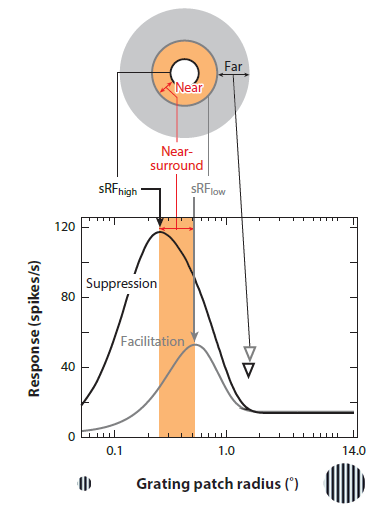
\includegraphics[scale=0.8]{2.Chapter/SMcontrast.png}
\caption{Response curves of a cell in V1 to high-contrast (black curve) and low-contrast (gray curve) as a function of the radius of displayed grating patch stimuli. The point of highest response at high-contrast is termed $sRF_{high}$ and the peak's corresponding size at low-contrast is termed $sRF_{low}$. The near surround is depicted in orange and the far surround in gray. Suppression arises in the near-surround and far-surround for high-contrast stimulation and on the other hand facilitation is evoked in the near surround and suppression in the far-surround for low-contrast gratings.
\newline \newline \tiny{Image from \cite{Angelucci2017}, adapted from experimental data tuning curves for macaque V1 in \cite{Shushruth2009}, at different contrast levels.}}
\label{SMcontrast}
\end{figure}

In this way, V1 SM has been proposed to consist on these two different components, arising from different anatomical circuits, having different tuning and spatio-temporal properties and possibly amounting to different functional perception roles (\cite{Nurminen2014}). Near-SM is more strongly suppressive (\cite{Shushruth2009}) and more sharply tuned to orientation than far-SM. In humans, these orientation perception differences are also found similar in perceived contrast for near-surround and far-surround modulation (\cite{Shushruth2013}). These different circuits can aid an efficient encoding of natural scenes (\cite{Sushruth2013}). In the world, it is more statistically probable for nearby edges to belong to the same object contour if these are iso-oriented. By suppressing evoked responses for this high-occurrence contours, dependencies are minimized by tuned near-SM and the neuronal encoding is made more sparse. Moreover, decreased SM for cross-oriented lines in the near visual field can aid in object boundaries segmentation. On the other hand, for far away edges in natural scenes, statistical dependencies decrease with distance and also become less orientation dependent. Moreover, observers are more likely to perceive that two nearby edges belong to the same contour if these have the same orientation, but for far edges a wider range of orientations is possible (\cite{Wertheimer1958}). Far-SM shows similar distance-dependence properties (\cite{Nurminen2014}). Far-SM suppresses irrespectively of the orientation differences between edges, except when this orientation difference is very marked. This effect can thus lead to enhancement of the responses for salient distant edges, guiding saccadic eye movements and the subject's attention \cite{Petrov2006}.

Regarding the circuits connections implicated with each SM component, feedforward projections from the LGN, long-range intra-V1 horizontal connections and extra-striate feedback have all been implicated. A proposal (\cite{Angelucci2002}, \cite{Angelucci2006}, \cite{Nurminem2014}) attributes these feedforward and horizontal connections to the near-surround and feedback to the far-surround (image \ref{SMcomponents}).

\begin{figure}[H]
\center
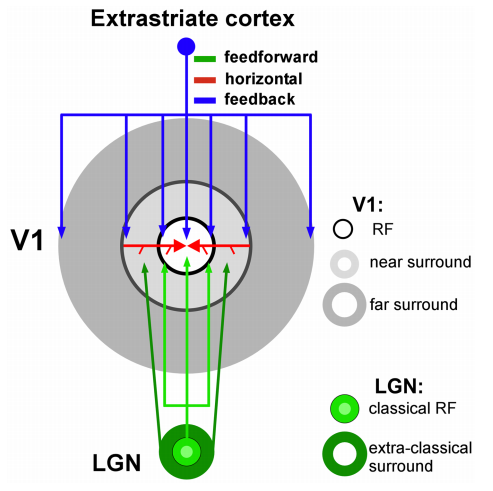
\includegraphics[scale=0.8]{2.Chapter/SMconnections.png}
\caption{The near and far components of SM and its hypothesized underlying circuits and functions. Coloured arrows indicate the different connections proposed to generate the different areas of V1 neurons - RF, near and far surround. In color code, the major functional possible roles of each connection type and surround component are presented.
\newline \newline \tiny{Image from \cite{Shushruth2013}.}}
\label{SMconnections}
\end{figure}

Feedforward contributions to SM are primarily in regards to adapting the size and tuning properties of V1 neurons (\cite{Hubel1962}, \cite{Angelucci2006}). This feedforward component to SM is fast, broadly tuned for orientation and confined to the near-surround. This component's function is suggested to be in normalizing V1 neurons' responses in regards to stimulus contrast. This is a computation found in V1 (\cite{Heeger1992} that enables neurons to process wide ranges of contrast stimuli in visual scenes, despite the neurons saturation limitations (\cite{Carandini2012}). There is however also evidence for a cortical contribution to untuned suppression. For example, modeling work has shown that long-range tuned suppression from horizontal connections interacting with local untuned suppression steaming from feedforward suppression effects causes SM to become tuned to the stimulus orientation presented to the cell's RF and not the cell's preferred orientation (\cite{Shushruth2012}), as established from the experimental evidence for this SM property (see above, V1 SM fourth property).

Horizontal connections in V1 are most prominent in layers 2/3, come from excitatory neurons and target both excitatory and inhibitory neurons of similar orientation selectivity (\cite{Bosking1997}, \cite{Malach1993}, \cite{Schmidt1997}, \cite{Sincich2001}). This is then thought to underlie near SM tuned component (\cite{Gilbert1996}). This component is proposed to be involved in the efficient encoding sparseness strategy functions of SM, aiding in object segmentation.

Finally, extrastriate feedback relays arise from excitatory neurons in layers 2/3 and 5/6 and project to both excitatory and inhibitory neurons (\cite{Anderson2009}). These connections are spatially spread, and can cover the extensive far-surround modulation to V1 neurons (\cite{Angelucci2002}). Feedback from different areas is fast, with connections at high conduction velocities (\cite{Girard2001}) and can convey information from visual field regions 5 to 25 times larger than the RF size. These properties are well suited to mediate far-SM. Moreover, recent research (\cite{Nurminem2018}) has shown with specific optogenetic inactivation of feedback connections, that decreasing feedback activity increases V1 neuron's RF size, decreases their responses to stimuli in the RF and increases responses to stimuli on the surround, thus decreasing surround suppression. Feedback functional organization is not known. Feedback has however been implicated with attention \ref{subsec:feedback}, as spatial attention also increases neuron's responses at attended sites (\cite{McAdams2005}), modulates surrond suppression (\cite{Sundberg2009}) and RF size (\cite{Roberts2007}). If indeed it mediates far-SM, its properties could amount to visual salience in dissimilar stimuli at far distances, as well as the directing of saccades and attention functions. 

A working hypothesis \cite{Schwabe2006} builds on experimental proposals and biological plausability (\cite{Angelucci2017} for an evaluation of the model against available data) that SM can come from complex interactions of feedback, feedforward and horizontal connections, and implements an architecture both with increased inhibition, strong recurrency and balanced recurrent inhibition and excitation of signals (\cite{Shushruth2012}). The computational model accounts for both the tuned and untuned components of SM, and works with surround stimulation activating both horizontal and feedback connections that then modulate V1's center-encoding local recurrent network, via excitatory contacts to both excitatory and two types of inhibitory neurons, one of which is tuned for orientation (contacting back excitatory only if those are in the same orientation preference) and the other which is untuned for orientation. Adapted for novel data and parameter-restricted for fitting with recent findings, recurrent network models can be paramount to fully describe SM, as the non-linearity of these networks, beyond a simple feedforward ordered network, may exhibit complex behaviour that can only be explained and intuited at the appropriate non-linear paradigm.

Nevertheless, great debate is still conducted on the mechanisms that can cause SM, as well as on the circuits that mediate it. Furthermore, the functional roles of feedback are yet to be fully described, differentiated between brain areas and related to possibly separated or interacting SM effects. Finally, finding and explaining the canonical stimuli properties and components that SM effects are dependent on can entail a greater fundamental understanding of the phenomenon and its underlying networks. 

\subsection{SM non-uniformity}
%\section{Receptive fields and tuning}
\label{sec:sectionb}

%\section{Feedback as a path for contextual information integration}
\label{sec:sectionb}


\section{The motivation: feedback organization rules - uncovering the functions of feedback}
\label{subsec:subcsectionE}

 Understanding feedback mechanisms and organization is an important step in advancing the comprehension of the numerous functions it has been implicated with \cite{TopDown}: attention, awareness, working and associative memory, perceptual task, object expectation, prediction, scene segmentation, efference copy, perceptual learning.
Furthermore, their role in cortical computation remains to be explained, in particular within the frame of theories of hierarchical cortical computation.

In recent work \cite{Marques2018}, the aim was to bring about organization rules that can constrain and suggest theories of feedback function. 
The problem approached was the organizational logic of feedback axons relaying inputs from the lateromedial visual area (LM) to the lower area V1 in mice. LM is one of the main sources of feedback input into V1 and is also a retinotopically organized map of the visual field.

For this, RFs in LM-feedback boutons into V1 were mapped and related to those of neurons in their V1 vicinity.

Firstly, in layers L1 and L5/6 - layers to which feedback information is diffusely relayed to, in the target area V1, with diverse feedback signals \cite{9Marques2018kk} - LM visual area inputs targeted, on average, retinotopically matched locations in V1, meaning that the connections were, on the average effect, from neurons that map RFs close to those RFs that the target neurons represented. 

Despite this average organization, there was a high scattering of LM inputs in V1, with a large number of the considered LM feedback axons relaying visual information from distant points in the visual space. Thus, in a given location in V1, neurons have access to information from a wide area of the visual space from LM feedback inputs, with in fact a significant proportion of inputs coming from neurons coding deviations larger than $30º$ in the corresponding visual field.

Then the question turned to assessing if these deviations depended on the tuning properties of the LM boutons. The idea is that, in accounts to direction selective neurons, tuning-dependent wiring biases could relay predictive feedback signals of moving stimuli - image \ref{move}.

\begin{figure}[h]
\center
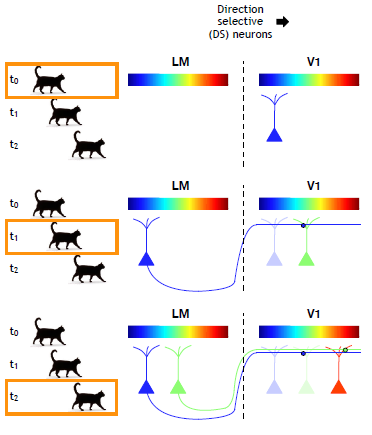
\includegraphics[scale=0.8]{2.Chapter/move.png}
\caption{Feedback signals from LM to V1 could convey predictive information about a moving object, if we consider that their wiring is biased according to their own tuning. In this example, we consider direction selectivity tuning as the criteria for the feedback wiring. \newline \textbf{Top:} A stimulus (the cat) moving in a given direction (left to right) will activate neurons in V1 with that direction selectivity and with their receptive fields located at the corresponding region where the stimulus is in the subject's visual field at that time $t_0$ (left-side, blue labeled azimuth angle). \newline \textbf{Middle:} These DS left field-of-view corresponding neurons feedforward to neurons whose RF represents the same left-side location in the visual field. These would project back into V1 neurons corresponding to positions on the middle region (green-labeled azimuth angle) activated by the stimulus at $t_1$. \newline \textbf{Down: } These neurons, activated by the stimuli presentation in that visual field region, also connect retinotopically to LM cells with the same direction selectivity. Again, these project to the neurons corresponding to the RF position ahead (right-side, red-labeled azimuth angle), activated by the stimulus at $t_2$). \newline In this way, predictions on the next cat's position, as assumed by the direction it followed at previous times, could be relayed via feedback from LM to V1 neurons.
\newline \newline \tiny{Image from the presentation by the principal co-author of \cite{Marques2018}, Tiago Marques, under the Champalimaud Internal Seminar Series on October $15^{th}$ 2017, \textit{The functional organization of cortical feedback}.}\label{cat}} 
\label{move}
\end{figure}

Different orientation selective neurons are intermingled in L1 of V1. This allows the simultaneous analysis and comparison of the effects of various tuning properties.

The experimental results showed that the retinotopic deviations depend on the feedback orientation and direction selectivities, according to simple geometrical rules - figure \ref{rules}.

Orientation-selective (OS) LM axons overspread around the retinotopically matched location in V1, and target neurons that encode positions perpendicular to the LM neurons' preferred orientation. Additionally, analysis on direction-selective (DS) axons presented that these overspread to areas with neurons encoding positions shifted from the retinotopically matched position along the angle of the LM neurons' anti-preferred direction. 

In this way, LM feedback axons could enhance visual representations in space and time, by targeting cells in V1 that code positions placed perpendicularly to the higher-level neuron's orientation selectivity or to positions placed in the opposite direction to the higher-level neuron's direction selectivity. These differ from the predictive coding hypothesis (image \ref{move}), that relied on neurons that feedback to lower-area neurons encoding positions that would be subsequent according to the stimuli direction. Instead, the work of \cite{Marques2018},  showed that feedback neurons do have organizational structure that relates to their tuning properties, but that the feedback targeting is to neurons encoding the \textit{opposite} position to that expected to be visually stimulated at following moments by the moving stimuli that drove the input neurons in the first place, when in a new position. 

\begin{figure}[H]
\center
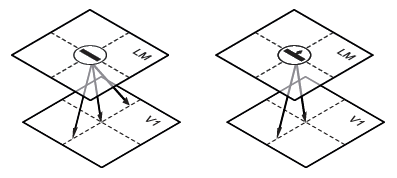
\includegraphics[scale=0.8]{2.Chapter/rules.PNG}
\caption{LM feedback to V1 functional organization according to simple geometrical rules. Planes represent retinotopic maps in V1 and LM, while bars represent preferred orientation of the LM neurons. \newline \textbf{Left:} OS inputs have biased wiring towards neurons encoding positions orthogonal to the input feedback neurons preferred orientation.
\newline \textbf{Right:} DS inputs tend to be wired to neurons that encode visual field positions along the opposite direction to the feedback input neuron's preferred motion direction.
\newline \newline \tiny{Images from \cite{Marques2018}.}}
\label{rules}
\end{figure}

This could also manifest a predictive coding strategy, but in the negative, with feedback wiring to cells that care about the non-expected positions. This could for example be explained if the wiring portraits a net inhibitory effect.

In broader terms, this study showed that there are asymmetries in the way that feedback connections are established, and that these asymmetries depend on the tuning properties of the involved cells. 
Given the possible relation of feedback and SM effects, this further motivated the scope of this project: to unravel the anisotropies and asymmetries of SM effects with moving stimuli and put them at the perspective of the possible connection circuits that could cause them.

%\cleardoublepage


\fancychapter{Technology}
\label{cap:Technology}

\textit{Developing precise and reliable tools for the spatial and temporal mapping of neuronal activity is crucial to understand the functional architecture of the brain. Radiotracer, electrophisiological, magnetic resonance, anatomic and optical imaging techniques all offer advantages and disadvantages to this end [REFERENCES]. On its part, optical imaging of neuronal activity allows the mapping of large regions of the cortex, varying in time as responses to stimuli. This can be acomplished with voltage sensitive dyes [REFERENCES], changes in the optical properties of the tissue or with the aid of genetic tools. In here, we review the utilized techniques: Intrinsic optical signal imaging that draws on the changing reflectance in the hemodynamics of the cortex and two-photon laser microscopy that takes advantage of genetic manipulation tools.}

\section{Intrinsic signal optical imaging}
\label{sec:sectiona}

\subsection{Acquiring functional maps of neuronal activity}

Neuronal activity can comprise the generation and propagation of action potentials, postsynaptic ion fluxes and potentials, neurotransmission, synaptic vesicle recycling, among other processes allocating cerebral cortex energy, along with the maintenance of glial and neuronal resting potentials. Furthermore, the cortex presents activity evoked by sensory stimuli or motor processes, but cortical populations of neurons also show spontaneous coordinated patterns of spiking activity, non-related to any sensory input or motor output.

In regards to the evoked activity, investigating the organizational and functional architecture of the sensory brain requires the means to both detect neuronal activity and to relate these responses to the external stimuli that the subject receives.  

 
% INTRODUCTION This patterns appear in slow-wave sleep, anesthesia and quiet wakefulness[REFERENCES], and the observed patterns are thought to be involved in internal processes, such as memory consolidation, mental imagery, behavioral variability or hallucinations [REFERENCES]. 

The classical approaches developed to this end study animal's brain's \textit{in vivo} by exploring electrophysiological principles: by placing electrodes inside the individual's scalp, one can extracellularly record single cells' electrical activity in a direct manner and access neuron's voltage fluctuations. Multi-unit recordings are also possible through this method. 

Other techniques include the 2-deoxy-D-glucose (2DG) autoradiographic method [SOKOLOFF ET AL, 1977] to find and measure glucose consumption in the brain. These metabolic alterations are associated to changes in functional activity and thus an acumulation of the radiolabeled 2DG, representing the integrated rate of glucose consumption, marks the activity areas of the brain.

DYES...

However, many experimental goals require extensive simultaneous recordings while these techniques require  long combersome experiments to cover large areas of the cortex. Moreover, electrophysiological mapping methods introduce considerable sampling bias in the recordings as well as poor spacial resolution ($~1 cm$), while 2-DG maps can only be analysed \textit{post-mortem}, allowing only one experimental session per animal, and can only label two stimulus at the maximum.

Imaging techniques such as functional magnetic resonance imaging (fMRI), near-infrared spectroscopy (NIRS) and intrinsic signal optical imaging (ISOI) introduce less invasive means to simultaneously access larger regions of the brain while the subject is being presented to stimuli and also enable longitudal studies by repeated imaging sessions with the same individual animal. These methods are based on variations of optically measurable properties of physiological processes associated with neuronal activity.

NIRS....

Intrinsic signal optical imaging (ISOI) enables the visualization of alterations in intrinsic optical properties of neuronal tissues, as a response to neuronal activity.

Slow reflectance light signals are intrinsicly relayed from the surface of the striate cortex due to hemodynamic responses[REFERENCES] that correlate with neuronal activity. Neuronal firing induces blood changes - neurovascular coupling - that produce a light reflectance change.

Neuronal activity requires the hydrolysis of ATP and the oxy-hemoglobin (the protein hemoglobin in red blood cells binded to oxygen) molecules in the capillaries provide the majority of the oxygen used to regenerate ATP via glucose metabolism. Thus, an active brain region is associated with a finely localized increase in oxygen demand and thus a local rise in deoxy-hemoglobin (deoxygenated hemoglobin) and a depletion in oxy-hemoglobin concentrations. This is followed by an hemodynamic response of locally increased blood flow in the capilaries and dilatation of the closeby arteries to replenish and sufice the oxygen requirements.

In this neuronally active situation, the hemodynamic response imposes a light reflectance variation, resulting from three major sources: the changes in blood volume, blood oxygenation and light scattering.

The blood volume component of the signal is the least spatially confined of the three factors, but can nevertheless yield alone functional maps, with the injection of fluorescence dyes into the bloodstream [REFERENCE].

The oxymetry signal is used for instance in fMRI techniques that identify the areas of the brain to which more oxygenated blood is being driven to, relying on how the magnetic properties of more and less oxygenated blood differ. A $1-2s$ delayed rise in oxygenation is associated to more active cells and brain usage. However, depending on the magnetic field intensity, this technique can have limited spatial resolution, as it relies on the transition phase that is also associated with the dilatation of arterioles adjoining the original activity sites which can cause signal artifacts.

On the other hand, light scattering changes (REFERENCES) allow for precise temporal and spatial functional mappings of neuronal activity. Higher neuronal activity increases light scattering due to factors like (REFERENCES COHEN 1973). This increase peaks within 2-3 s of the stimulus onset.

With these physiological events optical properties' changes, one can extract the optical signals that correlate with that variance and thus with neuronal activity. Since about $13\%$ of the energy consumption is used for maintenance of the resting state and the greater parcel of the cortical metabolized ATP costs are for action potential propagation (about $47\%$) [REFERENCES], with the remainder for processes related to synaptic transmission, the intrinsic signal has the major contribution from an oxymetry factor that relates to those inhibitory or subtreshold excitatory input processes.

\subsection{Intrinsic Signal Optical Imaging: the technique}

In the technique used in this work, ISOI, the signal brings about information on the oxy-hemoglobin concentrations during neuronal activity. For both anesthetized and awake animals, the typical ISOI signal follows a tri-phasic structure: An initial dip, a negative peak at about 4-6s after stimulus onset, and a large rebound [GET REFERENCES].[GET IMAGE] 

Illumination by a stable output source at the red wavelenght level of $540 nm$ optimally excites the oxygenated blood flow, while the de-oxygenated blood reflects less light at this wavelength [REFERENCES]. 

These differentiated properties enable the mapping of the most active, de-oxygenated brain areas at the time of the initial local deoxy-hemoglobin increase, since these regions will reflect less red light than the inactive, amply oxygenated cerebral areas.

ISOI utilizes this principle in brain areas which can be reached by light (around $500 \mu m$ maximum). In an animal with a window implantation and illumination of its primary cortex surface, one can record the brain area with a charge-coupled device (CCD) camera to monitor the changes in the reflected light signal from each region of the primary cortex of the subject while this animal is presented to stimuli. In this way, one obtains maps that make correspond the stimulation that the subject receives - visual, somatosensory, auditory [REFERENCES]- to the observed refleted light signal profile at that time interval and in that brain region, whitin some relatively high temporal ($80 ms$) and spatial resolutions (in the order of $100 \mu m$) [REFERENCES].

The properties of this signal in amplitude and temporal dynamics, as well as of their components, depend on both the stimuli and on the wavelength of the ilumination light that the brain is receiving[REFERENCES].


The signals' information is extracted by calculating differences between unstimulated baselines and post stimulation time points. For each stimulus, multiple repeatitions are held and the respective signals averaged across the same time points.


Furthermore, in regards to the stimuli dependence of the signal's timecourse, the ISOI signal can be divided into a global stimulus-non-specific response and a local stimulus-specific response that is observed from functionally organized cortical columns[REFERENCE]. This latter component stands as the actual mapping signal. 

[REFERENCE] found that the signal's rise time and time to peak were nearly identical for both short and long stimulus durations. However, the  relaxation time course of the signal does depend on the stimuli duration, which imposes an appropriate inter-stimulus interval and/or aware analysis.
\section{Calcium indicators and transgenic lines}
\label{sec:sectionb}
\section{Two-photon laser scanning microscopy}
\label{sec:sectionc}

Neuronal phenomena can be relevant in broad scale ranges, both spatially and temporally. With high resolution, sensitivity, contrast and being able to track events over large cortical ranges, two-photon excitation (2PE) laser scanning microscopy provides a way of accessing fluorescent objects, such as the GCaMP6 expressing neurons, by selectively exciting them and detecting the produced light signal. This technique can furthermore be applied to living or intact tissue, with minimal photodamage (phototoxicity and photobleaching). The probability of detecting a signal photon per excitation event is greater than with previous techniques, especially for imaging deep in scattering tissue.

Two low-energy photons (deep red and near IR) are sent by a focused laser to a fluorophore unit and excite, in combination, the higher-energy electronic transition required for the emission of fluorescent light. 2PE is a nonlinear process, as the absorption rate depends on the squared value of light intensity. This intensity drops quadratically with the distance from the focus. Therefore, if the numerical aperture objective is small enough, this excitation is localized, and the excitation can affect a very small focal volume and produce good 3D contrast and resolution.

Another advantage of 2PE is in its relation with scattering. As photons enter tissue, they scatter and deviate their paths according to inhomogeneities found in the refractive index of the medium, and this reduces the amount of light delivered to the focus and from the fluorescent molecule to the detection apparatus. However, 2PE uses near IR beams that penetrate tissue better than visible waves (as used in one-photon microscopy); the non-linearity of 2PE also contributes to the reduced scattered photons; and finally, since the excitation is localized, all the fluorescence photons coming from the excited molecule, even if scattered, portray useful signal, not being lost and not contributing to background noise.

Typically, a laser is focused on a given target plane and scanned over the sample. When an excitation occurs, it is detected by photodetectors. These responses are then summed over some microseconds and mapped to single pixels of an image.

The lasers used for this method should be powerful enough to compensate for the small two-photon cross-sections and produce sufficient signal levels. Moreover, 2PE efficiency increases as the inverse of pulse duration, and the device should thus be suitable for short light pulses. Mode-locked Ytterbium-doped and Cr:forsterite lasers suffice these requirements for the considered wavelengths.

Objectives are used for the essential focusing of the laser beams. Another important consideration regards the detectors: These should cover large sensitive areas (millimeters), as well as contemplate good gain, quantum efficiency, and other important thresholds. Photomultiplier tubes (PMTs) are usually applied for this purpose.

\cleardoublepage

% %%%%%%%%%%%%%%%%%%%%%%%%%%%%%%%%%%%%%%%%%%%%%%%%%%%%%%%%%%%%%%%%%%%%%%
% Dummy Chapter:
% %%%%%%%%%%%%%%%%%%%%%%%%%%%%%%%%%%%%%%%%%%%%%%%%%%%%%%%%%%%%%%%%%%%%%%

% %%%%%%%%%%%%%%%%%%%%%%%%%%%%%%%%%%%%%%%%%%%%%%%%%%%%%%%%%%%%%%%%%%%%%%
% The Introduction:
% %%%%%%%%%%%%%%%%%%%%%%%%%%%%%%%%%%%%%%%%%%%%%%%%%%%%%%%%%%%%%%%%%%%%%%
\fancychapter{Technical Implementations}
\label{cap:chapter}

\textit{As the first part of this thesis' work development, hardware adaptations were implemented and software protocols were programmed for the real-time behavioural control and stimulus presentation to be used in the experiments. This was done with the open-source arduino-based system Bpod, by adapting the previously used microkernel-based system Bcontrol. This required the development of a synchronized graphical user interface, the communication between a governing machine, a microscopy apparatus, a stimuli monitor and a bpod device, within minimal processing time, as well as different states matrices and protocols for each type of visual stimulation display - RF mapping, tuning mapping and SM properties investigation.
Moreover, the system also required proper functionality within the software controlling the two-photon microscope, which was enabled by the trigger and configuration settings of the software ScanImage.}

\section{System's scheme}
\label{sec:sectiona}

The experimental procedure of visual stimuli display involved four main components in communication of parameters, configurations and triggered synchronization: A governing machine and a stimulus display matlab instances, a Bpod device and the set of two-photon laser microscopy appliances and software. 

\begin{figure}[H]
	\centering
		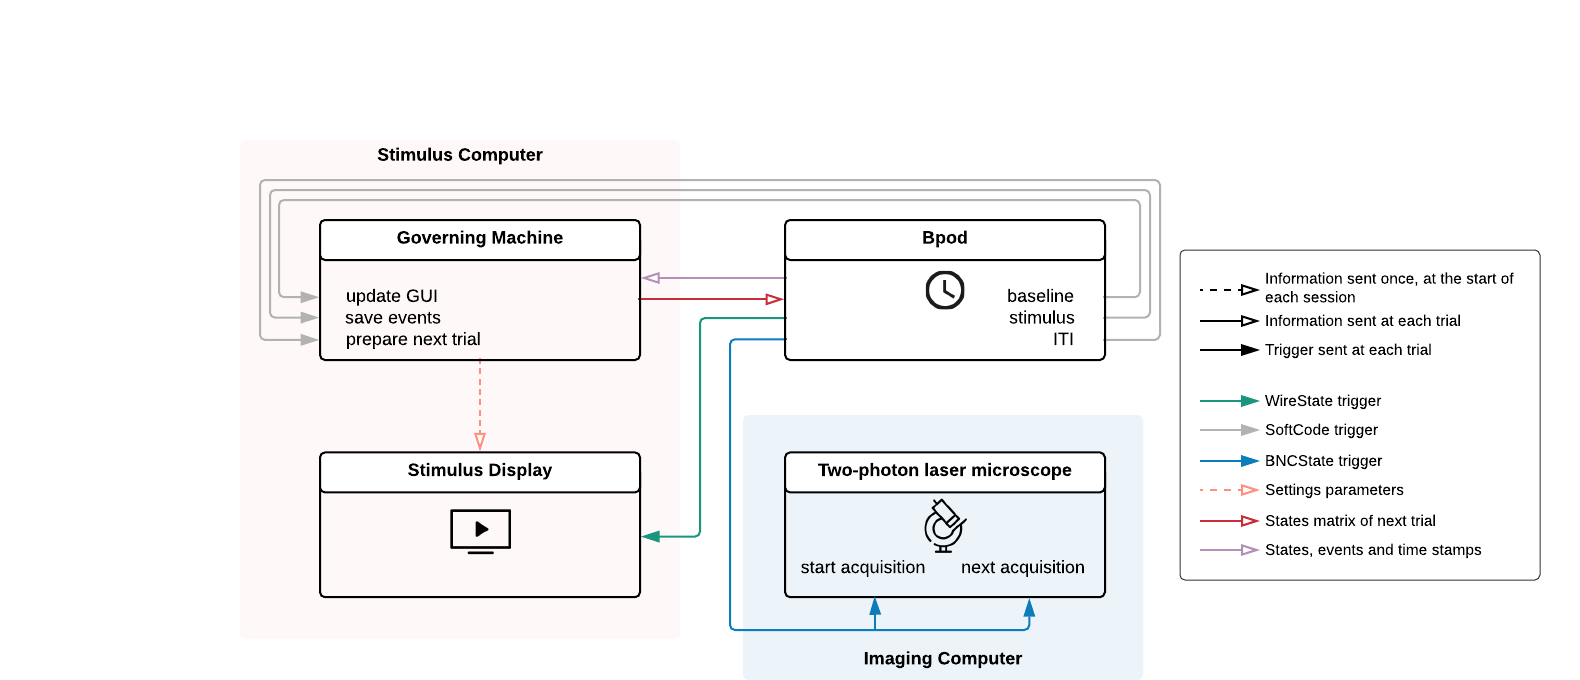
\includegraphics[width=1\linewidth]{3.Chapter/systemtechnical.png}
	\caption[c1]{Setup and connections scheme of devices used for stimuli presentation and real-time imaging.}
	\label{fig:systemtechnical}
\end{figure}

The governing machine and the stimulus display were controlled by one of the computers, called here stimulus computer.

The governing machine held the Graphical User Interface (GUI) as well as all of the computations and running protocols with Bpod's software for saving the stimuli settings and preparing the stimuli configurations and states matrices for the different trials. 

The stimulus was displayed in a second monitor connected to this stimulus computer and operated within a second matlab instance of routines coded with Psychtoolbox software for interfacing between Matlab and the computer screen. This Matlab instance loaded, at the beginning of the session, all of the stimuli settings that were saved in the bpod's Matlab instance. With a counter, the script iterated the full trials structure, displaying the applicable stimuli at the proper times. This timing synchronization was enabled by triggers received in a NI-DAQ data acquisition board. 

The bpod apparatus produced these triggers, connected to the system and taking advantage of a precise internal clock. Having received each trial's state-matrix specifications from the governing machine with enough buffer time, bpod produced the appropriately timed states - the main ones being the baseline, the stimulus and the ITI - and sent the required triggers at each stage. At each trial, in the beginning of the baseline period, a trigger was sent to the governing machine to update the GUI to show the current trial stimuli specifications; during the stimulus presentation, another trigger was sent to save the events of the previous trial and during the ITI an instruction was sent for the governing machine to prepare the next trial by computing the next states matrix with the new trial's stimuli configurations. Bpod also sent, at the beginning of the stimulus display state, the trigger for the stimulus computer second matlab instance to display the loaded and prepared stimulus in the screen visualized by the animal. Finally, at the beginning of the baseline and in the end of the ITI of the proper trials, a trigger was sent to the called imaging computer that held the software controlling the two-photon laser microscope for respectively starting and afterwards completing and proceeding to the next scanning acquisition. 

The two-photon laser microscope had different components: The laser apparatus with the mirrors, lenses, beam-splitter and remaining light path enforcers; the objective enabling both a bright field and a two-photon configurations; the synchronization device, a NI-DAQ data acquisition board for receiving Bpod's triggers, and finally the imaging computer that operated the controlling software application ScanImage 4 for laser scanning microscopy. This was also the computer that saved the raw image sets acquired from the two-photon scannings at each protocol session.

The information sent and triggers used the different physical wiring possibilities: Firstly, \textit{SoftCodes} were sent from bpod to the governing machine's computer. These are code that go via the USB port that connected these devices. From bpod to the stimulus display NI-DAQ board, \textit{WireStates} were used, from wire ports in bpod, and, to the two-photon NI-DAQ board, \textit{BNCState} triggers were sent, from bpod's BNC ports. On the other hand, the information about states, events and trial time stamps was sent at each trial via USB from the Bpod device to the bpod's governing machine matlab instance and then saved with its own software. 
From the governing machine, information was sent as the following trial's state matrix, to the bpod device also via USB (Softcode) and the next trial's settings were sent to the stimulus display matlab instance by saving them at the beggining of  each protocol session in a file that was then loaded in the stimulus display matlab before starting the session.
\section{Bpod}
\label{sec:sectionb}
\subsection{Motivation and previous system}
\label{subsec:subasectionB}

Bpod encompasses a flexible open-source platform for developing stimuli presentation, behavioural protocol and reinforcement experiments. The system builds on a parallel processing model, software functions are written in Matlab/Python and the firmware builds on Arduino language. The system was develloped in Kepecs Lab [REFERENCES] at Cold Spring Harbor Laboratory and is currently maintained by Sanworks LLC, a company focused on open source neuroscience tools.

The main capability of the system is its precise time measuring feature. In imaging and even more so in electrophysiology animal experiments, it is paramount to control and synchronize the timings of stimuli presentation, behaviour/neuronal activity detection and states sequencing in the different setup compontents. Precise triggers from a governing machine to a brain activity measurement device - the two-photon setup, in this case -, to a stimuli display - visual or not - or behavioural gadgets allows reliable functional brain mappings, and appropriate analysis and interpretation of an animal's brain or physical responses.


Prior to this implementation, the Cortical Circuits Lab was using B-control for mice's behavior measurement and finite states machine, a system developed by Brody Lab at Princeton University [REFERENCES]. In fact, Bpod builds on B-control's parallel processing design idea: the state machines for each trial are constructed in Matlab in a governing machine and executed in a separate device. For B-control, this is a separate microkernel real-time Linux computer. Bpod, on the other hand, uses an Arduino microcontroller network with finite state machine firmware for the real-time processing. This provides higher level software tools for adapting and constructing protocols, as well as a simpler, less expensive hardware solution.


Bpod entails two items: The device that provides the state machine substract, with a precise internal clock, output ports for TTL triggering, input ports, behavior ports with infrared photogates, LEDs and solenoid valves for dispensing liquids; and the software that, run in the governing machine, provides functions with which to code the states matrix, to equip the system with a GUI and the necessary supporting functions for each protocol and to implement functioning communication between the Bpod device and the other components - in  the case, the stimuli computer and the two-photon computer. 

The Bpod system presents the following five principal functionalities:

\begin{itemize}
\item Ensures the precise triggering between the Bpod device and the involved components - microscope set, stimuli screen and governing machine;
\item By enabling the implementation of a GUI interface, this equips the user with a practical way of setting the characteristics of the stimuli at the start of the experimental session;
\item The GUI also facilitates the monitoring of the stimuli presentation sequence at the same time as it is happening in a given session: the current trial with its correspondent stimuli properties is shown, as well as the appropriately timed states - baseline, stimuli presentation, ITI and auxiliary states - within the running protocol. Moreover, the states machine can be started - with the last submitted stimuli settings -, stopped, paused, continued or restarted by the user at any time, keeping the synchronization and . [GET IMAGE] 
\item Automatizes the saving of the data structures containing a session's stimuli sequences, as well as the time stamps related to the state matrix that was run, with the computer times for the start of each state or event leading to a state change.
\item Although not used during this work, as the experiments only regarded stimuli presentation, and because the animals were kept anaesthetized, minimizing the need for further controls, one of Bpod's main functionalities regards the measuring of the animal's behaviour. The state machine receives these discrete behavioral events and can rapidly respond by changing the animal's environment. For instance, by connecting Bpod to treadmills, one can measure a small animal running behaviour;  by connecting Bpod's appropriate ports to water valves connecting to drinking tubes, those can be controlled for implementing a reward system during reinforcement experiments; Bpod also detects the instant when discrete events happen. This can be used for example in decision making experiments: a snout entering a port or a tongue blocking a photogate can indicate an animal choices. High quality audio stimuli can also be produced with the integration of Psychtoolbox. These features deem the Bpod system a practical tool for various behavioral paradigms: two alternative forced choice (2AFC), go/no-go decisions, reaction time measurement, self-stimulation (repetition of physical movements), social value measurement, among other possibilities. 
\end{itemize}

The access to these functionalities is to be understood as provided that the user develops the programming protocols and optimizes it to meet the requirements that the experiment entails. Bpod system is not a ready to use package: it requires an understanding of the functions provided, Matlab or Phyton coding, and all of the hardware communication specifications in each protocol's case. More fundamentally, the user should have a clear planning of the specific communication scheme to use in their case, as well as of the GUI and states machine development and the important variable structures with the information to be produced, exchanged between components and saved. Documentation is available in [BPOD WIKI] and technical support can be found in the cooperative [BPOD FORUNS].

The development process started in a 45-days internship at the Cortical Circuits Lab in 2016, in which l adapted a stimuli presentation protocol from Bcontrol to Bpod, by familiarizing with both Bpod and B-control syntaxes and function environments. This work was carried with the mentorship of Leopoldo Petreanu and the guidance of Tiago Marques through the B-control environment protocol that he had developed and that the Laboratory had been using. The protocol enabled full-screen moving gratings or random dots, under different stimuli properties - timings, screen stimuli positioning, number of repetitions, luminosity values, gratings versus random dot stimuli type probability, orientation, direction, dots speed, density, coherence and size, gratings temporal and spatial frequency - in pseudo-randomized selections according to a general user's requirements with the possibility for fixating a seed, facilitating troubleshooting. At the time, this protocol was tested with the same stimuli Psychtoolbox code written for B-control. Since then it was further used in electrophysiology experiments in the Laboratory by the PhD student Gabriela Fiorze.

In this thesis' protocols development, I used  this previously coded and tested protocol as a basis. However, in this case, besides having to adapt the states machine, GUI, main and support functions from the governing machine, it was also necessary to develop new stimuli protocols with Psychtoolbox [REFERENCES] and to understand the triggers, ScanImage software [REFERENCES] and hardware connections made with the two-photon computer setup. Furthermore, at the time I used a Bpod State Machine device at version 0.5 that was switched at this point for version 0.9, with slight differences in hardware, as well as in the software functions and firmware.

In the following chapters I will go through the three protocols I developed for this thesis' experiments. For these, as in the originally developed Bpod protocol, I focused on the protocols user-friendliness, minimal processing time and in the flexibility of the code for both other similar experiments and for adaptations to other paradigms.

\subsection{Bpod Hardware implementation, specifications and alterations}
\label{subsec:subbsectionB}

The Bpod State Machine device runs on a Arduino Due 32-bit processor with 84MHz clock speed. The bill of materials can be found at the device's wiki [REFERENCES]. 


\begin{figure}[H] \centering 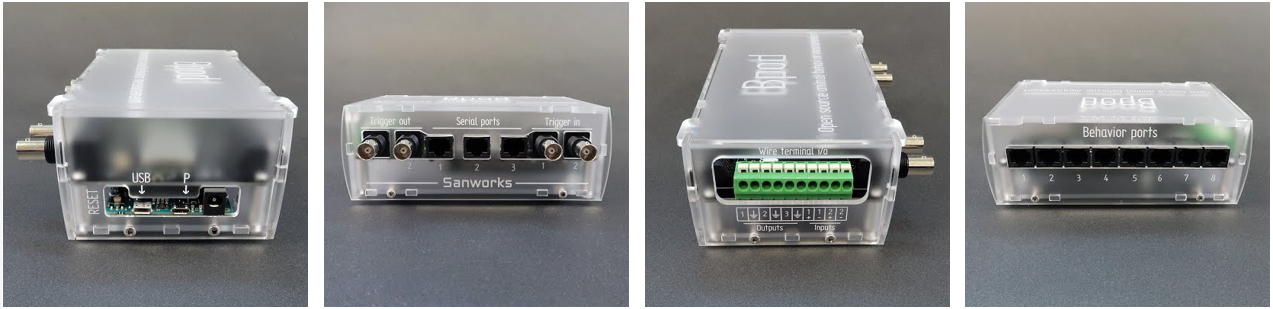
\includegraphics[width=16cm,height=16cm,keepaspectratio]{Figures/3.Chapter/bpodangles.png} 
\caption{Perspectives of Bpod State Machine device version 0.5, identical parts as in version 0.9, but with fully transparent box container design. Images from Sanworks Bpod wiki page [REFERENCES].} 
\end{figure}


Firstly, the device contains a 'reset' button to reset the device if necessary and two USB port jacks - an Arduino's native USB port to connect to the governing machine and a programming port for cases when it is necessary to re-upload Bpod's firmware. Moreover, there also is a power barrel jack for cases when the USB port is not supplying enough power to the device - this power jack was used in troubleshooting but, with the final setup, the power from the USB proved to be enough.


In Bpod, there are four BNC channels, two input and two output. The output channels are constructed to serve as 5V triggers, as Bpod can produce events and send triggers with TTL logic through them. These were initially used here to connect to the two-photon computer's NIDaQ board, one of them as a 'start acquisition' trigger and the other as a 'next acquisition' trigger. 

Bpod also has bare wire terminals, with TTL logic. The spring terminal channels are of two inputs (2.5V to 5V) and three outputs, all with the respective grounds. The outputs here are 3.3V TTL pulses. In this thesis work, I required one extra trigger port to be connected to a NiDAQ [THE WHITE THING]. This WHITE THING was by its turn controlling the stimuli screen. One of these wire channels was thus used to portray trigger pulses. For this, to be assured that there was sufficient voltage at this port (5V, according to the WHITE THING specifications [REFERENCE]), the Bpod circuit was altered in the Champalimaud Foudation IT platform with a 3.3V to 5V voltage amplifier at this wire output channel [HOW? CHECK].

Although not used in these experiments, the apparatus additionaly contains behavior study components: An ethernet that can connect to a lickometer or a nose port, as well as 8 behavior ports, each with an LED with software-adjustable intensity, a solenoid valve (12V, 150mA), and an infrared photogate. Also not necessary for these experiments, the device also contains serial ports that allow to connect it to other Arduino boards or modules that can be acquired from the same company.




\section{Software: Governing machine protocols and stimulus presentation}
\label{sec:sectionc}

Bpod's software allows to load user-made protocols and run them within the built-in bpod interface, joined with the protocols' specific GUI windows.

In this project, three protocols were developed for different ends: receptive field mapping, tuning measuring and studying the spatial structure of surround modulation.

Each of these were subsequently used in mice experiments. The produced data was also analysed, validating the method and tool in the three protocols. 

The RF protocol served to find the RF positions after each experimental session and assess if the majority of the measured cells' RFs was centred at the corresponding display monitor center, as desired. Specifically, the obtained RF maps either indicated, in combination with the retinotopy maps, in which directions one should move the objective to correct the imaging position in following sessions or confirmed that the objective and mouse placing was appropriate. Furthermore, this data was also combined with the SM protocol's results for RF position-dependent analysis of the SM effect.

The tuning protocol was implemented to measure the selectivity of cells in a flexible array of conditions. The data collected from this protocol was analysed and some cell's tuning examples are shown in \ref{cap:Results}. This analysis served to validate the protocol and aided in troubleshooting the SM analysis. Moreover, this protocol was also used to find the RF centred imaging positions during experiments. 

Finally, the SM study was the main focus of this project's experimental component, and the obtained results are presented in \ref{cap:Results}. The implementation of this protocol allows the presentation of any configuration with center and surround moving gratings' patches, in any combination of the four cardinal plus center positions. For this project's purposes, 124 were chosen, in a given set of grating frequencies and stimuli sizes.

Each of these protocols follows a similar structure of five files, each with different case functions:

\begin{itemize}
\item \textbf{main}: initiate, submit, start, prepare next trial, synchronize GUI, save settings and events, process trial completed, restart and stop;
\item \textbf{states matrix}: prepare matrix, run;
\item \textbf{GUI}: initialize, synchronize;
\item \textbf{SoftCode handler instructions}: maps SoftCode bits to be sent in the states matrix to functions: main(prepare next trial), main(save settings events) and main(synchronize GUI);
\item \textbf{Support functions}: set session, set next stimulus and save parameters.
\end{itemize}

In bpod's built-in interface, one can set the mouse ID, load the settings to use as default and then call the desired protocol. 

At this point, the main file is called to initiate the protocol: This by its turn calls the GUI initiation function, which initializes the settings variables in a global structure S, in different fields according to the required type of GUI to be used (an edit box, a toggle button, a slider, an edit array, an array display or a push button). This organization allows to then easily initialize handles of each parameter's user interface control, depending on the type of GUI.

In the ScanImage interface at the imaging computer, the appropriate configurations must be set by the user before starting the stimuli and bpod protocol - The user must choose the number and positions of the imaging planes, imaging trigger ports, brightness of the brain recordings displayed, as well as the path and name for the recorded movies. Then, the imaging system can be instructed to await the external triggers that will come from bpod.

In bpod's computer, once the user chooses the intended parameter values in the GUI and clicks the \textit{submit} button, the GUI is synchronized, the current trial variable is set to 1 and three support functions are run on S: 

First, the session is set: An angular coordinate system is computed, converting monitor $(y,z)$ coordinates in azimuth and elevation, from the perspective of the mouse:

\begin{equation}
elevation(º)= - \left[ \dfrac{\pi}{2} - \arccos \left( \dfrac{z+z_0}{\sqrt{d^2 + (y + y_0)^2 + (z+z_0)^2}} \right) \right] \dfrac{180}{\pi}
\end{equation}

\begin{equation}
azimuth(º)= \dfrac{\arctan(y-y_0)}{d}\dfrac{180}{\pi}
\end{equation}

with $y_0$ and $z_0$ the positions in respectively the horizontal and vertical monitor axis centred perpendicularly to the mouse's gaze and $d$ the distance from the mouse's eye to the center monitor position.

In the RF case, grid positions can be produced from the settings and randomly permuted in a presentation sequence, along with a key for the respective gratings direction sequence also in pseudo-randomized order.

Similarly, for the Tuning protocol, all of the possible combinations of center azimuth, center elevation, stimulus size, temporal frequency, spatial frequency and moving gratings direction are randomly permuted, within the total number of trials, with the specified number of repetitions for each trial type. This maps a pseudo-randomized sequence for every dimension of stimuli properties that is saved and displayed in a GUI variable.

Finally, for the SM protocol, every trial type is also repeated a specified number of times, put into an array that is then shuffled and creates a complete order of stimuli presentation. Each value in this final array corresponds to values in other variables that are also saved and displayed: these represent if the center, left, right, top and/or bottom patches are being presented, and if so what are its gratings directions.

The second support function sets the next stimulus, by updating the current stimulus variables to the first trial case, according to the order in the total stimuli properties arrays created (position and direction sequence for the RF protocol, for example).

Then, in the third support function, the relevant parameters for the stimuli graphical presentation are saved in an external \textit{next stimulus} file, to be read and loaded in the psychtoolbox stimuli display Matlab instance.

The GUIs are synchronized to the newly computed values of the parameters, and the first states matrix' preparation is called.

The matrix sent to the bpod device follows the flowchart in figure \ref{fig:bpodimplementation}.

\begin{figure}[H]
	\centering
		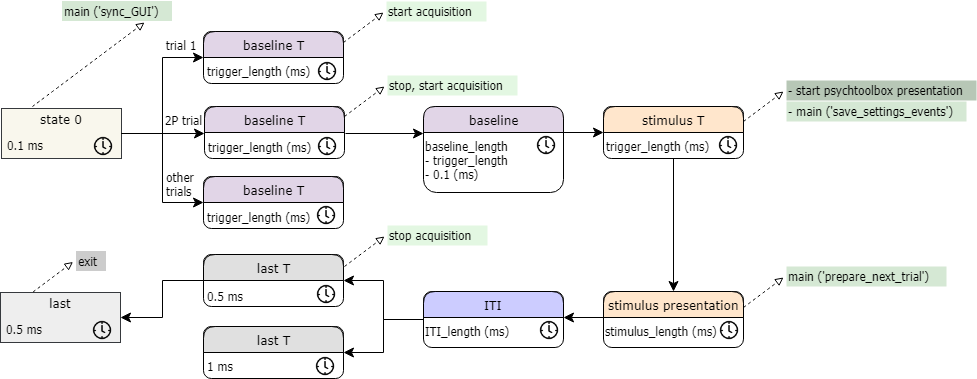
\includegraphics[width=1\linewidth]{3.Chapter/bpodimplementation.png}
	\caption[c1]{Flowchart of the states matrix implemented for the three developed protocols (RF, Tuning and SM). Each state is represented by a name, a timer, state change conditions and output actions. The states machine is formed by three principal states: a baseline, a stimulus display and an ITI. Trigger ("T") states were added, with \textit{trigger length} times corresponding to the duration of the according pulse. All of the state changes were to happen at the end of the internal timer at the current state. The output actions are represented by dashed arrow lines: these represent triggers to the imaging computer (lighter green) through BNC connections, to the NIDAQ of the psychtoolbox matlab instance (darker green) through a wire connection and internal triggers to other functions in the governing machine, through USB connected softcodes (medium green).}
	\label{fig:bpodimplementation}
\end{figure}

After this \textit{submit} process, the user can initiate the psychtoolbox script written for the given protocol at use, in a second matlab instance. This script opens the NIDAQ device and configures it to receive triggers, then opens the screen in the setup monitor in front of the mouse, and loads the session settings in the \textit{next stimulus} file. 

In the case of the RF protocol, this computes a checkerboard mask and divides it into a mask for each grid cell's position figure. It also prepares full screen moving gratings at the settings' frequencies and contrast levels, going in the indicated sequenced directions, within a set of frames in the required number for completing the time length of the stimulus presentation, acording to the monitor's frame rate. Finally, these are combined into textures - sequences of images - that correspond to each trial type and that are saved in a structure for that trial type and every frame of that trial.

The preparation of display movies for the Tuning protocol is done in a similar way: Masks are produced for a circular patch with the possibly multiple sizes and centre positions indicated in the stimulus file, and full screen moving gratings are computed in the brightness levels specified, and for the spatial and temporal frequencies at hand, which can also be more than one in the same session. Then the gratings are masked, forming sets of images (textures), each corresponding to a type of trial and saved in a structure.

For the SM protocol, five masks are produced with the sizes and positions indicated, one circular patch for the center stimuli, and four cardinal quarter-torus for the surround patches. Gratings are drawn at the instructed frequencies and contrasts, also in full-screen. This means that the final textures, maskings of the moving gratings, form in-phase center and surround patches with the same grating properties. These textures regard combinations of the center and surround patches, and each is saved in correspondence to one trial type.

When a trigger reaches the entrance specified in the NIDAQ device, the corresponding trial texture frames are drawn in sequence and the timing between the previous trigger and the current one is displayed on the matlab command window for monitoring possible skipped triggers.

When the textures are loaded, the user can click the start button, which first saves the submitted settings in a stimulus file and then calls the states matrix to run.

Softcodes sent from the bpod device to the governing machine allow processing of given instructions, while the states matrix is simultaneously being run, thus enabling parallel actions. 

As represented in image \ref{fig:bpodimplementation}, in the beginning of a trial, a trigger from the bpod device to the governing machine dictates the GUI's synchronization, updating the displays to the current trial properties. Another softcode is sent, before the stimulus presentation, to save the events and time stamps from the previous trial in a file in the governing machine, in the case of trials after the first. Finally, a \textit{prepare next trial} instruction is sent in the middle of each trial. In parallel to the stimulus presentation, this instruction internally increments the current trial variable, then runs the \textit{set next stimulus} support function and calls the \textit{prepare next matrix} function. This ensures that the next trial variables, GUI and matrix are ready when the current trial finishes and the next \textit{run states matrix} instruction is sent.

During the trials, triggers are sent to the imaging computer to acquire  sequenced images of the animal's brain. The user can decide how many trials are added in every recorded set of images, by changing a GUI variable. Thus, at the beginning of the first trial, a \textit{start acquisition} trigger is sent to the two-photon system and then, at the beginning of every first trial of the imaging sequence, a\textit{next acquisition} trigger is sent, to stop the recording of the images in the previous set and a \textit{start acquisition} follows to record the next images in a new set. A displayed variable in bpod is incremented every time these first trials are reached. In combination with a scanImage interface's display of the number of acquisitions held, the user can monitor the synchronization between bpod and the imaging system.

Once the current trial reaches the last state and the current matrix is finished, the main's \textit{trial completed} function is called. This increments the current trial variable and calls the run states matrix function again. The system enters the prepared states matrix, with the variables, GUI and matrix timings and conditions correspondent to the incremented trial.

The recurrent cycle continues until the last trial is completed, in which case the run states matrix instruction is not sent again, the events and trial stamps from this last trial are saved, and the bpod protocol stops. 

At this point the psychtoolbox script will also finish and the timings displayed in respect to the intervals between triggers can also be saved.

In addition, the bpod protocol can be paused, restarted or stopped at any point. The pause instruction is handled at the beginning of a new trial and, when restarted or stopped, the settings, events and time stamps from the interrupted session are saved, to still retain this information for possible analysis.

In summary, a session runs through sequenced trial matrices. Each of these is created in advance, simultaneously to the running of the preceding matrix. At each trial and state, bpod sends the appropriate triggers to the two photon system for image acquisition, and to the NIDAQ device, for stimulus presentation. In addition, bpod also sends triggers to the governing machine for parallel processing: updating the GUI displays, saving information and preparing the next matrix. Image \ref{fig:examplediagram} shows a simplified diagram of an example mini-session of 4 trials with the two-photon image acquisitions being started at every 2 trials.

\begin{figure}[H]
	\centering
		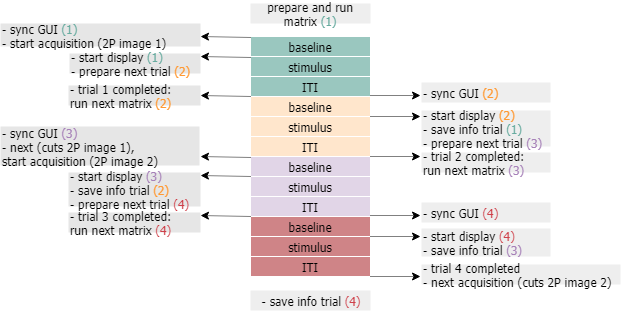
\includegraphics[width=0.8\linewidth]{3.Chapter/examplediagram.png}
	\caption[c1]{Diagram of the simplified states sequence in a session of 4 trials and two-photon acquisition triggers sent every two trials. The gray boxes indicate instructions, and the arrows represent the different trigger instructions sent at the state in its trailing edge. The colored parentesis refer to the trial that each instruction relates to. \label{fig:examplediagram}}
	
\end{figure}
%\section{Hardware: Trigger wiring and two-photon microscopy}
\label{sec:sectione}

\subsection{Triggering}
\label{subsec:subasectionD}

\subsection{Two-photon laser microscopy}
\label{subsec:subbsectionD}
%\section{Hardware: Trigger wiring and two-photon microscopy}
\label{sec:sectione}

\subsection{Triggering}
\label{subsec:subasectionE}

\subsection{Two-photon laser microscopy}
\label{subsec:subbsectionE}
%\section{Instrumentation}
\label{sec:sectionf}
\cleardoublepage

\fancychapter{Experimental Methods}
\label{cap:Experimental-methods}

\textit{Over the experimental process, the appropriate settings of both the animals' state of alertness and of the visual stimulation were chosen as an operative practical balance. In this chapter we describe the methods and specifications of the animals' care and craniotomy cirurgies, as well as the settings of the ISOI and visual stimulation sessions.}

\section{Animals}
\label{sec:Animals}

All procedures were approved by the Champalimaud Centre for the Unknown Ethics Committee and carried under the stipulations of the Portuguese Direção Geral de Veterinária. Mice were held in individual cages on a reversed light-dark cycle with access to food and water. Mice were exclusively used for the experiments regarding this thesis' work.

Cells' somata in V1 layer 2/3 of four Thy1-GCaMP6s ?? male?? mice (?? Laboratory stock no:??) were imaged.

Prior to the imaging experiments, once adults (?? to ?? weaks old), the mice underwent chronic window implantation surgeries. A circular craniotomy of diameter $4mm$ was performed over each mouse's left visual cortex, leaving the dura intact. The imaging windows were constructed using two layers of microscope cover glass (Fisher Scientific, no. 1 and no. 2) and UV-curable optical glue. A window was placed into the craniotomy using black dental cement and an iron headpost was attached to the skull with dental acrylic. The subjects were kept under isoflurane anesthesia, as well as Bupivacaine ($0.05\%$; injected under the scalp) and Dolorex ($1 mg/kg$; injected subcutaneously), serving respectively as local and general analgesia. Eye moisturing was insured with ophtalmic ointment (Clorocil, Laboratorio Edol).

For both the ISOI and visual stimuli protocols, the animals were lightly anesthetized with isoflurane ($1\%$) and injected intramuscularly with chlorprothixene (1mg/kg), a muscular paralyzer to circumvert the need for higher anesthesia concentrations which could depress the recorded neuronal responses. Mice were headfixed by the headposts during all of the visual stimuli presentations and their eyes were protected and kept moist with silicone oil (Sigma-Aldrich) in thin, uniformly coated layers.

\section{Visual stimulation}
\label{sec:Visual-stimulation}

For both the ISOI and visual stimuli protocols, an LED display (BenQ XL2411Z, 144-Hz monitor, stimulus presented at $60 Hz$) was used. The screen was placed at $15 cm$ from the mouse's right eye and  aligned at $30º$ to the axis of its nose-line. The stimuli were produced and presented using Matlab and the Psychophysics Toolbox (see \ref{cap:TechnicalImplementations}. 

\section{Intrinsic signal optical imaging settings}
\label{sec:Intrinsic-signal-optical-imaging-settings}

The course of action with each craniotomized mouse started with the performance of intrinsic signal optical imaging (ISOI) over the mice's primary visual cortex and surrounding visual areas to obtain a reasonable spatial resolution retinotopic mapping of the temporaly dependent hemodynamics of the accessed brain while moving visual stimuli was presented to the animal on a monitor aligned to the center of the mouse's right eye and forming a $30º$ angle with the animal's nose-line.

The stimuli consisted of a checkerboard of alternate flickering light/dark squares ($5 Hz$) that was masked to continuously expose only a periodic drifting stripe of the grid in four consecutive cardinal directions ($12 s$ period, $20º$ width, 80 times for each direction) - an horizontal stripe going from the top to the bottom of the screen, vice-versa, a vertical stripe going from its left to its right or in the opposite direction.

The cortical surface of an head-fixed mouse was illuminated with a $620 nm$ red LED to allow the intrinsic hemodynamic signals to be recorded as optical images of reflectance change correspondent to cortical activity. This recording was held using a Retiga QIClick camera (QImaging) controlled with Ephus with a high magnification zoom lens (Thorlabs) at $5 Hz$ focused under the cranial window, at the brain surface. A $535 nm$ green LED was also used to obtain an image of the cortical vasculature.

For each animal, this resulted in a retinotopical map of $512 \times 512$ pixels, representing $400 \times 400$ of cortical area. This corresponded to the color-map of cortical encoding of both azimuth and elevation stimuli locations, superimposed on the image of the mouse's vasculature (images \ref{vessels} and \ref{mapping}). These correspondence figures were subsequently used as a first-approach guide to encountering the V1 positions aimed for imaging - those whose neurons responded to stimuli in the center of the mouse's visual field where the central stimuli were displayed during the following two-photon microscopy imaging sessions.
\begin{figure}[H] \centering 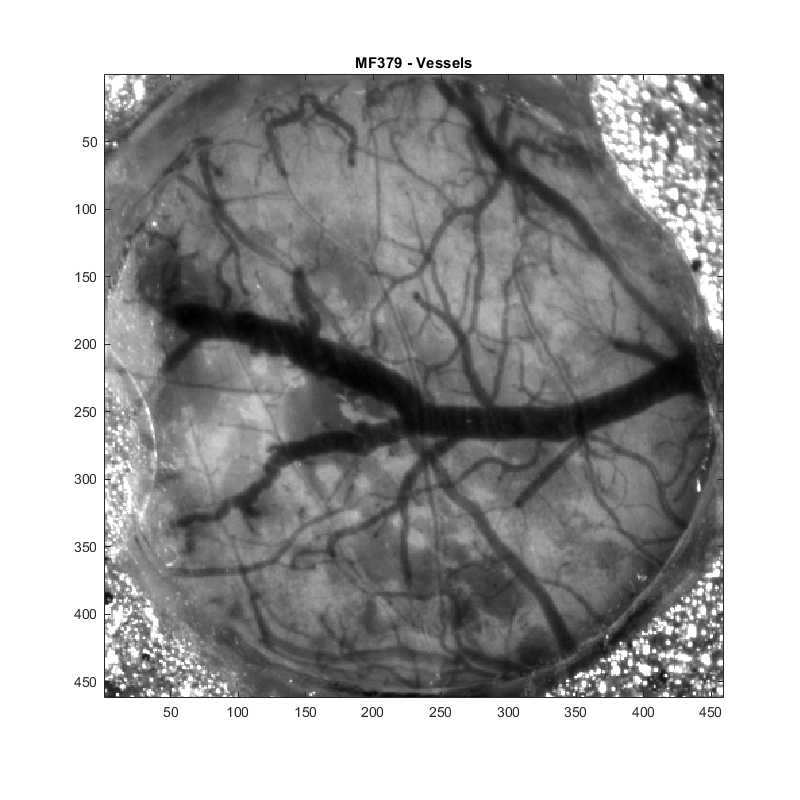
\includegraphics[width=7cm,height=7cm,keepaspectratio]{Figures/7.Results/intrinsic/MF379_Vessels.png} 
\caption{Vessels image obtained with ISOI for an example animal.}
\label{vessels}
\end{figure}
\begin{figure}[H] \centering 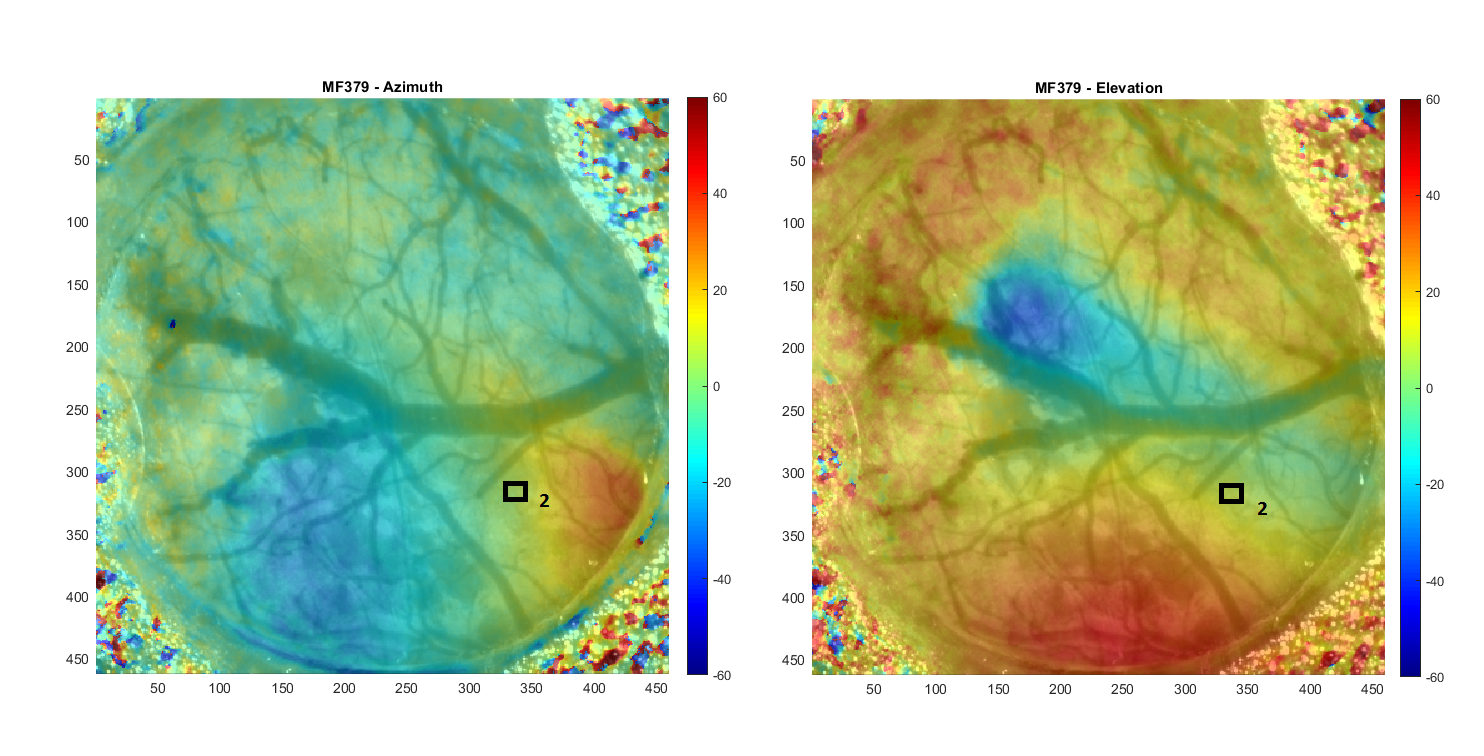
\includegraphics[width=13cm,height=13cm,keepaspectratio]{Figures/7.Results/intrinsic/mapping.png} 
\caption{ISOI azimuth and elevation maps for an example animal.}
\label{mapping}
\end{figure}

%\subsection{Subsection A}
%\label{subsec:subasectionA}
\section{Session and trial structure}
\label{sec:Session-and-trial-structure}

\subsection{TPLSM experimental pipeline}

An imaging session followed the same process in each experiment, starting with the setting up of a rig.
As a first step, the laser was turned on from its standby mode, about 30 minutes before conducting the scanning. This was the required time for the device to warm up to consistent power levels.

Besides the laser, the objective's motor, connected to the two-photon computer, was also turned on, as well as the heating pad to place the animal on and keep its thermal balance whilst anaesthetized. The laser's shutter was also opened as well as the pockel cells that control the light delivered to the animal's brain. Furthermore, the laser source was shared between two rigs, which meant that at each session one should confirm that the mirrors were rotated to the appropriate angle to send light to the rig being used. Furthermore, the system had two operation modes that could be interchanged with a switcher: Full brightness and two-photon imaging modes. With the PMT off, the experiment was to start with the switch to full brightness mode.

During this time, both the stimuli computer and the two-photon computer were turned on, and the rig was wired to bpod mode. In the stimuli computer, two matlab instances were opened, one for bpod states machine and GUI and another for psychtoolbox's stimuli presentation. In the two-photon computer, Bonsai light contamination control system was put to play, and a matlab instance was opened to start scanImage 4 laser-scanning software control system.

The animal to be imaged was manually removed from its cage and placed in a box to be anaesthetized with isoflurane, initially at $3.5\%$, delivered by a ventilation tube, mixed with oxygen at pressure of $1 atm$. Once the animal was unconscious, the paralyser chlorprothixene ($1 mg/kg$) was injected intramuscularly, and the animal was put back in the anaesthetizing box. At this point, the isoflurane ventilation was switched from the box to the rig's tube and the animal was quickly and carefully moved from the box to a platform in the rig under the objective, over the heating pad, confirmed to be at $34ºC$, with a mouth piece connected to the anaesthesia tube surrounding its fur. The mouse's headpiece was then locked to fixation screws and the animal's eyes were protected with an uniform layer of eye ointment; the anaesthesia was then set to a $1\%$ value, maintained during the rest of the session.

The cranial window was cleaned with deionized water as well as the objective, with the aid of Thorlab paper for optical components. A black plastic ring was then glued to the cranial window, in order to minimize contamination of the collected fluorescence signals with monitor light. Imaging gel was placed over the cranial window, with care for not keeping air bubbles that could impeach the light path, and for keeping full uniform contact between the gel and the imaging window.

The imaging system was initially in full brightness mode with the PMT turned off. Camera software was then opened and configured in the two-photon computer, to aid with full-brightness mode navigation. With this, a pedal enabled a green light to be sent from the objective, aiding in the alignment of the animal's cranial window within the full range of the objective's motor: the animal's platform was moved to the appropriate objective-aligned placing and the objective was then moved down in depth until reaching the gel and until the software displayed visible blood vessels.
The stimuli presentation monitor was then centred to the animal's right eye gaze, at $15 cm$ from his eye and at a $30º$ angle with its body's axis. Finally, a light shield was placed over the objective and the rubber ring in the animal's cranial window, ensuring good blockage of the monitor's contamination light to the signal's light path. The room's lights were filtered for only passing red light and the rig was then closed with a black cloth to further seclude it from light contamination and PMT damage. 

With the intrinsic azimuth and elevation maps rotated to match the objective's signal display on the camera software, with the green light on, one would then search for the (0,0) corresponding position in V1, using the larger blood vessels as guidelines. Having found this placing, the pedal was left off, and the PMT could be turned on for two-photon mode imaging with the ScanImage software.

The configurations in ScanImage were set to multiplane scanning (5 planes). The laser was calibrated, and the voltage - angle calibration curve was confirmed linear. Bpod was started with a Tuning protocol, with a small-sized circular center grating stimuli being presented in multiple directions and frequencies, to further aid in searching for V1 (0,0) position. Bpod setting's were submitted, and psychtoolbox protocol could be initiated, preparing the stimuli.

The scanning could be started with ScanImage GUI set to expect no external triggering, for continuous signal collection through time. The green channel's signal for each imaged plane could then be seen, in ScanImage GUI. Going down in depth, one starts to detect the dura of the brain. At this point, the motor coordinates should be set to zero. 
In these experiment, one would go further down to $150 \mu m$ to $210 \mu m$ center plane depth, until neurons could be detected.

Once the stimuli masks were ready, the \textit{Start} button in bpod's GUI initiated the stimuli presentation. With this small centred stimuli being displayed to the mouse, one could then search for the close positions in the mouse's brain that were more strongly responding with locked timings to the stimuli presentation. 

Having found this position, the recordings were started, fixed to external triggering coming from bpod's device. A reference image was print screened and kept for checking and managing possible drift of the imaging planes during the session, due to cranial window or brain micro movements. During the session, one should also keep checking the trial number synchronization between scan image recordings, psychtoolbox presentation and bpod triggers, in both computer GUIs.

\subsection{Stimuli presentation structure}

The experimental recorded stimuli presentation of a session comprised three main protocols for each mouse and each of that animal's V1 imaged position: A protocol to establish the receptive fields of the imaged neurons ($\texttt{StimPresProt\_RF}$), another to regard their tuning properties ($\texttt{StimPresProt\_tuning}$) and a last protocol designed for the actual surround modulation examinations ($\texttt{StimPresProt\_RF}$). 

Each protocol involved a pseudorandomized sequence of trials - N repetitions of X trial types. Repetitions of each stimulus type are required in order to enhance the signal to noise ratio of the responses by trial averaging. 

In general, each trial was formed by an initial baseline, a stimulus presentation, and an inter-trial interval (ITI). In both the baseline and the ITI the screen was left at background brightness and contrast level (grey) and its duration was used as buffer time for internal computations and to ensure sufficient Calcium decay from the previous stimulation (from the previous trial in the case of the baseline, and from the same trial in the case of the ITI). A session's total stimuli display duration should not be longer than two hours, as the anesthesia produces cumulative effects in the central nervous system and can start depressing the neuronal responses, impeaching the subsequent study of its relation with the visual stimulation [REFERENCES]. Thus, the durations of these intervals depended on the specific protocol (chapter 4, section d), as a balance between how important was the separation of responses in between trials - the more precise the intended separation, the larger should be the baseline and ITI durations - and how many trial types and trial repetitions were intended - the more trials, the less duration the baseline and ITI should have.

 \begin{table}[H]
\begin{center}\par
\scalebox{0.85}{
\begin{tabular}{c|cccccccccccccccccccccccccc}
\hline 
 
    
           & \multicolumn{ 1}{c}{Number of trial types} & Number of repetitions &     baseline (ms) & stimulus (ms)& ITI (ms) \\
           
           \hline
           \hline

RF & 80 & 14 & 0 & 880 & 120 \\
tuning & 32 & 25 & 5 & 900 & 95 \\
SM & 124 & 15-20 & 500 & 1000 & 500 \\

\hline
        
\end{tabular}}
 \caption{Protocol configurations regarding session extension and trial durations.}
    \vspace{-5mm}
    \label{table:times}
\end{center}
\end{table}
\section{Specifics of the protocol settings and visual stimuli}
\label{sec:Specifics-of-the-protocol-settings-and-visual-stimuli}

In a session, the three stimuli presentation protocols were ordered as RF mapping, tuning mapping and then the actual SM examination.
Each protocol is associated with different stimuli characteristics, specific to the controls or information that were to be required from the final extracted data. Furthermore, each kind of protocol had also distinct specifications in regards to the time durations in the trial structure of the session.
The mice were always placed with their right eye parallel and at $15 cm$ from the center of the monitor. All of the stimuli measurements will thus follow indicated in degrees at the mice's perspective to the screen, in azimuth (horizontal axis) and in elevation (vertical axis) coordinates. In addition, to compensate for the screen's flatness, spherical corrections were applied to the displayed stimuli, so that what the mice visualized corresponded to the same size of stimuli at each patch location, irrespective of its distance in the screen and that no distortions in the gratings were perceived by the animal.
Every protocol underwent pseudorandomization of the trials: Each type of trial appeared the same number of N repetitions, but at shuffled order. The reason for this was to minimize the neurons adaptation [REFERENCES] to the specific trial types, as they had to be repeated a reasonable amount of times for significant analysis.

\subsection{Receptive Field mapping stimuli}
\label{subsec:subasectionC}

This protocol consisted on the presentation of a 10º squared cell (in the mouse's referential) with a small moving bar inside. At each trial, this bar moved in four directions, in sequence but at random order - bottom to top (labelled 0º), left to right (90º) and the opposite ones (180º and 270º, respectively). The moving bar had $4º$ width and $25 º/s$ speed, with the dark at $0 WHAT$, the light at $204 WHAT$ and the background at $102 WHAT$. This patch appeared in any of 80 positions in the monitor, which was divided in a $10 \times 10$ grid, tiling a circle with 50º maximum radius from the center. The presentation was repeated in each grid position 14 times, to a total of 1120 trials, at shuffled order whithin each repetition.

At each trial of $1 s$, the stimulus played for $220 ms$ and was followed by an $880ms$ ITI, summing 19 minutes of RF mapping at each session. 

 \begin{table}[H]
\begin{center}\par
\scalebox{0.85}{
\begin{tabular}{c|cccccccccccccccccccccccccc}
\hline 
 
    
\multicolumn{1}{c}{Feature} & Value \\
           
           \hline
           \hline

\multicolumn{1}{c}{cell size (º)} & 10 \\
\multicolumn{1}{c}{cell grid (º)} & [10, 10] \\
\multicolumn{1}{c}{maximum radius (º)} & 50 \\
\multicolumn{1}{c}{stim directions (º)} & [0 90 180 270] \\
\multicolumn{1}{c}{bar width (º)} & 4 \\
\multicolumn{1}{c}{bar speed (º/s)}& 10 \\
\multicolumn{1}{c}{dark, stim, background light} & [0 204 102] \\
\hline
        
\end{tabular}}
 \caption{Configurations regarding the RF mapping protocol stimuli properties.}
    \vspace{-5mm}
    \label{table:RF}
\end{center}
\end{table}

\begin{figure}[H] \centering 
\includegraphics[width=10cm,height=10cm,keepaspectratio]{Figures/4.Chapter/rf.png} \caption{rf example.} \end{figure}

\subsection{Tunings mapping stimuli}
\label{subsec:subbsectionC}

The selectivity of each neuron was also controlled for spatial and temporal frequencies, as well as for more gratings' directions of movement. 

With the same contrast configurations as for the previous protocol, a circular centered patch of $30º$ was presented at any of 8 directions: the previous and the intermediatedly oriented ones ($0º$, $45º$, $90º$, $135º$, $180º$, $225º$, $270º$ and $315º$). The gratings could have $0.02 /º$ or $0.04 /º$ of spatial frequency and $0.5 Hz$ or $1 Hz$ as temporal frequency. Together, each of these 32 configurations of direction and frequencies were presented in 25 repetitions, totaled at 800 trials and shuffled within the full protocol.

Each trial had $1 s$, divided in a baseline of $5 ms$, a stimulus presentation of $900 ms$ and an ITI of $95 ms$, to a total of 14 minutes per session.

\begin{table}[H]
\begin{center}\par
\scalebox{0.85}{
\begin{tabular}{c|cccccccccccccccccccccccccc}
\hline 
 
    
\multicolumn{1}{c}{Feature} & Value \\
           
           \hline
           \hline

\multicolumn{1}{c}{stimulus size (º)} & 30 \\
\multicolumn{1}{c}{stimulus center (º)} & [0, 0] \\
\multicolumn{1}{c}{stim directions (º)} & [0 45 90 135 180 225 270 315] \\
\multicolumn{1}{c}{spatial frequency (/º)} & [0.02 0.04] \\
\multicolumn{1}{c}{temporal frequency (Hz)}& [0.5 1] \\
\multicolumn{1}{c}{dark, stim, background light} & [0 204 102] \\
\hline
        
\end{tabular}}
 \caption{Configurations regarding the tuning mapping protocol stimuli properties.}
    \vspace{-5mm}
    \label{table:tuning}
\end{center}
\end{table}

\begin{figure}[H] \centering 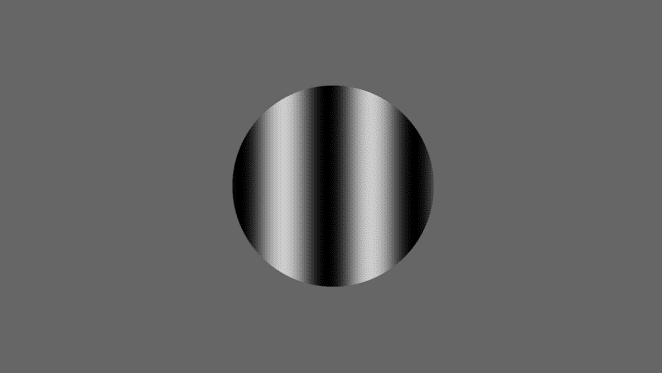
\includegraphics[width=4cm,height=4cm,keepaspectratio]{Figures/4.Chapter/tuning.png} \caption{tuning example.} \end{figure}

\subsection{Surround Modulation stimuli}
\label{subsec:subcsectionC}

Finally, for the SM protocol the frequencies of $0.04 /º$ and $1 s$ were chosen based on previous reports of largest V1 stimulation [REFERENCES]. The light contrasts of the gratings went from $0$ at dark to $122.5$ at background and $255$ at the lightest. Each trial had $2 s$, with $0.5 s$ of baseline, $1 s$ of stimuli display and $0.5 s$ of ITI. 

There were 124 possible trial types, repeated 20 times, to a total of 2480 trials in an 1 hour and 23 minutes session.

 \begin{table}[H]
\begin{center}\par
\scalebox{0.85}{
\begin{tabular}{c|cccccccccccccccccccccccccc}
\hline 
 
    
\multicolumn{1}{c}{Feature} & Value \\
           
           \hline
           \hline

\multicolumn{1}{c}{spatial frequency (/º)} & 0.04 \\
\multicolumn{1}{c}{temporal frequency (Hz)} & 1 \\

\multicolumn{1}{c}{central radius (º)} & 15 \\
\multicolumn{1}{c}{surround inner and outer radius (º)} & [27 50] \\
\multicolumn{1}{c}{stim directions (º)} & [0 90 180 270] \\
\multicolumn{1}{c}{dark, stim, background light} & [0 255 122.5] \\
\multicolumn{1}{c}{groups of stimuli} & C, S1, S1+C, S2, S2+C \\
\hline
        
\end{tabular}}
 \caption{Configurations regarding the SM protocol stimuli properties.}
    \vspace{-5mm}
    \label{table:SM}
\end{center}
\end{table}

There were 5 possible patches: a central one and four surround patches in the cardinal positions. The central patch was a circle of 15º radius, as the others were limited by an external circumference of 50º, an inner circumference of 27º (to obtain a 12º gap between the center and the surround patches) and the curresponding bissectors of the screen. For any patch, there were 4 available directions of gratings movement ($0º$, $90º$, $180º$ and $270º$).

With these patches, five groups of stimuli types were used:
\begin{itemize}
\item $C$ - only the center patch, in any of the 4 directions of movement (4 types);

\begin{figure}[h]\centering 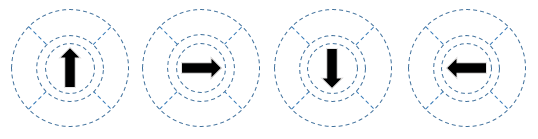
\includegraphics[width=9cm,height=9cm,keepaspectratio]{Figures/4.Chapter/C.PNG} \caption{Diagram of stimuli group C.} \end{figure}

\item $S1$ - only one surround patch, in any of the 4 cardinal top, bottom, left or right locations (S1T, S1B, S1L, S1R), and in any of the 4 directions (16 types);

\begin{figure}[h]\centering 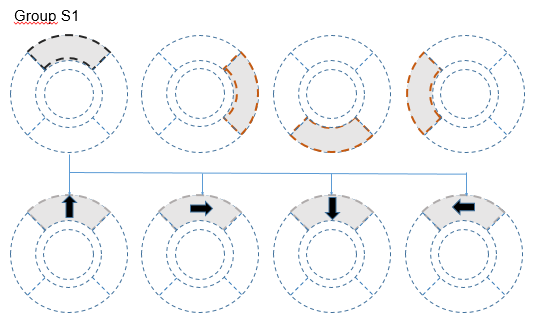
\includegraphics[width=9cm,height=9cm,keepaspectratio]{Figures/4.Chapter/S1.PNG} \caption{Diagram of stimuli group S1.} \end{figure}

\item $S1+C$ - One surround patch and the center patch, at any location of the surround($S1T+C$, $S1B+C$, $S1L+C$, $S1R+C$) and any direction for the center and for the surround (64 types);

\begin{figure}[H] \centering 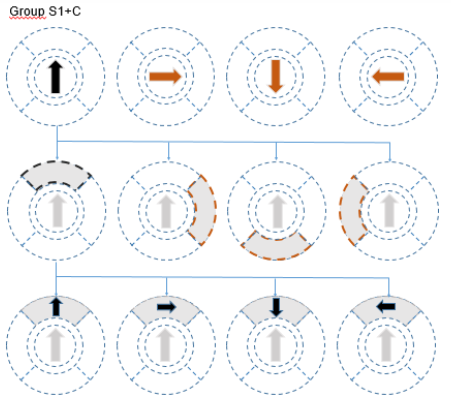
\includegraphics[width=9cm,height=9cm,keepaspectratio]{Figures/4.Chapter/S1C.PNG} \caption{Diagram of stimuli group S1C.} \end{figure}

\item $S2$ - only two surround patches, in opposite cardinal locations, either in the horizontal line ($S2H$) or the vertical line ($S2V$), both of them with gratings moving in the same of any of the 4 directions (8 types);

\begin{figure}[H] \centering 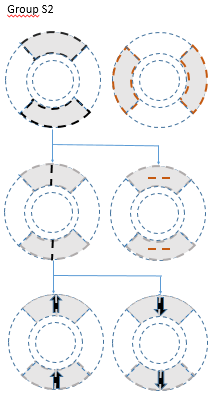
\includegraphics[width=8cm,height=8cm,keepaspectratio]{Figures/4.Chapter/S2.PNG} \caption{Diagram of stimuli group S2.} \end{figure}

\item $S2+C$ - Two surround patches and the center patch, both surround patches either in the horizontal ($S2H+C$) or the vertical line ($S2V+C$), both with gratings moving in the same of the possible directions and the center patch with gratings moving in any direction, not necessarily being the same from the surround stimuli (32 types).

\begin{figure}[H] \centering 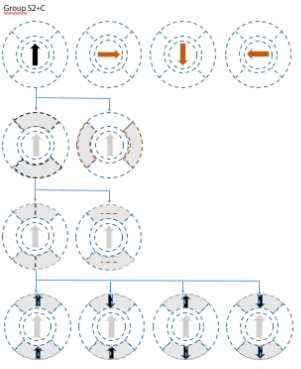
\includegraphics[width=10cm,height=10cm,keepaspectratio]{Figures/4.Chapter/S2C.PNG} \caption{Diagram of stimuli group S2C.} \end{figure}

\end{itemize}


\begin{figure}[H] \centering 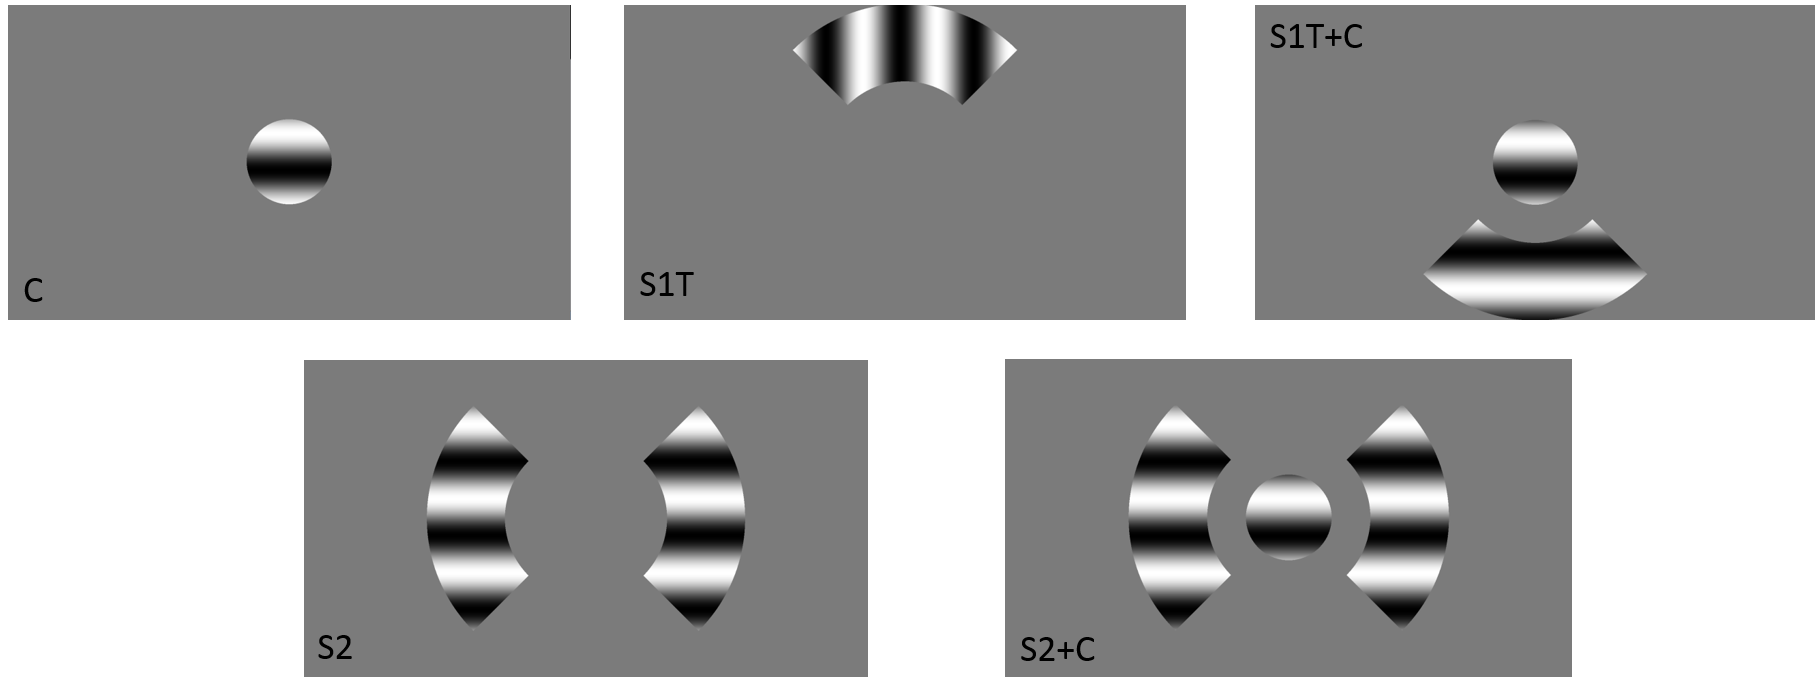
\includegraphics[width=12cm,height=12cm,keepaspectratio]{Figures/4.Chapter/SM.png} \caption{SM examples.} \end{figure}

Group $C$ was used as a more specific confirmation for the receptive field findings: here the stimuli was now in the center of the screen with the selected size for the analysis. Groups $S1$ and $S2$ provided the data that allowed to exclude from the analysis the cells that responded to stimulation in the defined surround. These had a receptive field that overlapped what we regarded as the surround and thus did not meet the criteria for investigating surround modulation effects in this experiment's designed manner. With the cells that did respond to group $C$ but did not to group $S1$ nor $S2$, we could then regard the effects of actual surround stimulation by examinating the responses to stimuli in the groups $S1+C$ and $S2+C$.
\cleardoublepage
% %%%%%%%%%%%%%%%%%%%%%%%%%%%%%%%%%%%%%%%%%%%%%%%%%%%%%%%%%%%%%%%%%%%%%%
% Dummy Chapter:
% %%%%%%%%%%%%%%%%%%%%%%%%%%%%%%%%%%%%%%%%%%%%%%%%%%%%%%%%%%%%%%%%%%%%%%

% %%%%%%%%%%%%%%%%%%%%%%%%%%%%%%%%%%%%%%%%%%%%%%%%%%%%%%%%%%%%%%%%%%%%%%
% The Introduction:
% %%%%%%%%%%%%%%%%%%%%%%%%%%%%%%%%%%%%%%%%%%%%%%%%%%%%%%%%%%%%%%%%%%%%%%
\chapter{Analysis}
\label{cap:Analysis}

\textit{Upon the experimental procedures, a developed pipeline was followed for the analysis of the RF, tuning and SM protocols, for each animal and imaging session. This process will be described hereby, along with the explanation of each utilized tool, analysis scripts and software. This chapter will first summarize the registration method utilized, the regions of interest selection technique, as well as the subsequent data treatment. In particular, for this project's experiments' analysis, Suit2p software for automated selection of neurons in a raw image and corresponding fluorescence traces extraction was implemented. The then also describe the RF analysis methods, followed by the tuning and finalize with some considerations on the SM analysis.
The statistical tools also used in the analysis are described in appendix chapter \ref{chapter:StatisticalTests}. }

\section{Experiment's outputs}
\label{sec:Experimentsoutputs}

Once an experiment is completed, a set of raw images, as well as the corresponding stimuli information and event timings is available. For each protocol, there is a set of frames for every trial, according to the TPLSM system's scanning speed of $30 Hz$ ($6 Hz$ per plane). 
For instance, the RF protocol comprises 1120 trials and the triggers sent from bpod to the imaging computer for separating the movies come at each 4 trials. There are thus, for this case, 280 sets of images. Since each trial endures for $1s$, each of these sets contains 6 frames for each of the 4 relevant planes, prefacing, for the RF protocol, 24 total frames per trial. In turn, each of these frames contains a $512 \times 512$ pixels image of the fluorescent signals emitted from the animal's brain ($200 \mu m \times 200 \mu m$) and detected at that time (figure \ref{cm006}, for an example).
For each of the trial's sets of images, there is the corresponding stimulus information being saved in a Matlab structure: In the case of the RF, the changing feature is the position and the gratings direction order of the stimulus patch being presented in the screen during that trial, for the Tuning protocol these are the spacial and temporal frequencies as well as the direction of the centred stimulus, and finally for the SM protocol the independent variable is the stimulus type number. Apart from these, the constant features of the stimuli at each protocol are also saved in the same stimuli structure. 
The trial time stamps in bpod's triggering, states and Psychtoolbox's clocked timings from a received trigger to the next are also saved. This allows, in the latter analysis, to confirm and correct the stimuli information in the case of any eventual skipped trials.
Finally, Scan Image configurations are also saved, in each trial's video header, keeping the information required about the laser's power during that experiment, multiplane settings and read brightness offsets.

\begin{figure}[H] \centering 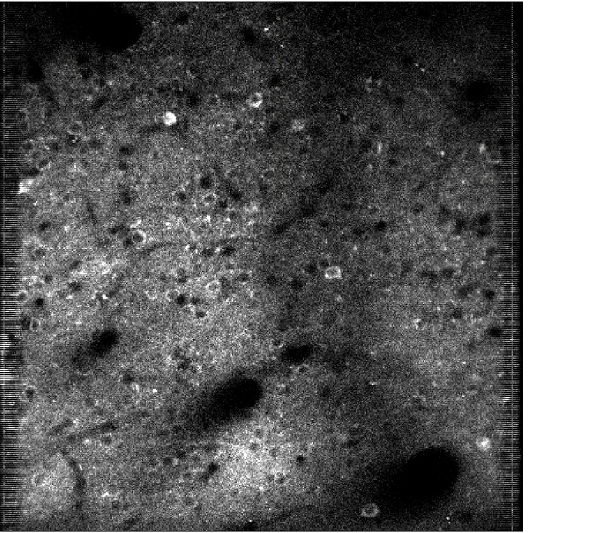
\includegraphics[width=10cm,height=10cm,keepaspectratio]{Figures/7.Results/ftraces/CM006.png} 
\caption{Average image of an example plane of imaging recordings across a session from an example animal. The full image corresponds to a $512\times 512$ map of $400 \mu m \times 400 \mu m$ of mouse V1 area, chosen as to respond to the center of the visual field of view.
\label{cm006}}
\end{figure}
\section{Images pre-processing: Separating planes and registration}
\label{sec:PreProcessing}

Each imaging raw movie intertwines the frames of each of the 4 planes. We used a software developed in the cortical circuits laboratory that parses and enables manipulations and sorting of these movies, across each trial or across each session, through an interactive GUI.

Loading a set of images from the middle of the session to this analyzer GUI, the first step is to project each of its frames in average images per plane. This creates four image averages (one per plane) over those movie frames which clean some of the noise inherent to those trials' acquisition.

These images will then be used, for each plane, as target images in the \textit{registration} phase. This stage is processed in iterative steps:

First, the user chooses a subset of movies around the firstly selected and averaged middle session movie - in this case, 15 movies are initially selected. Then, these movies are registered: The spatial correlations of each of the selected movies frames with the corresponding averaged images are computed. These are then used to correct for spatial shifts in the movies coming from drift while imaging or vascular micromovements, by minimizing the found phase correlations between the target image brightness values in $(x,y)$ and the brightness values at each position of each movie frame in the 2D plane. A relative translative offtset is estimated to best describe the relation between the two images.

Specifically, this phase correlation relies on a spatial frequency description of the data, calculated by fast Fourier transforms (FT). First, a window is selected to minimize edge effects, then the 2D Fourier transform of both images is calculated, as well as the cross-power spectrum $R$ that describes the distribution of power of the signal in different spatial frequency components:

\begin{equation}
\vec{G}_i = F (g_i(x,y)), G_{target}=F(g_{target}(x,y)) 
\end{equation}

and, with $\circ$ standing as pairwise multiplication:

\begin{equation}
R= \dfrac{\vec{G}_i \circ \vec{G}_{target}^*}{|\vec{G}_i \circ \vec{G}_{target}^*|}
\end{equation}

for each $i$ movie frame, $\vec{G}_i$ being the FT of the $g_i$ brightness function of that movie, and $\vec{G}_{target}$, $g_{target}$ respectively the FT and the brightness function of the target image of the respective plane.

Applying the inverse Fourier transform onto this spectrum then amounts to the normalized cross-correlation function. The peak value of this cross-correlation will be at the coordinates of the estimated shift, and can be found by an interpolation method.

When corrected, this amounts to a new averaged image across the selected and drift-corrected 15 movies. The process is then iteratively repeated, with respectively 25, 50, 100 and finally the full session of movies. These quantities were empirically choosed, as proven sufficient for good registration results in these experimental settings.

This registration ultimately produced full session image averages of the corrected image sets, as well as the transformations to impose on each of the image sets in order to achieve registered, well anchored movies for every plane.

\section{Suit2p pipeline}
\label{sec:Suit2ppipeline}

%You will need to analyze imaging data from large numbers of neurons. You will first need to identify  the cells in the images and extract their fluorescence traces. We have our own code, but you might use something like this:

The recordings from two-photon microscopy and calcium indicators yield the observation of large neuron populations' activity that must be processed in a suitable way to extract neuron's fluorescence traces. This data comprises multi-plane movies of a great number of cells, depending on the imaged region. Computational methods for its treatment should be not only accurate, but fast, as to grant the feasibility of substantial data's processing. 
\\In this project, the \textit{Suite2p} pipeline was used. This set of algorithms implements four modular processing independent steps: Image registration from raw movies through time and spatial phase correlation, the detection of regions of interest (ROIs), their interactive labelling and quality control and finally the extraction of a single representative fluorescence signal for each ROI.

The first stage of Suit2p is image registration, spatially aligning images taken at different times or from different viewpoints. This step from the algorithm was not used, as it was found to not perform as well as the iterative registration method described above for our data set. 

In much similiarity, the algorithm receives raw movies as inputs and corrects for the effects of brain movement. 
This registration is also based on finding a correlation-peak between a frame and a target image with a fast fourier transform, determining its offset, and applying the appropriate shift by means of FFT-based interpolation.
Additionally, to emphasize high-frequency content such as somata calcium-filled cellular compartments that could be dominated over in the previous scheme, the algorithm uses phase correlation, firstly spatially whitening the images - decorrelating the spatial information and leaving it with variance one - and then computing its correlation-maps. Sub-pixel shifts are also detected and corrected by an extension of this principle.
Non-rigid and rotation alignments are also made possible, by means of a generated globally non-rigid transformation. [TAKE THIS OUT]

The second stage uses the aligned movies and selects spatial regions of interest (ROIs) - somata, dendrites, spines or butons - with each pixel assigned to a positive weight. The model assumes the origin of the recorded signal in each pixel to be coming from three possible origins: the actual ROIs, measurement noise, but also from the neuropil - synaptically dense regions, out-of-focus dendrites and axons whose average activity contaminates the detection with a large and diffuse signal. 

To account for this important effect, the neuropil signal is represented in a set of spatially-localized basis functions \textbf{B}, covering the full field of view and each pixel \textit{k}. In each basis function j, the neuropil signal is a smooth timecourse $\vec{n}_{j}(t)$. Assuming the ROI signals to also be spatially localized, and having that, for each ROI i, its pixels all follow the same time course $\vec{f}_i(t)$ which is scaled by a constant positive factor, given by a sparse matrix $\Lambda _{ki}$ that is null if the pixel k does not belong to the ROI i. Finally, the noise is taken to be Gaussian and described by $\vec{\eta} _k(t) \sim N(0, \sigma ^2)$. We obtain the final model for the recorded signal $\vec{r}_k$(t) at pixel k:

\begin{equation}
    \vec{r}_k(t)=\sum_i \Lambda _{ki} \vec{f}_i (t) + \sum _j B_{kj} \vec{n}_j(t) + \vec{\eta}_k(t)
\end{equation}

This model is thereupon fitted to the data, by iterations of ROI detection (finding new sources), activity extractions (re-estimating time courses and neuropil contribution) and pixel-reassignments (taking into account the other ROIs, reestimating a given ROI spatial distribution).

The third stage amounts to the quality control of the classification, distinguishing between cell and non-cell (compartments, such as dendrites or axons), and lowering the fluorescence variance in each ROI. This is firstly done by an automated classifier and then curated by the used through the software's GUI that displays an improved resolution image, each ROIs information,  and allows its relabelling as cell/non-cell. One of the great advantages of this pipeline is that the selection-stage improves with use and training of the classifier. The implemented classifier is based on a set of $k$ feature statistics $r_k(n)$ computed for each ROI $n$ (encompassing both activity and shape parameters). The distributions of these features are estimated by human-labelled data and then fed to a Bayes classifier that is trained to reproduce them. The classifiers' cell $p^+_k(x)$ versus non-cell $p^-_k(x)$ smoothed empirical distributions for each statistic $x$ are then applied to new data cells. A new ROI N is classified by comparing every combined statistics' cell score $\prod_k p^+_k(r_k(N))$ with its non-cell score $\prod_k p^-_k(r_k(N))$, and labelling it cell or no-cell according to the category that results in the highest score for that ROI.

\begin{figure}[H] \centering 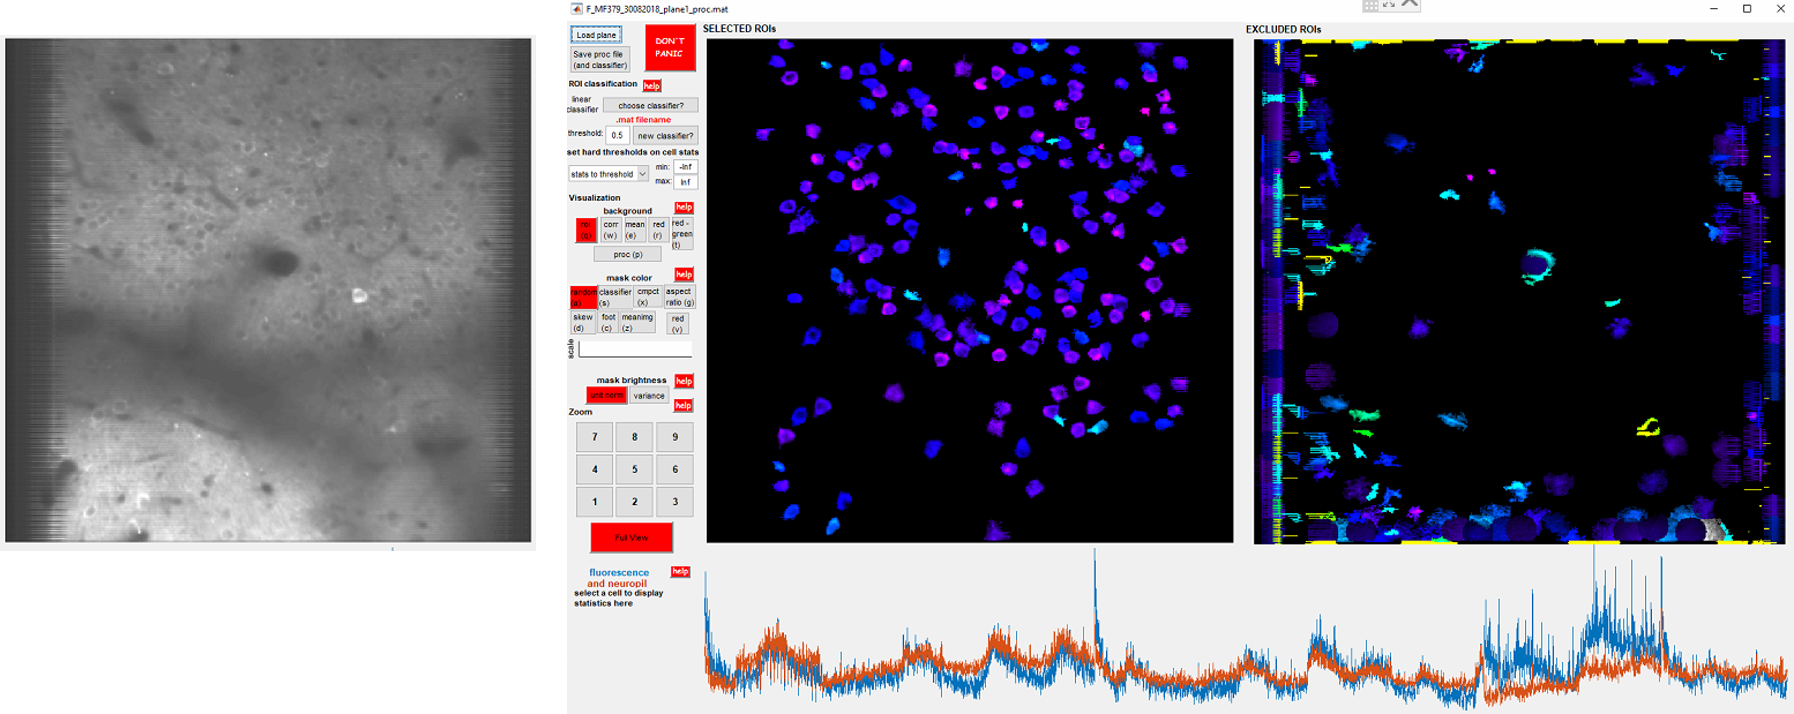
\includegraphics[width=13cm,height=13cm,keepaspectratio]{Figures/7.Results/ftraces/suit2p.png} 
%\caption{6_popPlots_Animal2_Session6} 
\end{figure}

Finally, the fourth stage of the pipeline outputs, for each ROI, a single calcium fluorescence time-varying signal. Again, this signal is corrected for the neuropil contamination signals. Furthermore, the spike train - the action potential sequence - that causes this signal is estimated, by use of a fitting model. 
A model is used for the uncorrected fluorescence $\vec{F}_i$, with a contribution by the convolution of the spike train $\vec{s}_i \geq 0$ with the calcium response kernel $\vec{k}_i$, a scalled neuropil and the noise:

\begin{equation}
    \vec{F}_i(t) = [\vec{s}_i * \vec{k}_i](t) + c_i \vec{N}_i (t) + noise
\end{equation}

To fit this model, $\vec{F}_i$ is extracted for each ROI i, the neuropil trace $\vec{N}_i$ is computed by averaging pixels in a ring shaped region around the ROI, and finally the coefficient $c_i$ and the spike train $\vec{s}_i$ are estimated for each cell by optimization of the cost function:

\begin{equation}
    Cost(\vec{s}_i, c_i)=||\vec{F}_i - \vec{s}_i * \vec{k}_i - c_i \cdot \vec{N}_i|| ^2 + \lambda \cdot L(\vec{s}_i)
\end{equation}

with $L(\vec{s}_i)$ a continuous, non-negative possible penalty on the spike train for each ROI.

In this way, the \textit{Suit2p} treatment of the raw movies produces a neuropil-corrected calcium trace $\vec{F}_i - c_i \vec{N}_i$, as well as the spike times estimates $\vec{s}_i$.

This processed data of fluorescence traces will be the substance for the posterior analysis.
\section{Data treatment}
\label{sec:DataTreatment}

Having the extracted neuropil corrected fluorescence traces, F, for all of the session's time, it is also required to extract $\Delta F/F$ traces: these indicate the measured changes in fluorescence between the cell's peak stimulation times and resting state and serve as the actual data measurements to use in all of subsequent analysis.

For every ROI's trace response, the baseline fluorescence ($F_0$) was estimated by discarding the tails of the fluorescence trace distribution and taking the mean fluorescence, using a 60 s sliding window. The obtained value was then used to calculate $\Delta F/F$ traces ($\dfrac{F-F_0}{F_0}$) for each cell (figure \ref{dfoverf}, left).

Cell  $\Delta F/F$ responses are thus mostly distributed around zero, with positive tails corresponding to spike responses (for an example cell $\Delta F/F$ distribution, figure \ref{dfoverf}, right).


\begin{figure}[H] \centering 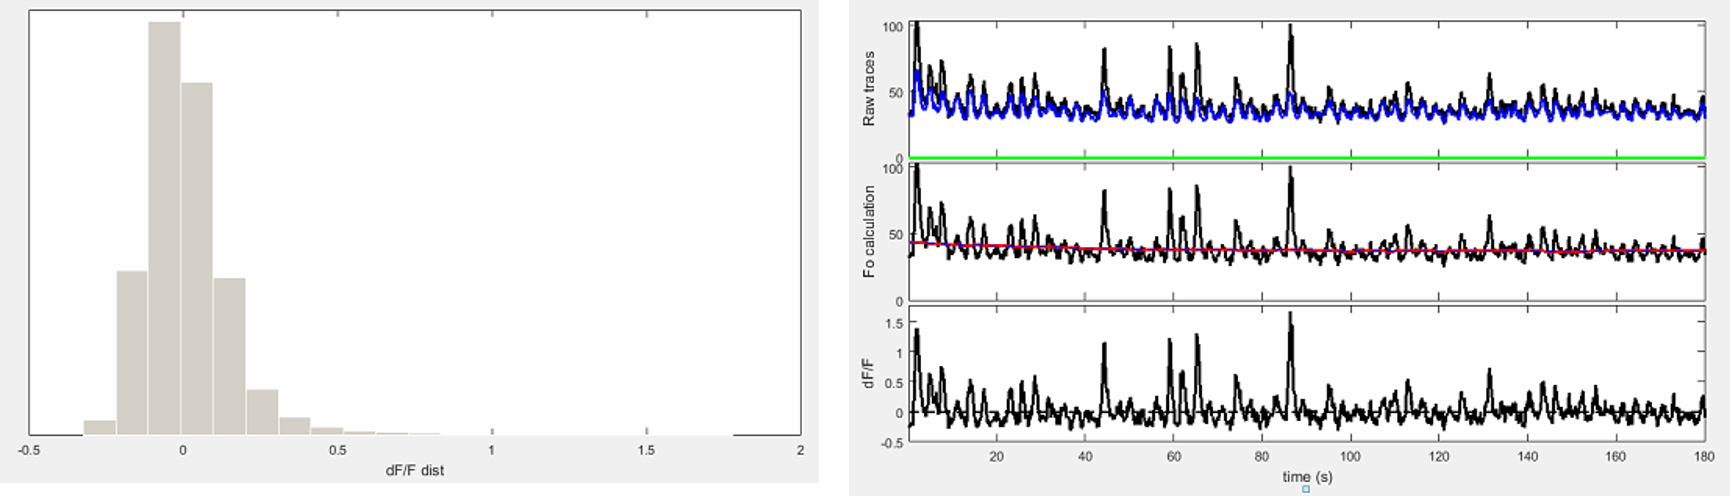
\includegraphics[width=15cm,height=15cm,keepaspectratio]{Figures/7.Results/ftraces/dFoverF.png} 
\caption{$\Delta F/F$ computation and results for an example ROI.
\newline \textbf{Left:} \textbf{Top} First 3 minutes section of raw fluorescence trace, F, for the example ROI (black trace) superimposed with the fluorescence baseline estimation trace for that ROI done by using a 60 s sliding window to discard trace's tails (blue trace); \textbf{Middle} Same fluorescence trace (black trace) superimposed with the baseline estimation value, $F_0$ (red trace), calculated as the average result of the baseline estimation trace in the top panel's blue trace, over the full session; \textbf{Bottom} $\Delta F/F$, computed as $\dfrac{F-F_0}{F_0}$.
\newline \textbf{Right:} Example ROI's $\Delta F/F$ distribution histogram. Cell's responses are mostly distributed around zero, with positive tails corresponding to spike responses.
\label{dfoverf}}
\end{figure}

Reviewing the process, we start with intrisic optical imaging on the subjects, to assess each animal's retinotopy maps and find the corresponding center field of view V1 encoding locations. 

We use two-photon imaging at that found location (with more thorough search for the center locations with the tuning protocol), and acquire brain recording sets of images of that brain's location GCaMP6s activity-related fluorescence values, for 4 different depth planes, while the subjects are shown stimuli (RF, tuning and SM protocols). 

These extracted raw images are then registered, and run through Suit2p pipeline, to select ROIs according to pixels temporal and spacial correlations in the image. These ROIs' pixels' fluorescence levels are averaged over that region and neuropil corrected. This results in raw fluorescence traces over the session's time.

With these, $\Delta F/F$ responses are computed. These are the processed data to map to the presented stimuli and use in the following analysis.

\section{RF analysis}

At each session's end, a RF analysis was held to assess whether the V1 imaged position corresponded to neurons with RFs centred in the center of the visual field, as these were the fixed intended positions for the subsequent SM spatial structure analysis.

Responses of each ROI were baseline subtracted and analysed trial by trial, mapping each trial's response to the visual field position that the corresponding stimulus was presented at (figure \ref{rfanalysis}, left panels).

Then, these responses were averaged over repetition trials, portraying mean response levels for each of the visual field positions (figure \ref{rfanalysis}, middle panels).

Finally, normalized gray-scale maps were produced for the response maps $R(az, el)$, with $az$ and $el$ the azimuth and elevation retinotopic coordinates, averaging over time on each of the positions' mean trace responses (figure \ref{rfanalysis}, right panels).

\begin{figure}[H] \centering 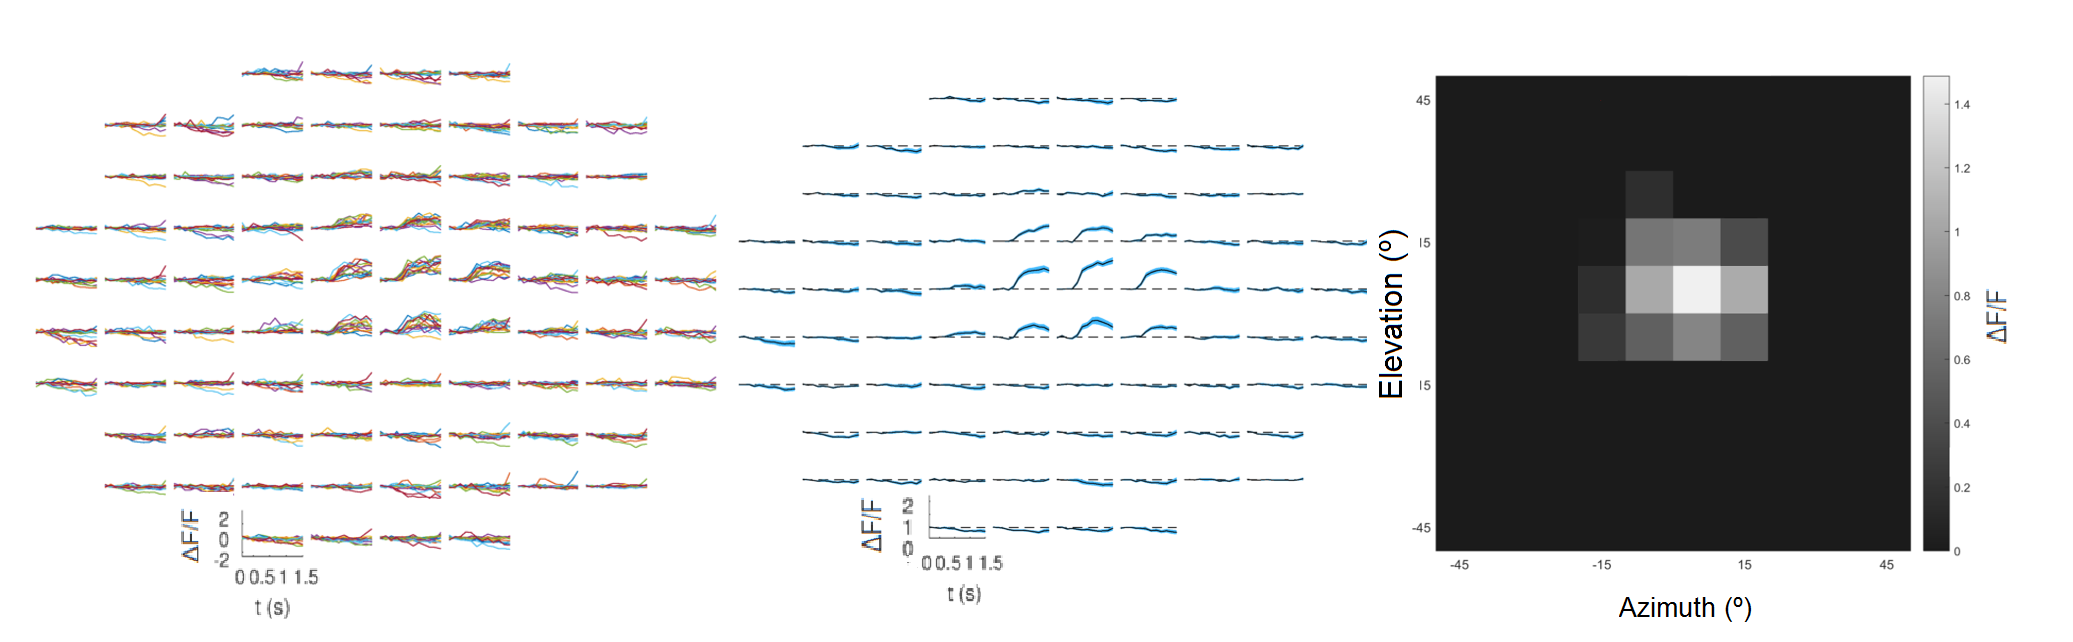
\includegraphics[width=16.2cm,height=16.2cm,keepaspectratio]{Figures/7.Results/rf/rf1.png} 
\caption{Example cell with well centred RF. 
\newline \textbf{Left:} Individual traces. Each of the 14 trial-type repetition trace response is represented in a different colour, for each of the visual field stimulated region. 
\newline \textbf{Middle:} Mean traces. Average traces over the 14 repetitions, represented also for each azimuth and elevation center stimulus condition. 
\newline \textbf{Right:}RF map. Response strengths to each of the stimulus positions, in a gray-scaled colour map.}
\label{rfanalysis}
\end{figure}

Each of these neurons' response maps was fitted to 2D-Gaussian ellipses, using Matlab implementation of the least-squares Levenberg-Marquardt algorithm (as in \cite{Marques2018}):

\begin{dmath}
R(az,el)=a+b\times \exp \left[ - \left( \dfrac{az-az_0}\times \cos(\theta)+ el-el_0)\times \sin(\theta){\sqrt{2} \times \sigma_1}\right)^2 - \left( \dfrac{-(az-az_0) \times sin \theta + (el-el_0)\times \cos(\theta)}{\sqrt{2} \times \sigma_2}\right)^2\right]
\end{dmath}

with $(az_0, el_0)$ the 2D Gaussian center coordinates, $\sigma_1$ and $\sigma_2$ the standard deviations of the gaussian across the two dimensions, $\theta$ the rotation angle between the gaussian and the $(az,el)$ axis, $a$ an offset parameter and $b$ an amplitude parameter.

The RF was then defined as the ellipse centred at $(az_0, ele_0)$ and limited by the standard deviations  ($\sigma_1$, $\sigma_2$):

\begin{equation}
\left[ \left( \dfrac{(az-az_0)\cdot \cos(\theta) + (el-el_0)\cdot \sin(\theta)}{\sigma_1}\right)^2 + \left(\dfrac{-(az-az_0)\cdot \sin(\theta) + (el-el_0)\cdot \cos(\theta)}{\sigma_2}\right)^2\right]=1
\end{equation}

The subsequent analysis was restricted to fits with $R^2>0.5$, as lower values corresponded to RF unreliable estimations. Within 10 sessions with 4 planes each, across 4 animals, 3168 out of 4198 dataset ROIs ($75\%$) were considered.

Analysing plane by plane, for each animal and session (example planes in figure \ref{ellipses}), one could assess that most of the considered RF centres were placed with similar centres within the retinotopical space, as theoretically expected for the short distances of $200 \times 200) \mu m$ imaged V1 planes. 

Two of the sessions showed very high elevation RFs, and were thus discarded for subsequent analysis, leaving 2772 measured RF cells and a total of 3728 cells ($74\%$ fitted RFs) to be analysed in regards to SM effects.

\begin{figure}[H] \centering 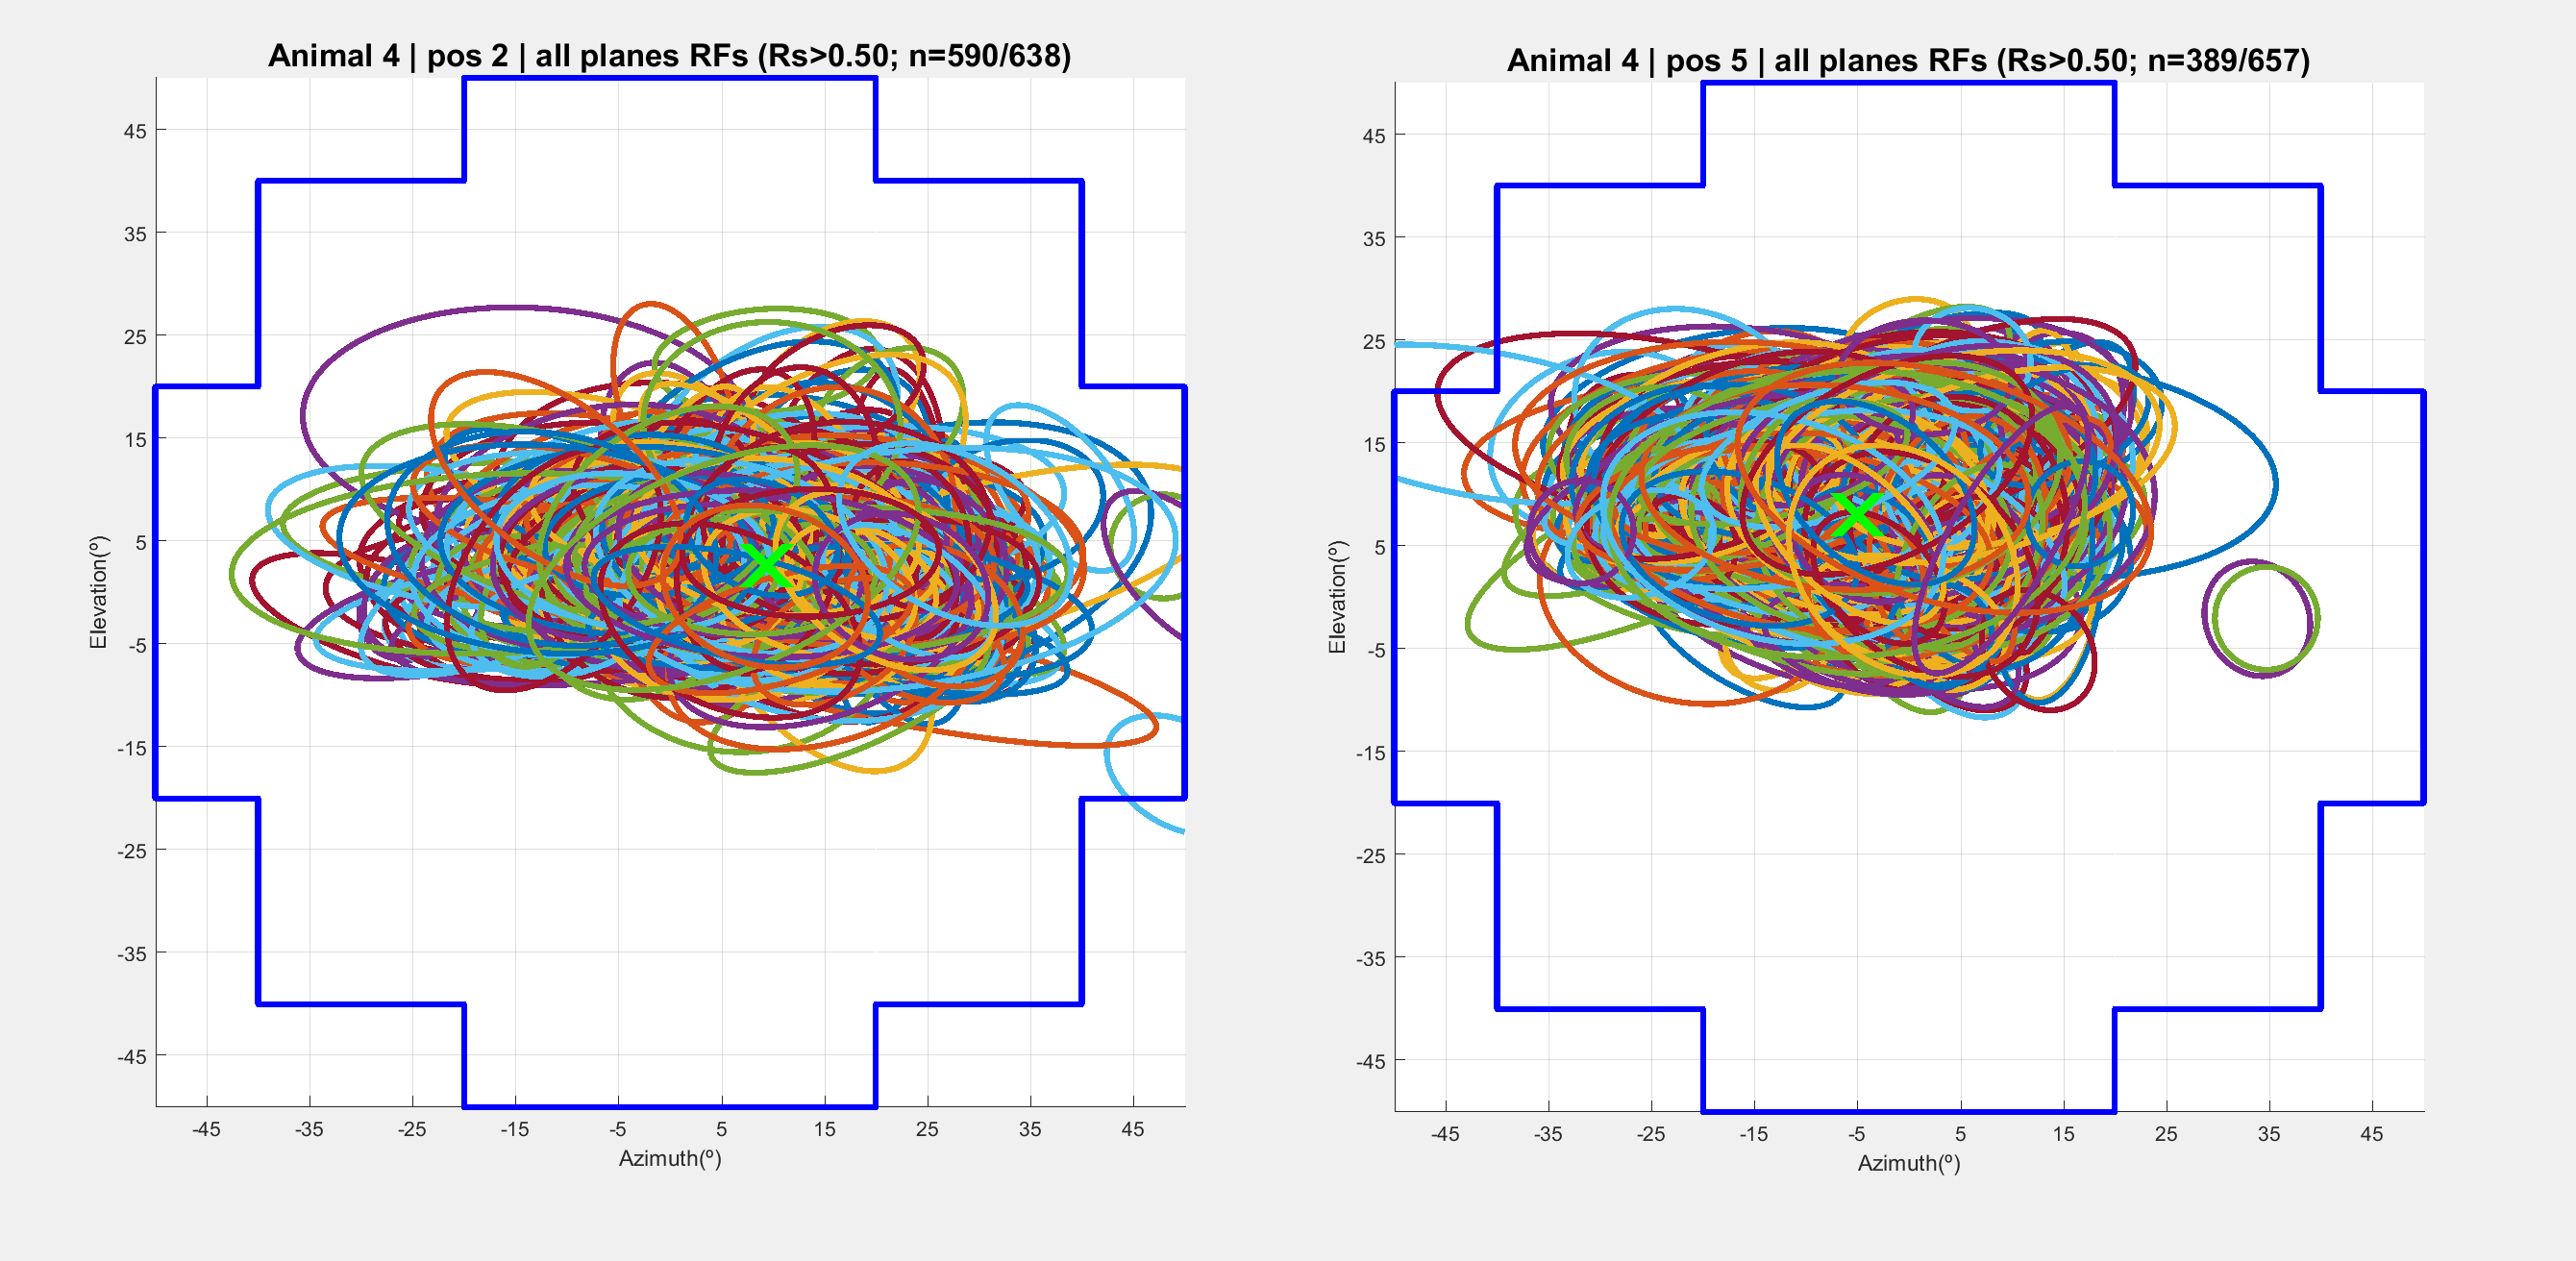
\includegraphics[width=13cm,height=13cm,keepaspectratio]{Figures/7.Results/rf/ellipsesAnimal4pos2andpos5.png} 
\caption{Superimposed 2D gaussian ellipsoidal fits for each neuron in the same plane. Two planes from two different sessions with the same animal are presented as examples.}
\label{ellipses}
\end{figure}

\section{Tuning analysis}
\label{tuningresults}

To validate bpod's tuning protocol, the selected neurons were analysed in regards to their direction (8 directions), spatial (2) and temporal (2) frequencies tuning selectivity.

Neurons in V1 can have orientation selectivity (\cite{Hubel1959}, \cite{Hubel1962}), that is, respond more strongly to a preferred orientation than to any other orientation. For mice, these orientation-selective (OS) cells are not organized into functional columns as they are for carnivores and primates (\cite{Hubel1962}), yet they do present strong orientation selectivity.

Moreover, a subset of  OS cells are also direction-selective (DS): these respond most strongly to a preferred direction than to any other.

For orientation analysis, responses of opposite directions are averaged together, and ploted on polar coordinates (figures \ref{tuninganalysisOS} and \ref{tuninganalysisDS}). The vector sum of responses at each individual trial (combining the trials for each of the same orientation opposed directions) then forms the \textit{orientation vector} of that trial. The orientation vectors for all trials then exhibit the cell's orientation tuning properties.
In the analogous way, for direction analysis, each trial measurement is binned to different direction labels, and the vector sum of the responses at individual directions then amounts to a direction vector for each trial. Direction vectors for all trials represent the cell's direction tuning properties.

Statistical significance is assessed with vector-based Hotelling's $t^2$-tests with confidence of 95\% in this project's case, to ask whether the 2D mean of the distribution of orientation and or direction vectors differ from (0,0).
 
 For any orientation, if the responses to a given orientation are significantly higher than responses to any other orientation, then the former is called the neuron's preferred orientation. This differential effect can be measured with an orientation selectivity index (OSI), for the preferred orientation response in the considered space. With  $R_{pref_or}$ the responses to the preferred orientation and $R_{orth}$ the responses to the orientation orthogonal to the preferred:
\begin{equation}
\text{OSI}= \dfrac{R_{pref \_or} - R_{orth}}{R_{pref \_or} + R_{orth}}
\end{equation}

Similarly, in the direction space, a preferred direction can also be determined for neurons that have significantly higher responses in one direction than they do in the null direction relative to the former. A DSI can be computed, for the direction doublet:

\begin{equation}
\text{DSI}=\dfrac{R_{pref} - R_{null}}{R_{pref} + R_{null}}
\end{equation}

In regards to the spatial and frequency tuning, here we used a restricted $(2 \times 2)$ space and found that for most cells, in this space, the preferred spatial frequency was of 0.04 cycles per degree and the preferred temporal frequency was at 1 Hz. These were the frequency specifications used in both the RF protocol and the SM protocol.

Here, we present two example cell responses for the different stimulus conditions in the tuning protocol: an OS cell (figure \ref{tuninganalysisOS}) and a DS cell (figure \ref{tuninganalysisDS}).

\begin{figure}[H] \centering 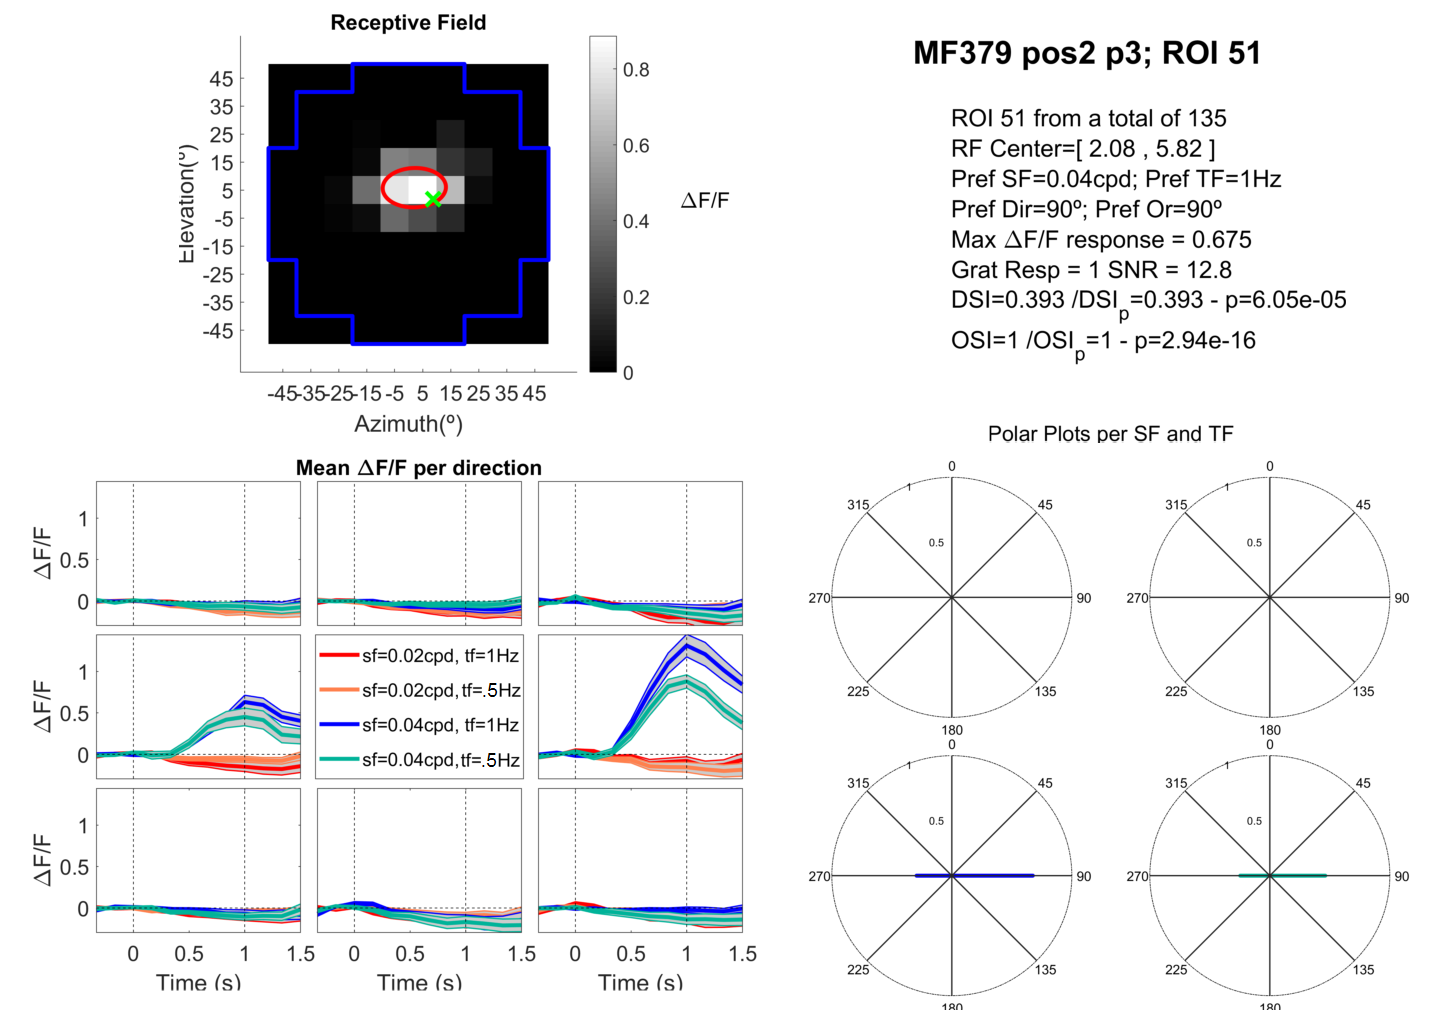
\includegraphics[width=12cm,height=12cm,keepaspectratio]{Figures/7.Results/tuning/MF379_pos2_p3_ROI0051.png} 
\caption{Tuning analysis for an example OS cell. Preferred $SF=0.04 cpd$, $TF=1 Hz$, up direction and vertical orientation. $DSI=1$ ($p=1.87 \cdot 10^{-5}$), $OSI=0.967$ ($p=3.4 \cdot 10^{-4}$).}
\label{tuninganalysisOS}
\end{figure}

\begin{figure}[H] \centering 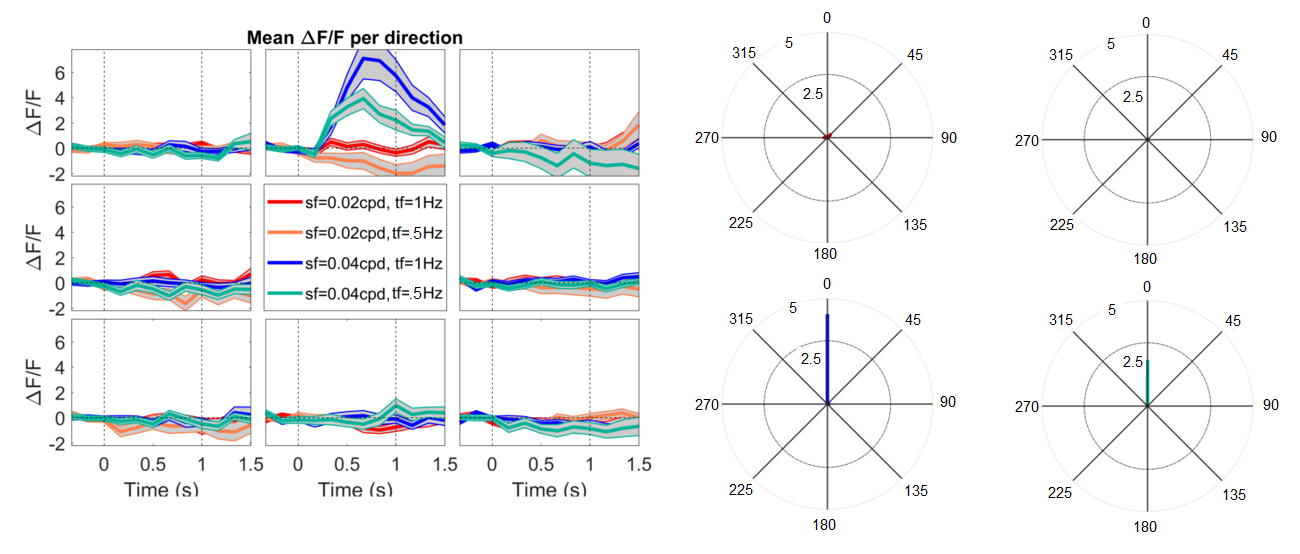
\includegraphics[width=12.5cm,height=12.5cm,keepaspectratio]{Figures/7.Results/tuning/CM006_pos1_p4_ROI0138.png} 
\caption{Tuning analysis for an example DS cell. Preferred $SF=0.04 cpd$, $TF=1 Hz$, temporal direction and horizontal orientation. DSI=0.393 ($p=6.05 \cdot 10^{-5}$), OSI=1 ($p=6.05 \cdot 10^{-5}$).}
\label{tuninganalysisDS}
\end{figure}

\subsection{Surround modulation analysis}
\label{cap:Methods}

SM analysis started with the mapping of responses during the protocol to corresponding stimuli types, from the 124 possible ones. During the experiments, 20 repetitions were held for most sessions. However, in the analysis, it was noticeable that responses decreased a lot in the second part of the protocol, possibly due to anaesthesia cumulative effects and/or adaptation to the stimuli. Therefore, to prevent from adding noise to averaged measurements, the subsequent analysis was using only the 10 first repetitions of each trial type.

Trial types were ordered in a given structure:

\begin{itemize}
\item \textbf{[1:4]} S1T, at the four directions (up, temporal, down, nasal); 
\item \textbf{[5:8]} C, analogous to above; 
\item \textbf{[9:12]} S1B, analogous to above;
\item \textbf{[13:16]} S1L, analogous to above;
\item \textbf{[17:20]} S1R, analogous to above; 
21:36 S1T+C, with first quarter (21:24) center up and surround in the 4 directions (up, temporal, down, nasal), second quarter (25:28) center temporal and surround in the 4 directions, third quarter (29:32) center down and surround in the 4 directions, and fourth quarter (33:36) center nasal and surround in the 4 directions;
\item \textbf{[37:52]} S1B+C, analogous to above;
\item \textbf{[53:68]} S1L+C, analogous to above;
\item \textbf{[69:84]} S1R+C, analogous to above;
\item \textbf{[85:100]} S2H+C, with first quarter (85:100) center up and the two horizontally positioned surrounds in the same of 4 directions (up, temporal, down, nasal), second quarter (89:92) center temporal and surrounds in the same of 4 directions, third quarter (93:96) center down and surrounds in the same of 4 directions, and fourth quarter (97:100) center nasal and surrounds in the the same of 4 directions;
\item \textbf{[101:104]} S2H, at the four directions (up, temporal, down, nasal);
\item \textbf{[105:120]} S2V+C, with first quarter (105:108) center up and the two vertically positioned surrounds in the same of 4 directions (up, temporal, down, nasal), second quarter (109:112) center temporal and surrounds in the same of 4 directions, third quarter (113:116) center down and surrounds in the same of 4 directions, and fourth quarter (117:120) center nasal and surrounds in the the same of 4 directions;
\item \textbf{[121:124]} S2V, at the four directions (up, temporal, down, nasal);
\end{itemize}
%\chapter{Statistical Tests}
\label{chapter:StatisticalTests}

Along the SM analysis, statistical tests were used to test given hypothesis, assess results significance and perform multiple comparisons. These tools were implemented with Matlab ingrained functions (\texttt{signtest}, \texttt{ranksum}, \texttt{anovan}, \texttt{corrcoef} and \texttt{regress}). Here we summarily review these tools and underlying mathematical basis.

\section{Two-sided sign-tests}
\label{subsec:signtests}

Sign-tests are nonparametric tests, for given independent observations, for the hypothesis that the difference between the correspondent variables has a given median value $\eta_0$. In this work's analysis, the hypothesized median was zero. 

In this test, the only assumption is that data is collected independently from a continuous distribution.

For a two-sided test, as used in this project's analysis, the null hypothesis and alternative hypothesis are given by:

H_0 : $\eta = \eta _0$

H_a : $\eta \neq \eta _0$

We define $S_1$ the counts of the number of observations less than $\eta _0$ and  $S_2$ the counts of the number of observations larger than $\eta _0$. 

The test statistic is the given by:

\begin{equation}
S=max(S_1, S_2)
\end{equation}

If the null hypothesis $H_0$ is true, then S follows a binomial distribution $S ~ \text{Binomial} (m, 0.5)$, with $m$ the number of observations, discarding the data points equal to $\eta _0$.

Then, in general, the p-value, \textit{p}, is defined by

\begin{equation}
p=2 \text{Pr}\left[ X \geq S \right]
\end{equation}

and we reject the null hypothesis $H_0$ if \textit{p} is smaller or equal to a given significance threshold $\alpha$.

For large samples, as is the case for this project's data sets, it can be shown that if X ~ Binomial (m, 0.5), then the distribution can be approximated by X ~ Normal (0.5m, 0.5(1-0.5)).

Then, the continuity corrected (replacing $S$ by $S-0.5$) z-statistic can be used:

\begin{equation}
Z=\dfrac{S-E(S)}{\sqrt{V(S)}}= \dfrac{(S-0.5m - 0.5 sign(n_+-n_-))}{\sqrt{(0.5)(0.5)m}}
\end{equation}

with $E(S)$ and $V(S)$ respectively the expected value and the variance, ($V(S)=E(S^2)-(E(S))^2$)of the random variable S, m the number of elements, $n_{+}$ and $n_{-}$ respectively the number of positive and negative differences from the hypothesized median value.

This statistic follows a normal distribution Z~Norm(0, 1), if the null hypothesis is true. 

The p-value can thus be defined, for large data sets:

\begin{equation}
p = 2 \text{Pr}\left[X \geq Z\right]
\end{equation}

and we again reject the null hypothesis $H_0$ if \textit{p} is smaller or equal to a considered significance threshold $\alpha$.

\section{Wilcoxon signed rank-sum tests}
\label{subsec:subbsectionC}

Wilcoxon signed rank-sum tests are non-parametric tests used when collected data samples $(y_{11},...,y_{n1})$ and $(y_{12},...,y_{n2})$ is expected to be dependent, that is, data is \textit{paired}.

As for the last test, the only assumption here is that data is collected independently from a continuous distribution.

Fist, for the n sized data set, we compute the within-individual differences, for $i=1,...,n$, $x_i = y_{i1} - y_{i2}$ and discard any data point for which $x_i=0$, adjusting the sample size - let's call it $m$.

Then, the absolute values of $x_1,...,x_m$ are sorted into ascending order, and labelled with a rank from 1 to $m$. In the case of ties, average ranks are given.

Next, we define two rank sums:

$T_+ =$ Sum of ranks for which $x_i>0$

$T_-$ = Sum of ranks for which $x_i<0$

The null hypothesis is then posed:

\begin{center}
$H_0$: No change between the two measurements
\end{center} 

and put against three alternative hypothesis: $H_a(1)$ significant decrease, $H_a(2)$ significant increase and $H_a(3)$ significant change between the two measurements.

Critical $T_0$ values are tabled. If $T_- \leq T_0$, we reject $H_0$ in favour of $H_a(1)$; if $T_+ \leq T_0$, we reject $H_0$ in favour of $H_a(2)$; and finally, with a two-sided test with $T=min(T_-, T_+)$, if  $T \leq T_0$, we reject $H_0$ in favour of $H_a(3)$.

For large sample tests, as is the case, the algorithm uses a Z statistic:

\begin{equation}
Z = \dfrac{T_+ - \dfrac{m(m+1)}{4}}{\sqrt{\dfrac{n(m+1)(2m+1)}{24}}}
\end{equation}

If $H_0$ is true, Z can be approximated by a normal distribution Z ~ Normal(0,1), with different tabled critical values for each of the alternative hypothesis tested with.

In Matlab's algorithm, continuity correction and tie adjustments are also used, and the tests are carried in an analogous way.

\section{N-way analysis of variance}
\label{subsec:subcsectionC}

An n-way analysis of variance (ANOVA) is an extension on the one-way ANOVA. This conservative statistical tool examines the effect of n categorical independent variables on one continuous dependent variable. This results in not only an estimation of each categorical variable's influence but also assesses the influence of the interactions between these variables.

A n-way ANOVA determines if a data set differs as a function of groups of n factors. A n-way ANOVA can be generalized from a two-way ANOVA. For 3 factors A, B and C, for example, a model can be written as:

\begin{equation}
y_{ijkr}=\mu + \alpha_i + \beta_j + \gamma_k +(\alpha \beta)_{ij}+(\beta \gamma)_{jk}+(\alpha \beta \gamma)_{ijk}+\epsilon_{ijkr}
\end{equation}

with $y_{ijkr}$, an observation of the response variable; $i$, $j$ and $k$ representing respectively groups from factors A, B and C and r the replication number; $\mu$ the overall mean; $\alpha_i$, $\beta_j$ and $\gamma_k$ respectively the deviations of groups of factor A, B or C from $\mu$ due to corresponding factors A, B or C. $\epsilon_{ijkr}$ are the random disturbances, assumed independent, normally distributed and with constant variance. The 2-way and 3-way interactions between factors are accounted for in the model, within the other terms of the model equation, respectively with two subscripts and three subscripts.

A n-way ANOVA the tests 7 null versus alternative hypothesis:

The hypothesis about the equality of the mean response for groups of factor A, with I the number of groups in A:

\begin{center}
$H_0=: \alpha_1=\alpha_2...=\alpha_I$

$H_a:$ at least one $\alpha_i$ is different, $i=1,...,I$
\end{center}

and the equivalent analogous for factors B and C.

The two-factors interaction hypothesis:

\begin{center}

$H_0$:$(\alpha \beta)_{ij}=0$

$H_a$: at least one$(\alpha \beta)_{ij}\neq 0$

\end{center}

and the equivalent analogous for other two-factor interactions.

Finally, the three-factor interaction hypothesis:

\begin{center}
$H_0$:$(\alpha \beta \gamma)_{ijk}=0$

$H_a$: at least one$(\alpha \beta \gamma)_{ijk}\neq 0$
\end{center}

\section{Pearson correlation coefficients}
\label{subsec:subcsectionC}

Correlation coefficients between two random variables A and B measure their linear dependence. For N scalar observations from each variable, the Pearson correlation coefficient is given by:

\begin{equation}
\rho(A, B) = \dfrac{1}{N-1} \sum_{i=1}^N \left( \dfrac{A_i - \mu _A}{\sigma _A}\right) \left( \dfrac{B_i - \mu_B}{\sigma _B}\right)
\end{equation}

with $\mu_A$ and $\sigma_A$ the mean and standard deviation of A, and $\mu_A$ and $\sigma_A$ the mean and standard deviation of B.

In matlab's algorithm, matrices of correlation coefficients are computed and the matrix of p-values for testing the null hypothesis that there is no relationship between the observed phenomena. If these p-values are smaller than the considered $\alpha$ threshold, the correlations are deemed significant.

\section{Multiple linear regression}
\label{subsec:subcsectionC}

Linear regression models describe the relationship between a dependent variable $y$, and $K$ independent variable(s) $X$.

A multiple linear regression model is given, for $i=1,...,n$, with n the number of responses, by:

\begin{equation}
y_i=\beta_0 + \beta_1 X_{i1}+...+\beta_p X_{ip}+\epsilon_i
\end{equation}

with $y_i$ the $ith$ response, $\beta_k$ the $k$th coefficient, $X_{ij}$ the \textit{i}th observation on the \textit{j}th independent variable, with $j=1,...,k$, and $\epsilon_i$ the random error term, assumed uncorrelated, independent and identically normal distributed. 

It follows that the fitted linear function is given, for $i=1, ..., n$ by:

\begin{equation}
\hat{y_i}= \sum _{k=0}^K b_k f_k(X_{i1},...X{ip})
\end{equation}

with $f$ a scalar-valued function of the independent variables, and K the number of independent variables.
\section{Permutation test}

When interested on strong null hypothesis, permutation tests can be conducted for assessing sampling distributions. This test builds sampling distributions by resampling the observed data. This is done with no replacement, by simply eliminating the outcome labels on the original sample data and then randomly redistributing the observed values under those same labels. This shuffling process can be repeated to obtain a large number of resamples.
Significance tests can then be used for the null hypothesis that these resample distributions do not differ from the original distribution.

\section{Multivariate comparisons: Holm-Bonferroni method}

Finally, in this work, many comparisons were held on different pools of the dataset. For this reason, the multiple comparisons problem needs to be accounted for: The more statistical inferences that are made simultaneously, the more likely it is for Type I error (false positive) inferences to be made. This issue steams from considering an overall confidence level for the whole set of simultaneous tests, while these threshold levels are to be considered individually. The controlled variable should be the familywise error rate (FWER), the probability of making one or more type-I errors, with a given significance level threshold, $FWER \leq \alpha$.

To compensate for this problem in the multivariate comparisons held, the Holm-Bonferroni method was used to adjust the rejection thresholds for each individual tested hypotheses. 

With $H_1,...,H_m$ a family of $m$ null hypothesis, and $p_1,...,p_m$ the corresponding p-values, we order the p values from lowest to highest $p_{(1)},...,p_{(m)}$, associated to the respective null hypothesis, $H_{(1)},...,H_{(m)}$.

For an established $\alpha$ significance level threshold, we let $k$ be the minimal index such that $P_{(k)}> \dfrac{\alpha}{m+1-k}$. Then, we reject the null hypothesis $H_{(1)}...H_{(k-1)}$. If $k=1$, no null hypothesis is rejected, and if no such $k$ exists, all null hypothesis are rejected. This method ensures that $FWER \leq \alpha$ has intended to appropriately assess the joint multiple inferences.
%\cleardoublepage
% %%%%%%%%%%%%%%%%%%%%%%%%%%%%%%%%%%%%%%%%%%%%%%%%%%%%%%%%%%%%%%%%%%%%%%
% Dummy Chapter:
% %%%%%%%%%%%%%%%%%%%%%%%%%%%%%%%%%%%%%%%%%%%%%%%%%%%%%%%%%%%%%%%%%%%%%%

% %%%%%%%%%%%%%%%%%%%%%%%%%%%%%%%%%%%%%%%%%%%%%%%%%%%%%%%%%%%%%%%%%%%%%%
% The Introduction:
% %%%%%%%%%%%%%%%%%%%%%%%%%%%%%%%%%%%%%%%%%%%%%%%%%%%%%%%%%%%%%%%%%%%%%%
\fancychapter{Results}
\label{cap:Results}

\textit{Present the chapter content.}

\section{RF analysis}

At each session's end, a RF analysis was held to assess whether the V1 imaged position corresponded to neurons with RFs centred in the center of the visual field, as these were the fixed intended positions for the subsequent SM spatial structure analysis.

Responses of each ROI were baseline subtracted and analysed trial by trial, mapping each trial's response to the visual field position that the corresponding stimulus was presented at (figure \ref{rfanalysis}, left panels).

Then, these responses were averaged over repetition trials, portraying mean response levels for each of the visual field positions (figure \ref{rfanalysis}, middle panels).

Finally, normalized gray-scale maps were produced for the response maps $R(az, el)$, with $az$ and $el$ the azimuth and elevation retinotopic coordinates, averaging over time on each of the positions' mean trace responses (figure \ref{rfanalysis}, right panels).

\begin{figure}[H] \centering 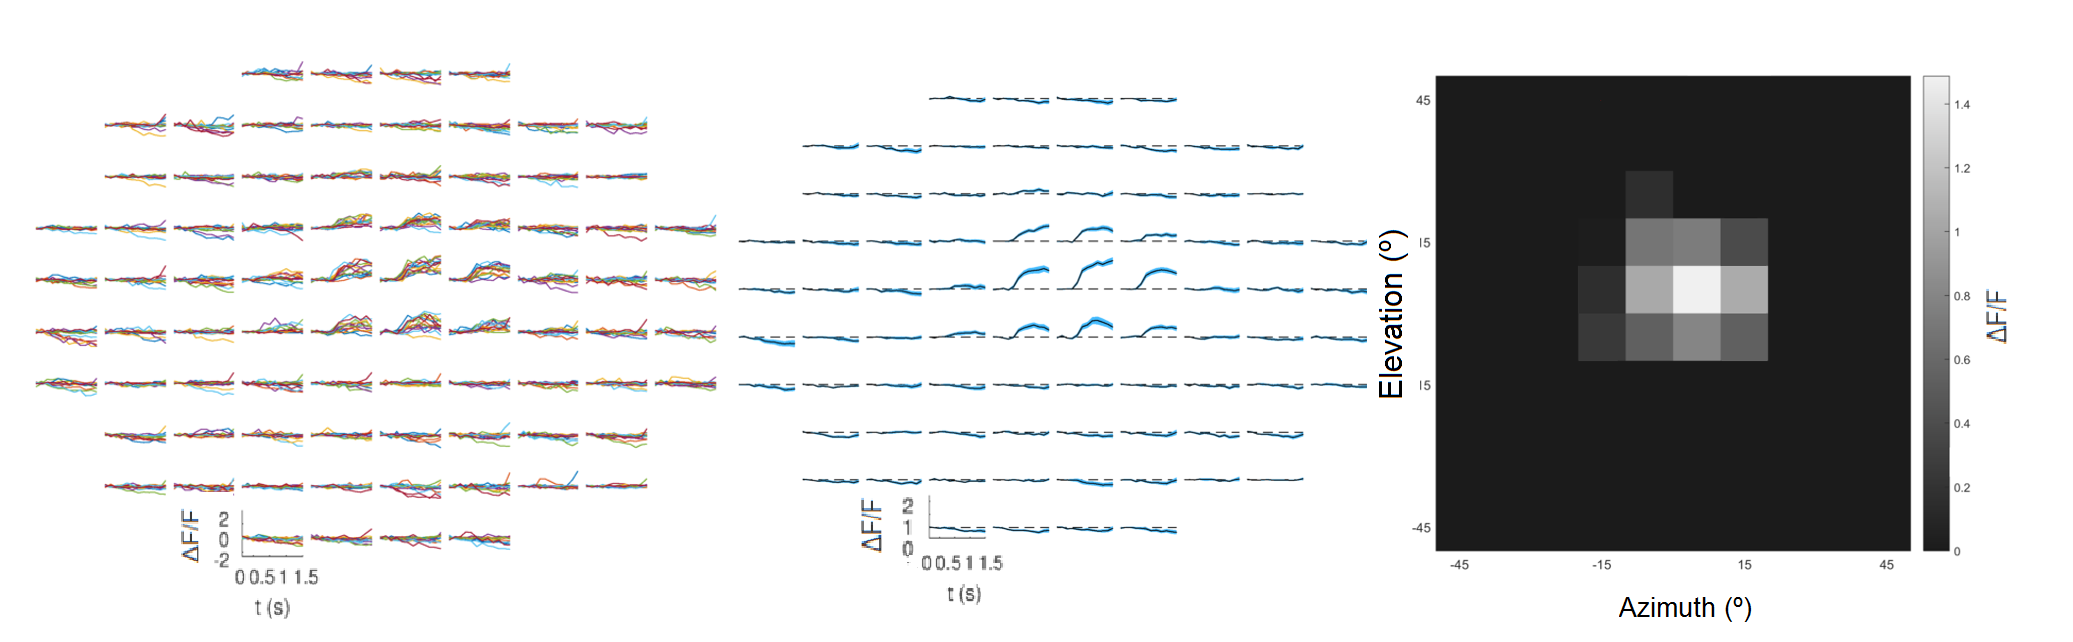
\includegraphics[width=13cm,height=13cm,keepaspectratio]{Figures/7.Results/rf/rf1.png} 
\caption{Example cell with well centred RF. 
\newline \textbf{Left:} Individual traces. Each of the 14 trial-type repetition trace response is represented in a different colour, for each of the visual field stimulated region. 
\newline \textbf{Middle:} Mean traces. Average traces over the 14 repetitions, represented also for each azimuth and elevation center stimulus condition. 
\newline \textbf{Right:}RF map. Response strengths to each of the stimulus positions, in a gray-scaled colour map.}
\label{rfanalysis}
\end{figure}

Each of these neurons' response maps was fitted to 2D-Gaussian ellipses, using Matlab implementation of the least-squares Levenberg-Marquardt algorithm (as in \cite{Marques2018}):

\begin{dmath}
R(az,el)=a+b\times \exp \left[ - \left( \dfrac{az-az_0}\times \cos(\theta)+ el-el_0)\times \sin(\theta){\sqrt{2} \times \sigma_1}\right)^2 - \left( \dfrac{-(az-az_0) \times sin \theta + (el-el_0)\times \cos(\theta)}{\sqrt{2} \times \sigma_2}\right)^2\right]
\end{dmath}

with $(az_0, el_0)$ the 2D Gaussian center coordinates, $\sigma_1$ and $\sigma_2$ the standard deviations of the gaussian across the two dimensions, $\theta$ the rotation angle between the gaussian and the $(az,el)$ axis, $a$ an offset parameter and $b$ an amplitude parameter.

The RF was then defined as the ellipse centred at $(az_0, ele_0)$ and limited by the standard deviations  ($\sigma_1$, $\sigma_2$):

\begin{equation}
\left[ \left( \dfrac{(az-az_0)\cdot \cos(\theta) + (el-el_0)\cdot \sin(\theta)}{\sigma_1}\right)^2 + \left(\dfrac{-(az-az_0)\cdot \sin(\theta) + (el-el_0)\cdot \cos(\theta)}{\sigma_2}\right)^2\right]=1
\end{equation}

The subsequent analysis was restricted to fits with $R^2>0.5$, as lower values corresponded to RF unreliable estimations. Within 10 sessions with 4 planes each, across 4 animals, 3168 out of 4198 dataset ROIs ($75\%$) were considered.

Analysing plane by plane, for each animal and session (example planes in figure \ref{ellipses}), one could assess that most of the considered RF centres were placed with similar centres within the retinotopical space, as theoretically expected for the short distances of $200 \times 200) \mu m$ imaged V1 planes. 

Two of the sessions showed very high elevation RFs, and were thus discarded for subsequent analysis, leaving 2772 measured RF cells and a total of 3728 cells ($74\%$ fitted RFs) to be analysed in regards to SM effects.

\begin{figure}[H] \centering 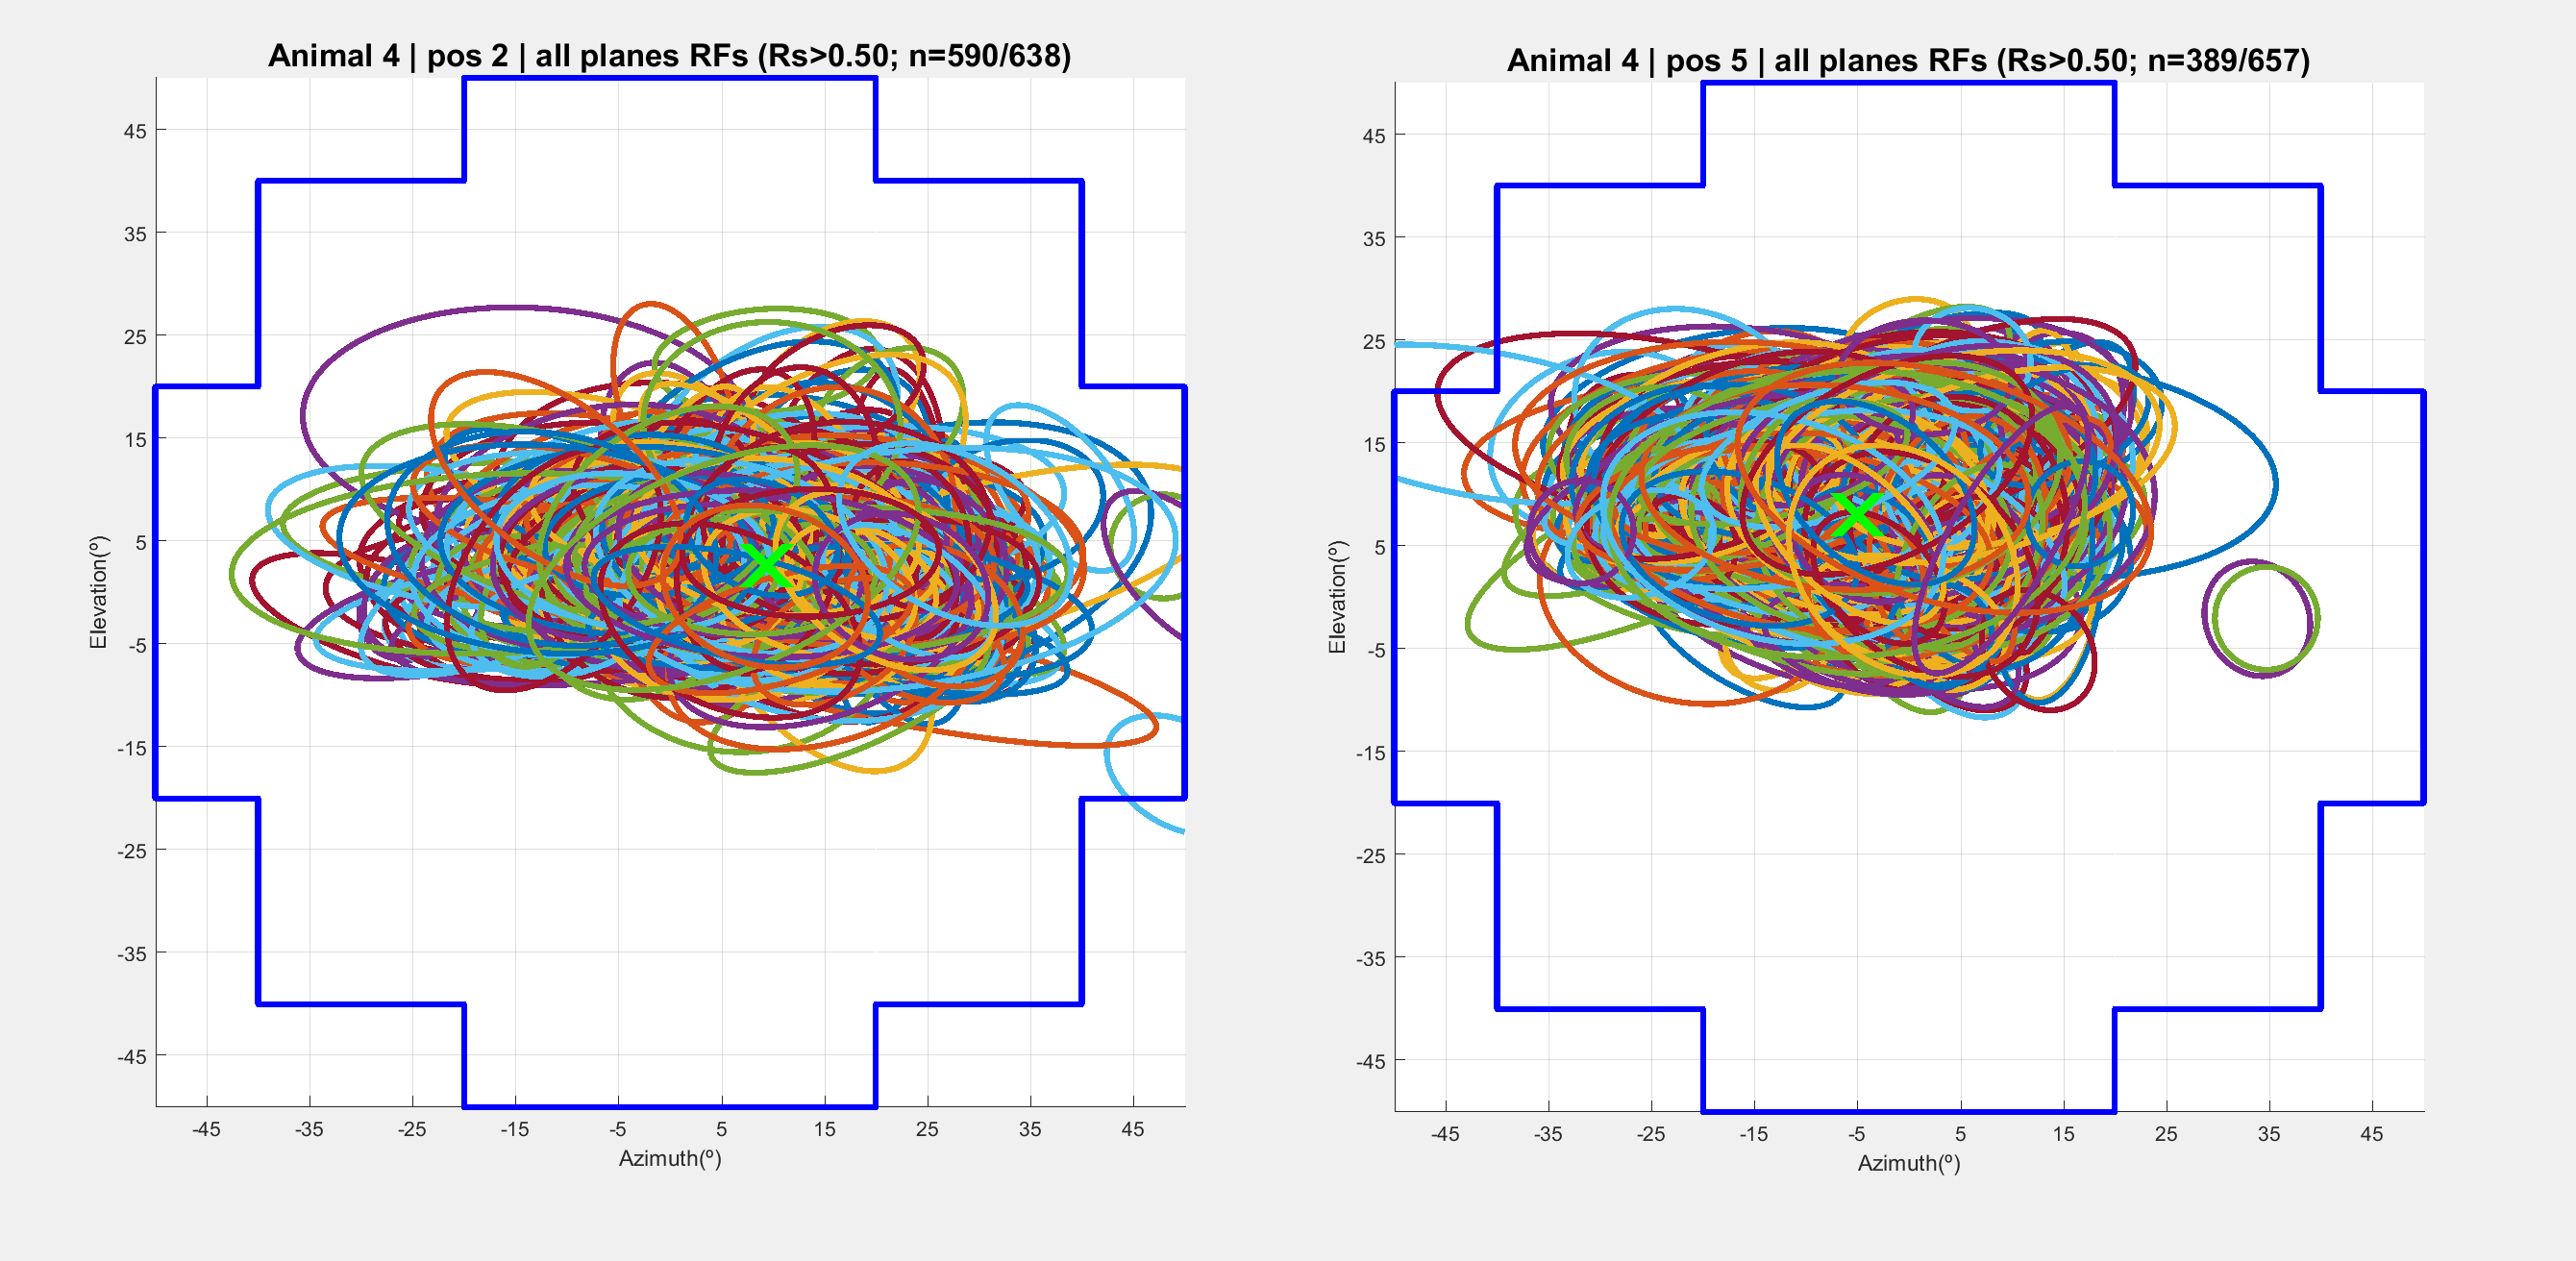
\includegraphics[width=13cm,height=13cm,keepaspectratio]{Figures/7.Results/rf/ellipsesAnimal4pos2andpos5.png} 
\caption{Superimposed 2D gaussian ellipsoidal fits for each neuron in the same plane. Two planes from two different sessions with the same animal are presented as examples.}
\label{ellipses}
\end{figure}

\section{Tuning analysis}
\label{tuningresults}

To validate bpod's tuning protocol, the selected neurons were analysed in regards to their direction (8 directions), spatial (2) and temporal (2) frequencies tuning selectivity.

Neurons in V1 can have orientation selectivity (\cite{Hubel1959}, \cite{Hubel1962}), that is, respond more strongly to a preferred orientation than to any other orientation. For mice, these orientation-selective (OS) cells are not organized into functional columns as they are for carnivores and primates (\cite{Hubel1962}, \cite{Hubel1968}), yet they do present strong orientation selectivity (\cite{Girman1999}, \cite{Ohki2005}). 

Moreover, a subset of  OS cells are also direction-selective (DS): these respond most strongly to a preferred direction than to any other.

For orientation analysis, responses of opposite directions are averaged together, and ploted on polar coordinates (figures \ref{tuninganalysisOS} and \ref{tuninganalysisDS}). The vector sum of responses at each individual trial (combining the trials for each of the same orientation opposed directions) then forms the \textit{orientation vector} of that trial. The orientation vectors for all trials then exhibit the cell's orientation tuning properties.
In the analogous way, for direction analysis, each trial measurement is binned to different direction labels, and the vector sum of the responses at individual directions then amounts to a direction vector for each trial. Direction vectors for all trials represent the cell's direction tuning properties.

Statistical significance is assessed with vector-based Hotelling's $t^2$-tests with confidence of 95\% in this project's case, as suggested by examinations in \cite{Mazurek2014}, to ask whether the 2D mean of the distribution of orientation and or direction vectors differ from (0,0).
 
 For any orientation, if the responses to a given orientation are significantly higher than responses to any other orientation, then the former is called the neuron's preferred orientation. This differential effect can be measured with an orientation selectivity index (OSI), for the preferred orientation response in the considered space. With  $R_{pref_or}$ the responses to the preferred orientation and $R_{orth}$ the responses to the orientation orthogonal to the preferred:
\begin{equation}
\text{OSI}= \dfrac{R_{pref \_or} - R_{orth}}{R_{pref \_or} + R_{orth}}
\end{equation}

Similarly, in the direction space, a preferred direction can also be determined for neurons that have significantly higher responses in one direction than they do in the null direction relative to the former. A DSI can be computed, for the direction doublet:

\begin{equation}
\text{DSI}=\dfrac{R_{pref} - R_{null}}{R_{pref} + R_{null}}
\end{equation}

In regards to the spatial and frequency tuning, here we used a restricted $(2 \times 2)$ space and found as expected (\cite{Whichpapershowsthis?}) that for most cells, in this space, the preferred spatial frequency was of 0.04 cycles per degree and the preferred temporal frequency was at 1 Hz. These were the frequency specifications used in both the RF protocol and the SM protocol.

Here, we present two example cell responses for the different stimulus conditions in the tuning protocol: an OS cell (figure \ref{tuninganalysisOS}) and a DS cell (figure \ref{tuninganalysisDS}).

\begin{figure}[H] \centering 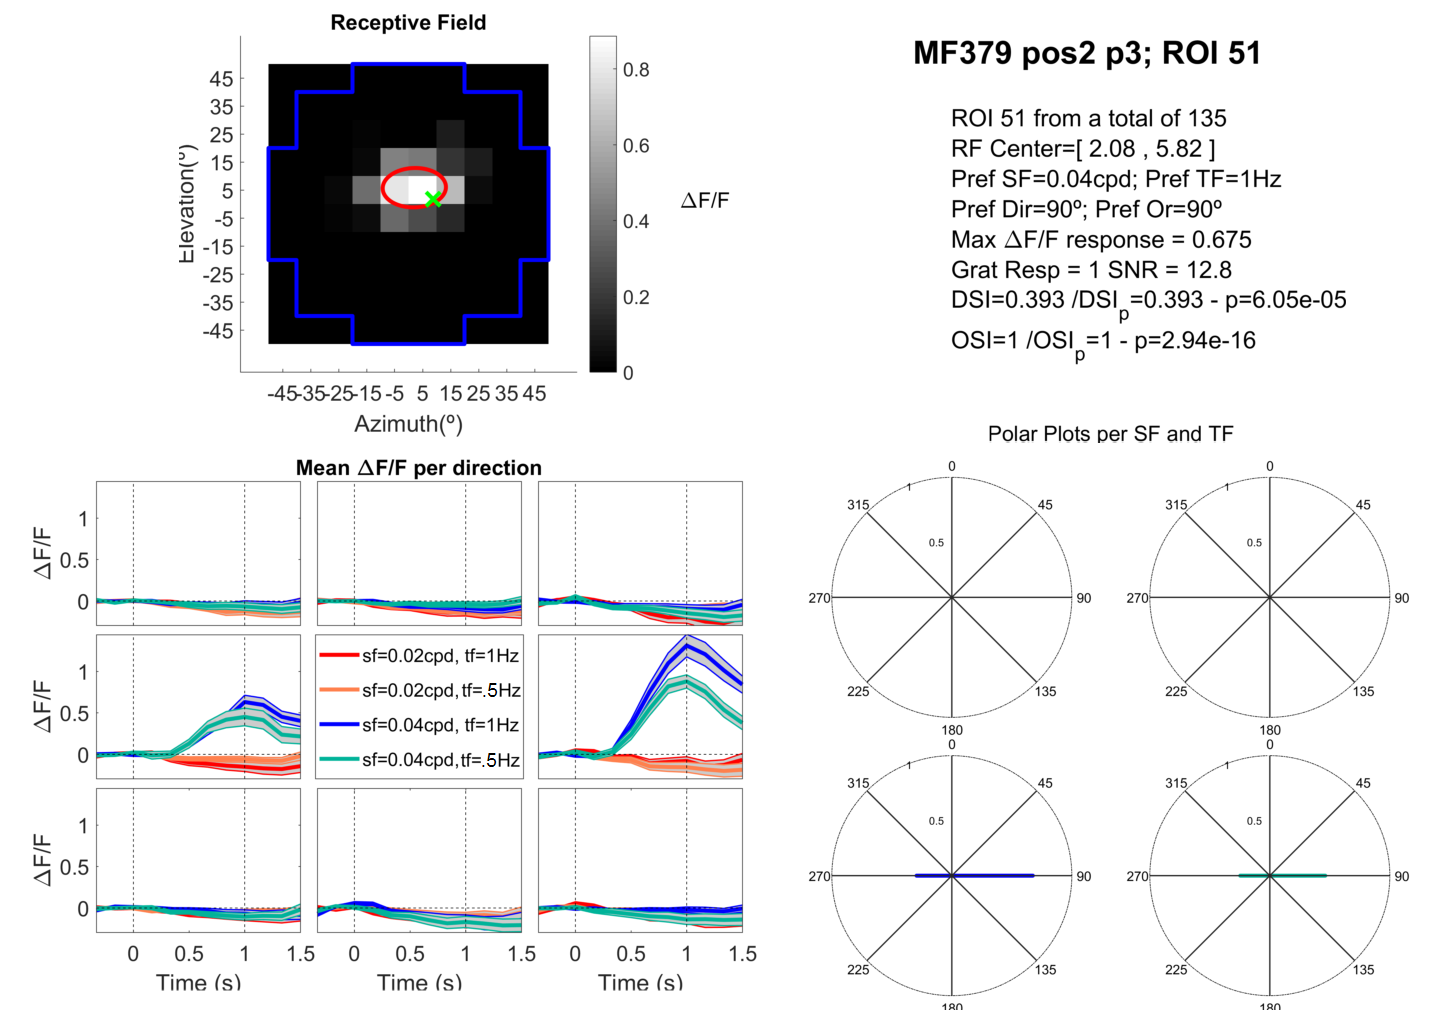
\includegraphics[width=12cm,height=12cm,keepaspectratio]{Figures/7.Results/tuning/MF379_pos2_p3_ROI0051.png} 
\caption{Tuning analysis for an example OS cell. Preferred $SF=0.04 cpd$, $TF=1 Hz$, up direction and vertical orientation. $DSI=1$ ($p=1.87 \cdot 10^{-5}$), $OSI=0.967$ ($p=3.4 \cdot 10^{-4}$).}
\label{tuninganalysisOS}
\end{figure}

\begin{figure}[H] \centering 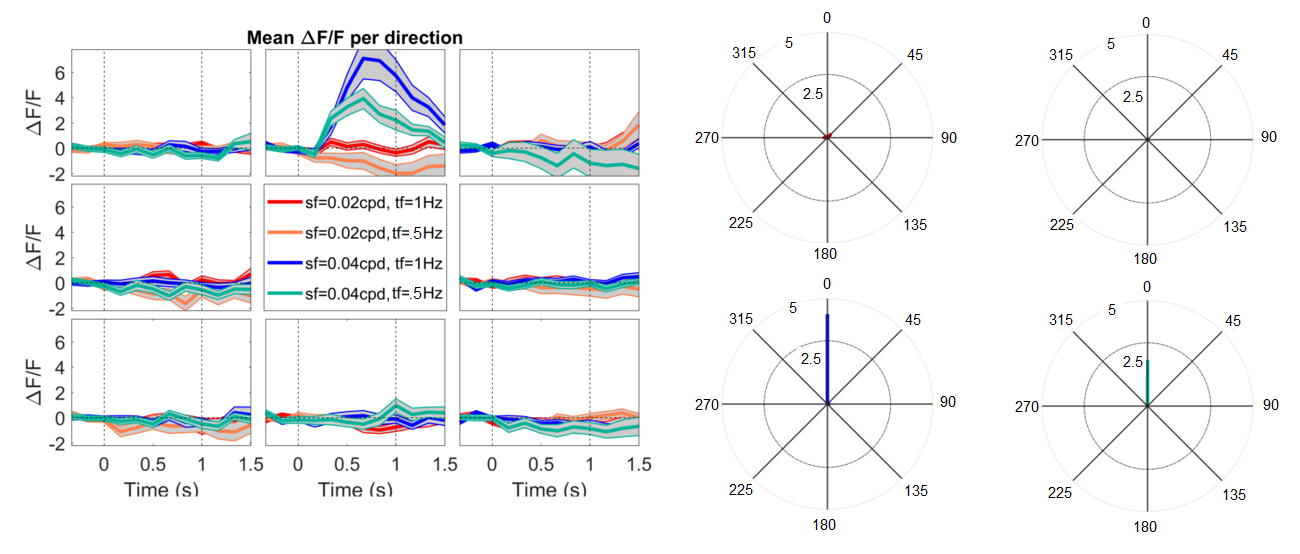
\includegraphics[width=12.5cm,height=12.5cm,keepaspectratio]{Figures/7.Results/tuning/CM006_pos1_p4_ROI0138.png} 
\caption{Tuning analysis for an example DS cell. Preferred $SF=0.04 cpd$, $TF=1 Hz$, temporal direction and horizontal orientation. DSI=0.393 ($p=6.05 \cdot 10^{-5}$), OSI=1 ($p=6.05 \cdot 10^{-5}$).}
\label{tuninganalysisDS}
\end{figure}

\section{SM analysis - individual cells}

SM analysis started with the mapping of responses during the protocol to corresponding stimuli types, from the 124 possible ones. During the experiments, 20 repetitions were held for most sessions. However, in the analysis, it was noticeable that responses [GET IMAGE] decreased a lot in the second part of the protocol, possibly due to anaesthesia cumulative effects and/or adaptation to the stimuli. Therefore, to prevent from adding noise to averaged measurements, the subsequent analysis was using only the 10 first repetitions of each trial type.

We start with individual cell example analysis, and present hereby two example cells' SM main effects.

\subsection{DS example cell}
\label{DSexamplecell}

We first consider, for simplification, a DS example cell: This cell only responds significantly to one of the four center directions used in this protocol.

Baseline-subtracted response strength for each trial by order of appearance can be plotted against time (stimulus onset at 0.5s), showing no visible structure (image \ref{individualDStrials}, left). 
Trials were then averaged by trial type and these were ordered in a given structure:

\begin{itemize}
\item \textbf{[1:4]} S1T, at the four directions (up, temporal, down, nasal); 
\item \textbf{[5:8]} C, analogous to above; 
\item \textbf{[9:12]} S1B, analogous to above;
\item \textbf{[13:16]} S1L, analogous to above;
\item \textbf{[17:20]} S1R, analogous to above; 
21:36 S1T+C, with first quarter (21:24) center up and surround in the 4 directions (up, temporal, down, nasal), second quarter (25:28) center temporal and surround in the 4 directions, third quarter (29:32) center down and surround in the 4 directions, and fourth quarter (33:36) center nasal and surround in the 4 directions;
\item \textbf{[37:52]} S1B+C, analogous to above;
\item \textbf{[53:68]} S1L+C, analogous to above;
\item \textbf{[69:84]} S1R+C, analogous to above;
\item \textbf{[85:100]} S2H+C, with first quarter (85:100) center up and the two horizontally positioned surrounds in the same of 4 directions (up, temporal, down, nasal), second quarter (89:92) center temporal and surrounds in the same of 4 directions, third quarter (93:96) center down and surrounds in the same of 4 directions, and fourth quarter (97:100) center nasal and surrounds in the the same of 4 directions;
\item \textbf{[101:104]} S2H, at the four directions (up, temporal, down, nasal);
\item \textbf{[105:120]} S2V+C, with first quarter (105:108) center up and the two vertically positioned surrounds in the same of 4 directions (up, temporal, down, nasal), second quarter (109:112) center temporal and surrounds in the same of 4 directions, third quarter (113:116) center down and surrounds in the same of 4 directions, and fourth quarter (117:120) center nasal and surrounds in the the same of 4 directions;
\item \textbf{[121:124]} S2V, at the four directions (up, temporal, down, nasal);
\end{itemize}

With this, when plotted per trial type average baseline-subtracted responses over repetitions as a function of time (figure \ref{individualDStrials}, right), we can denote that given sets of stimuli types evoke higher responses than others, with stronger spike responses being usually relative to the direction selective center-only response and to the four contiguous sets of the same center preferred direction with surround, as expected. Moreover, we also denote that responses are fixed to stimulus onset, validating appropriate synchronization in the experimental setup.

\begin{figure}[H] \centering 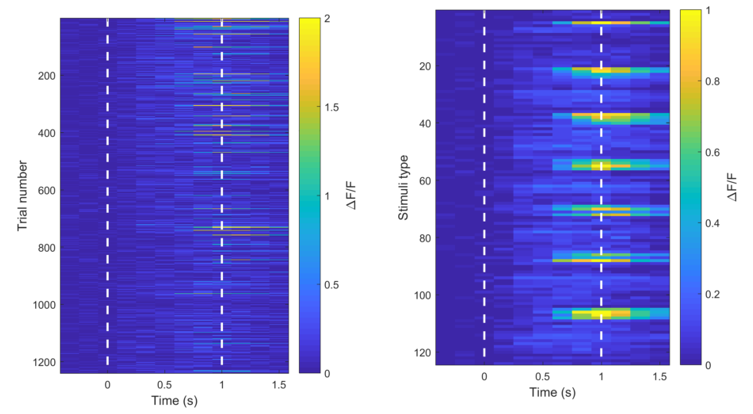
\includegraphics[width=14cm,height=14cm,keepaspectratio]{Figures/7.Results/individualSM/roi_29_mf379_pos5/roi29.png} 
\caption{SM protocol responses (dF/F) over time (s), for the example DS cell. Responses were baseline subtracted (0.5s) and stimulus onset centred at 0 s.
\newline \textbf{Left:} 1240 trial responses (10 repetitions, 124 trial types) as chronologically presented to the subjects, over the trial length. No structure is apparent.
\newline \textbf{Right:} Averaged repetition responses per trial type, ordered as determined on the text subsection \ref{DSexamplecell} over the trial length. Consistent structure is visible.}
\label{individualDStrials}
\end{figure}

Then we assess trial type responses within a given organization: First we show C stimuli responses, then S1 stimuli responses, and finally move to S1+C response profiles. We leave S2+C and S2 analysis for the population analysis section, focusing here on validating this protocol's analysis and interpreting the more simple found results in individual example cells.

In figure \ref{DSexamplecellcenter}, we observe that this cell portrays a large response to up center stimulation, but the responses for other directions are not substancial. This is a DS cell with up preferred direction. Figure \ref{DSexamplecellsurrounds} shows that surround-only stimulation did not hold any significant response for this cell, as required for this SM study.

\begin{figure}[H] \centering 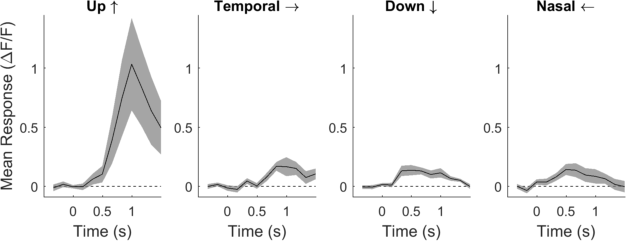
\includegraphics[width=11cm,height=11cm,keepaspectratio]{Figures/7.Results/individualSM/roi_29_mf379_pos5/1.png} 
\caption{Mean repetition trial response profiles for C conditions in the DS example cell, over trial time. The responses were baseline subtracted and the stimulus onset was centred at 0 s. Only the up center gratings direction evoked substantial significant responses.}
\label{DSexamplecellcenter}
\end{figure}

\begin{figure}[H] \centering 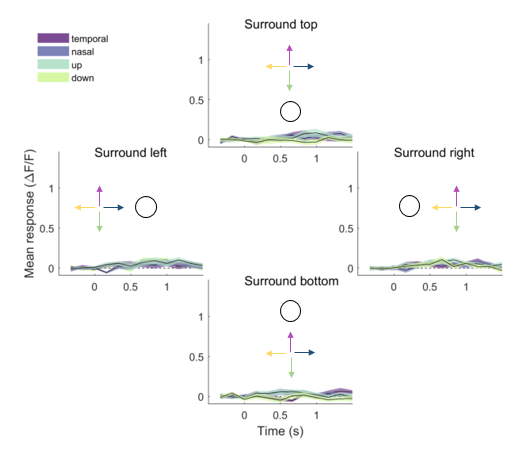
\includegraphics[width=10cm,height=10cm,keepaspectratio]{Figures/7.Results/individualSM/roi_29_mf379_pos5/2.png} 
\caption{Mean repetition trial response profiles for S1 conditions in the DS example cell, over trial time. The responses were baseline subtracted and the onset was at 0 s. No significant responses were present for this surround-only condition, as intended for SM analysis.
\label{DSexamplecellsurrounds}}
\end{figure}

In figure \ref{DSexamplecellSM} some SM results are shown. Only when center grating stimulation was on the up direction did any significant response hold (for simplicity not shown here, no responses were present either for horizontally or vertically positioned surrounds with non up-oriented center stimuli, supplementary figure \ref{s1}).

In this case, only surround suppression was present. Qualitatively, highest suppression is manifested for when surround stimulation is on the right, going in the down direction, followed by when it is also on the right, but going in the up direction and when it is going nasally in the top position.

\begin{figure}[H] \centering 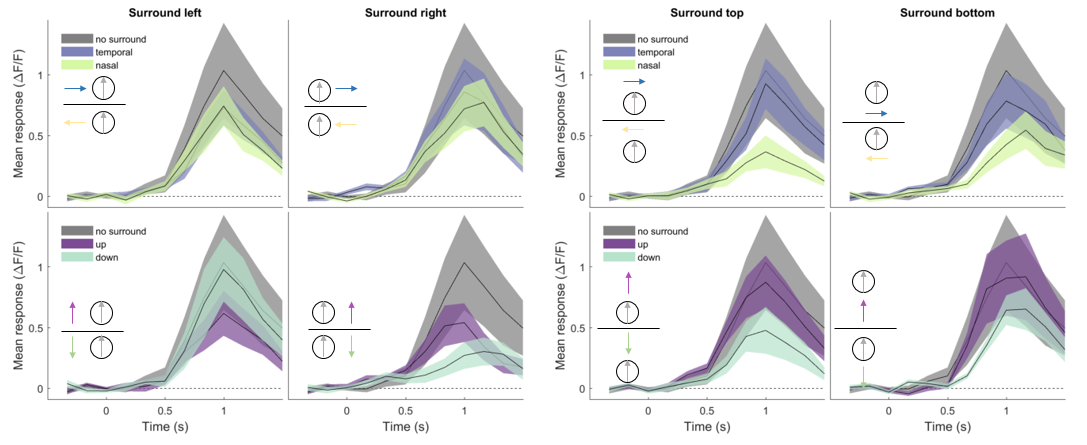
\includegraphics[width=15.9cm,height=15.9cm,keepaspectratio]{Figures/7.Results/individualSM/roi_29_mf379_pos5/3.png} 
\caption{S1+C effects for each center direction condition, averaged over 10 repetitions, over trial time, for the DS example cell. The responses were baseline subtracted and the onset was at 0 s. For comparisons, responses for center-only condition are represented as gray curves in each plot.
S1L+C, S1R+C, S1T+C and S1B+C respectively at each column, for up center condition. For each, surround gratings can be going temporally (blue curve), nasally (yellow curve), up (purple curve) or down (green curve).}
%S1L+C and S1R+C responses for center going temporally (left module), down (middle module) or nasally (right module). S1T+C and S1B+C responses are not shown here, as they portray similar non-responsive profiles.}
\label{DSexamplecellSM}
\end{figure}

Averaging the S1+C conditions over all of the center directions we find small responses and slight suppression average results (figure \ref{DSexamplecellaverage}), as these were diluted by the very little responses of this cell for other than up-directions. Suppression effects show the same qualitative results as above, but these were smaller than for the non-averaged center-up conditions; Over the population, facilitatory effects were rare, so this preliminary analysis did suggest (as realized with more examples and population analysis) that further analysis should be confined to the responsive center conditions, for minimizing noise additions to the results.

\begin{figure}[H] \centering 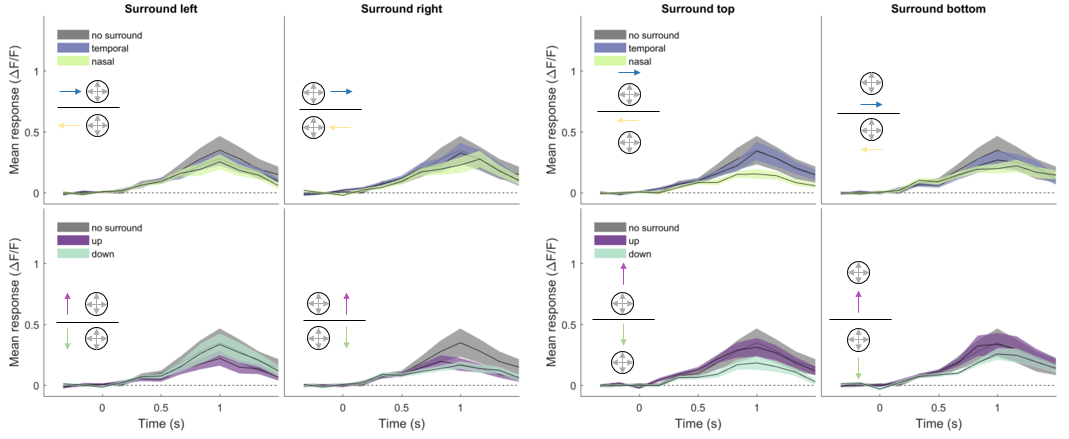
\includegraphics[width=15.9cm,height=15.9cm,keepaspectratio]{Figures/7.Results/individualSM/roi_29_mf379_pos5/4.png} 
\caption{Average responses for S1L+C, S1R+C, S1T+C and S1B+C, respectively from left to right. Conditions over all of the center directions.
\label{DSexamplecellaverage}}
\end{figure}

\subsection{OS example cell}

We present now the same sort of analysis for an OS example cell.

Again, in figure \ref{individualOStrials}, we see that plotting responses ordered chronologically does not show a response structure, but when these spikes are organized by stimulus type, here in the same number as explained in the above subsection, evident structure appears.

\begin{figure}[H] \centering 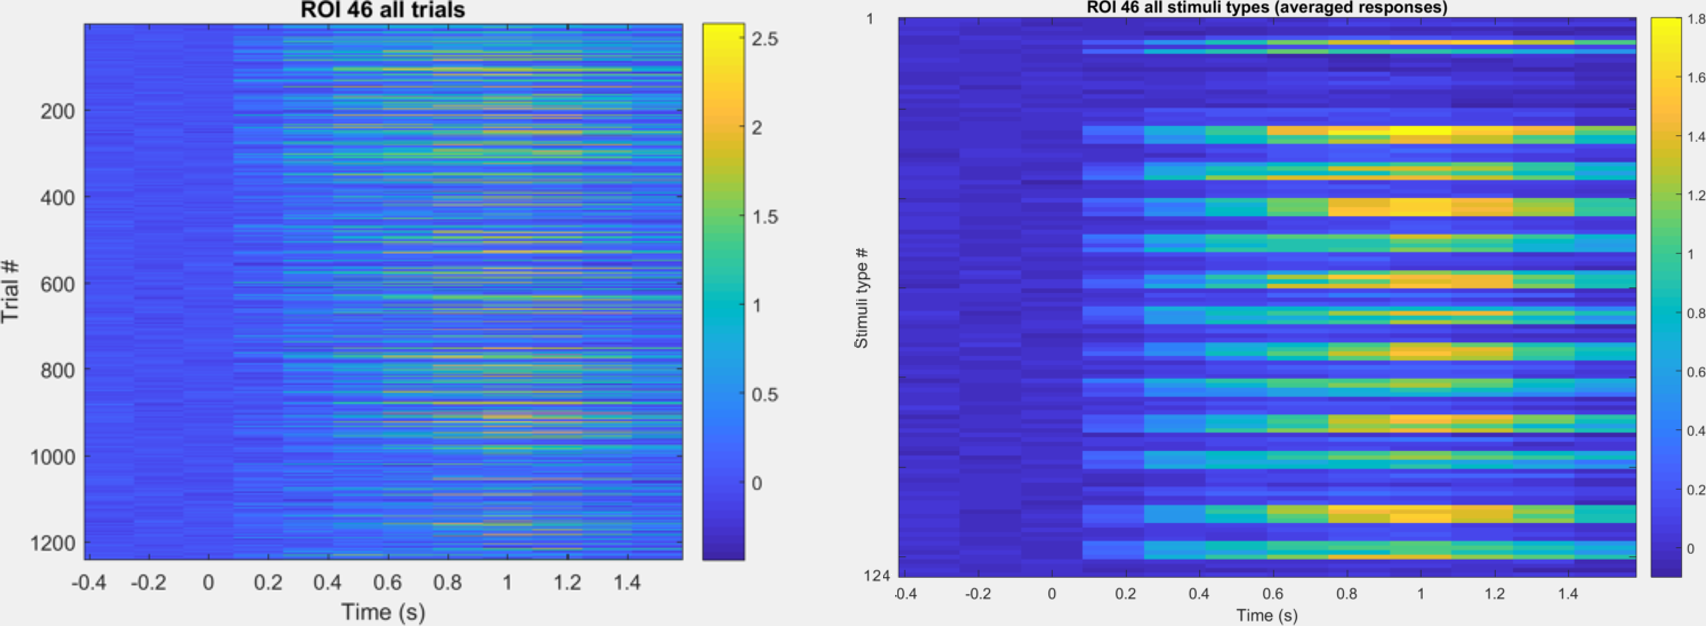
\includegraphics[width=14cm,height=14cm,keepaspectratio]{Figures/7.Results/individualSM/roi_46_mf379_pos2/roi46.png} 
\caption{SM protocol responses (dF/F) over time (s), for the example OS cell. The responses were baseline subtracted (0.5 s) and the stimulus onset was at 0 s.
\newline \textbf{Left:} 1240 trial responses (10 repetitions, 124 trial types) as chronologically presented to the subjects, over the trial length. No structure is apparent.
\newline \textbf{Right:} Averaged repetition responses per trial type, ordered as determined on the text subsection \ref{DSexamplecell} over the trial length. Consistent structure is visible. \label{individualOStrials}}
\end{figure}

We follow with the center only stimulation responses over the trial length (figure \ref{OSexamplecellcenter}). The cell is noticeably OS, with horizontal preferred orientation. As with the previous cell, no S1 condition held significant non-null responses, as intended for these SM analysis.

\begin{figure}[H] \centering 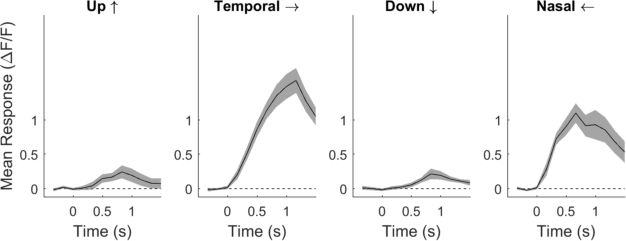
\includegraphics[width=11cm,height=11cm,keepaspectratio]{Figures/7.Results/individualSM/roi_46_mf379_pos2/1.png} 
\caption{Mean repetition trial response profiles for C conditions in the OS example cell, over trial time. The responses were baseline subtracted and the stimulus onset was centred at 0 s. The temporal and nasal center gratings directions evoked substantial significant responses, deeming the horizontal orientation the preferred orientation of this OS cell.}
\label{OSexamplecellcenter}
\end{figure}

In regards to the SM results, figure \ref{OSexamplecellSM} shows the most relevant profiles for this cell - for center going temporally or nasally. Other center direction conditions held no significant substantial  responses. 

In this case, the cell was barely suppressed by the surround, with the most noticeable effect being a facilitation one, for the center gratings going nasally, surround on top conditions, with surround going either nasally or temporally. As will be shown in the next section, these facilitatory effects were rare across the analysed population.

\begin{figure}[H] \centering 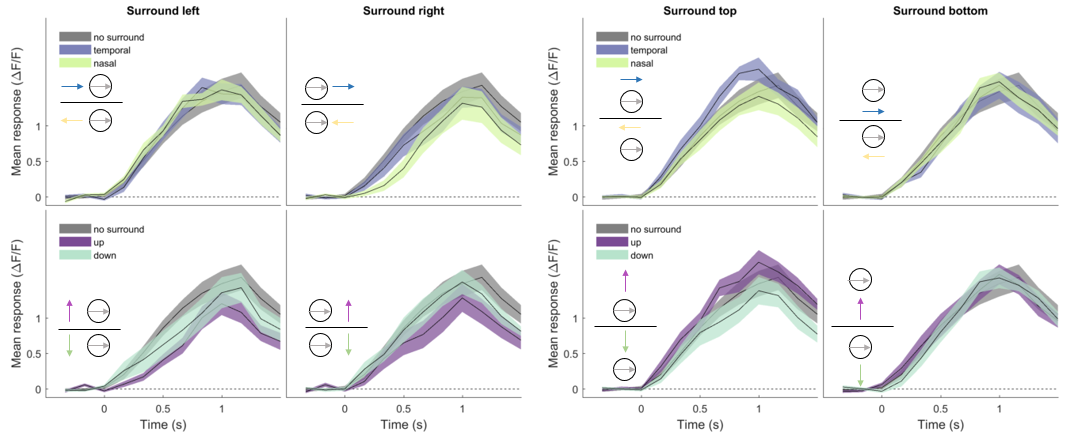
\includegraphics[width=15.9cm,height=15.9cm,keepaspectratio]{Figures/7.Results/individualSM/roi_46_mf379_pos2/3.png} 
\caption{S1+C effects for each center direction condition, averaged over 10 repetitions, over trial time, for the OS example cell. The responses were baseline subtracted and the onset was at 0 s. For comparisons, responses for center-only condition are represented as gray curves in each plot.
S1L+C, S1R+C, S1T+C and S1B+C respectively at each column, for temporal center condition. For each, surround gratings can be going temporally (blue curve), nasally (yellow curve), up (purple curve) or down (green curve).}
\label{OSexamplecellSM}
\end{figure}

\begin{figure}[H] \centering 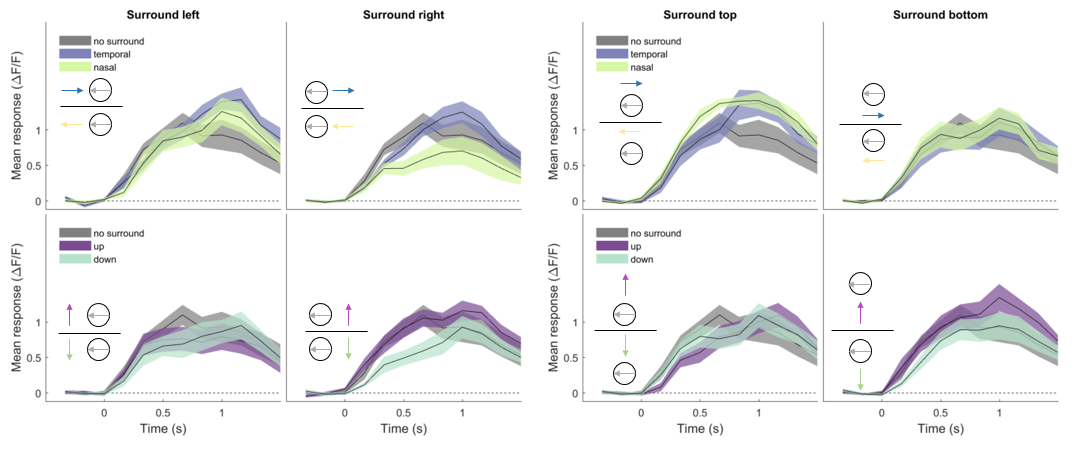
\includegraphics[width=15.9cm,height=15.9cm,keepaspectratio]{Figures/7.Results/individualSM/roi_46_mf379_pos2/4.png} 
\caption{S1+C effects for each center direction condition, averaged over 10 repetitions, over trial time, for the OS example cell. The responses were baseline subtracted and the onset was at 0 s. For comparisons, responses for center-only condition are represented as gray curves in each plot.
S1L+C, S1R+C, S1T+C and S1B+C respectively at each column, for nasal center condition. For each, surround gratings can be going temporally (blue curve), nasally (yellow curve), up (purple curve) or down (green curve).}
\label{OSexamplecellSM}
\end{figure}

\section{SM analysis - cells population}

After last section's scattered analysis, we follow with more general, systematic analysis, by investigating average effects on all of the cells population.

\subsection{Data ROI groups}

Firstly, we divide the available ROIs into different group classes.

In total, 2728 cells' trace responses were extracted from Suit2p pipeline (see section \ref{sec:Suit2ppipeline}).  From these, 2869 cells were responsive to some visual stimulation, as assessed with sign-tests over the differences between responses for stimulation and baseline times ($p<0.05$), for any of the trial types. Within these, 897 cells were significantly responsive to at least one of the center-only conditions (assessed with the same statistical test). This was the first condition for the cell to be SM analysed. These values are showed to scale on figure \ref{groups1}.

%\begin{figure}[H] \centering \includegraphics[width=5cm,height=5cm,keepaspectratio]{Figures/7.Results/data/ROIvisualCenter.png} 
%\caption{Scaled depiction of cell numbers for each responsiveness group condition: ROIs selected by Suit2p pipeline (blue), visually responsive ROIs (red) and center-only condition(s) responsive ROIs (green).}
%\label{groups1}
%\end{figure}

Within this last group of center-responsive ROIs, cells could also be divided in OS cells (n=472) and DS cells (n=371). Some DS cells were also OS cells (n=243). The remaining 600 cells were not found orientation selective. These assessments were made as described in subsection \ref{subsec:tuningresults}, but using the data set from the SM protocol's center only conditions. A scaled cell numbers diagram is presented in figure \ref{groups2}.
OS and DS cells were separately analysed in some relevant comparison cases in section \ref{sec:comparisons}.
%
%\begin{figure}[H] \centering 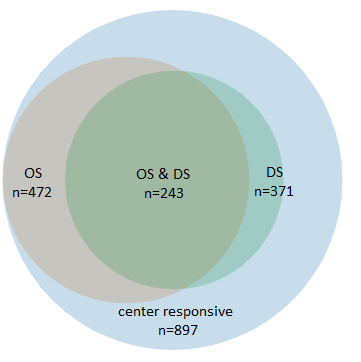
\includegraphics[width=5cm,height=5cm,keepaspectratio]{Figures/7.Results/data/centerOSDS.png} 
%\caption{Scaled depiction of cell numbers for each selectivity condition:Center responsive cells (blue), OS cells (red) and DS cells (green).}
%\label{groups2}
%\end{figure}

\begin{figure}[h]
    \centering
    \begin{minipage}[t]{.4\textwidth}
        \centering
\includegraphics[width=6cm,height=6cm,keepaspectratio]{Figures/7.Results/data/ROIvisualCenter.png} 
\caption{Scaled depiction of cell numbers for each responsiveness group condition: ROIs selected by Suit2p pipeline (blue), visually responsive ROIs (red) and center-only condition(s) responsive ROIs (green).\label{groups1}}
\end{minipage}\hspace{1cm}
\begin{minipage}[t]{0.4\textwidth}
\centering
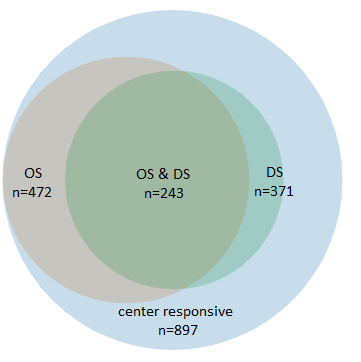
\includegraphics[width=6cm,height=6cm,keepaspectratio]{Figures/7.Results/data/centerOSDS.png} 
\caption{Scaled depiction of cell numbers for each selectivity condition: Center responsive cells (blue), OS cells (red) and DS cells (green).\label{groups2}}
\end{minipage}
\end{figure}

For all of the SM analysis, cells ought to be responsive to at least one of the center conditions, but were also conservatively required to hold no significant response for any of the relevant surround only conditions. In this way, we could be sure that independently of the receptive field measurements of each cell, the portrayed effects were in fact surround modulatory effects.
The majority (n=788) of the center responsive cells did not respond to any of the surrounds, showing that for these sessions the stimuli responses were well centred. For some of the analysis, we were able to loosen the requirements: There were 812 cells responding to the center and not to the horizontally positioned surrounds, while 864 cells responded to the center and not to the vertically positioned surrounds. These groups were again assessed with the same statistical sign-tests. These groups were used when analysis was projected in only one of the surround's position axis. Figure \ref{groups3} shows a cell numbers diagram for each of these conditions on the left, and the same simplified but scaled diagram on the right.

\begin{figure}[H] \centering 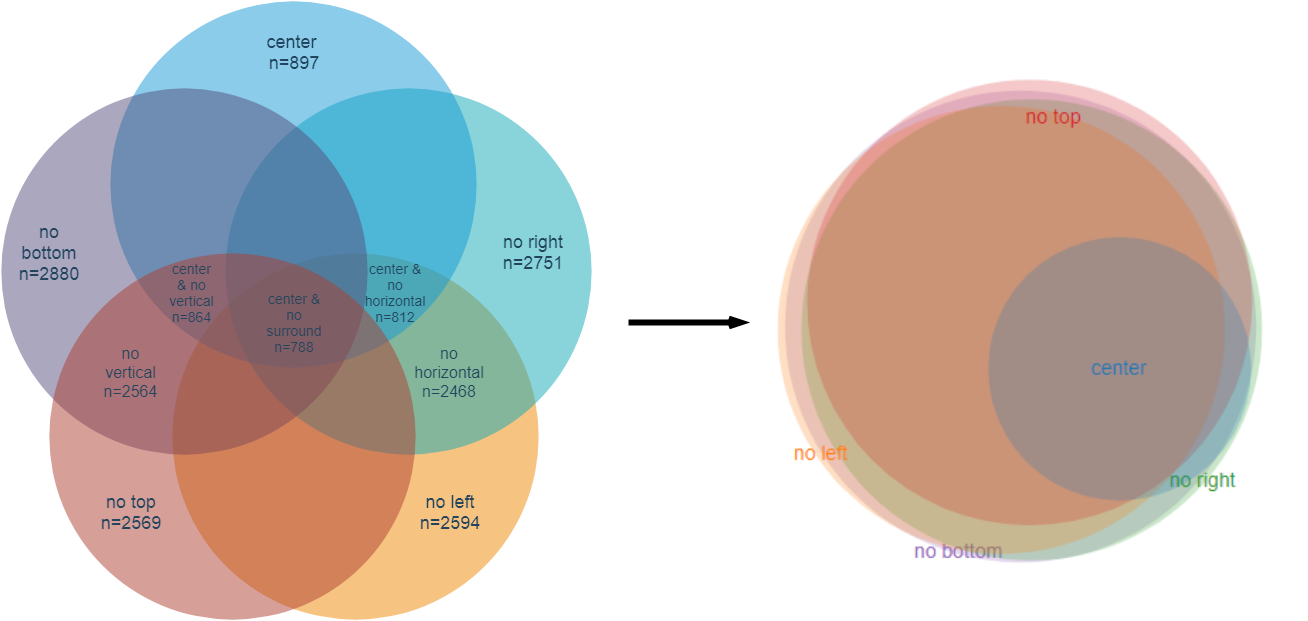
\includegraphics[width=15cm,height=15cm,keepaspectratio]{Figures/7.Results/data/SMdata.png} 
\caption{Diagram of cell numbers for each center and surround responsiveness condition, with detailed most relevant values (left) and scaled (right): Center responsive cells (blue), no S1L stimuli conditions responsive cells (yellow), no S1R stimuli conditions responsive cells (green), no S1T stimuli conditions responsive cells (red) and no S1B stimuli conditions responsive cells (green).}
\label{groups3}
\end{figure}

\subsection{RF center positions and SM protocol center-only: all population and per animal}

Beginning the following analysis, we first noticed that the dataset ROIS tended to become very weakly responsive for the second half of the SM protocol, possibly due to its extended length and anaesthesia condition. For this reason, all of the following analysis was done regarding only the 10 first trials of the SM protocol, for each trial type (1240 total stimuli). 


Starting with the population analysis, we first investigated the overall RF center locations of all the extracted ROIs, specifying also for the selected ROIs (center responsive and not surround only responsive). We found a consistent bias in our data set for ROIs with higher elevation RF centres, for both the cases of all of the ROIs and the case of the selected ROIs (\ref{allRF}).  The same bias was found when separating the ROIs per animal and per session (for an example, \ref{exRF}). For this reason, subsequent analysis was not conducted for comparing top and bottom conditions, nor for comparing horizontally-positioned with vertically-positioned surround conditions.

\begin{figure}[h]
    \centering
    \begin{minipage}[t]{.4\textwidth}
        \centering 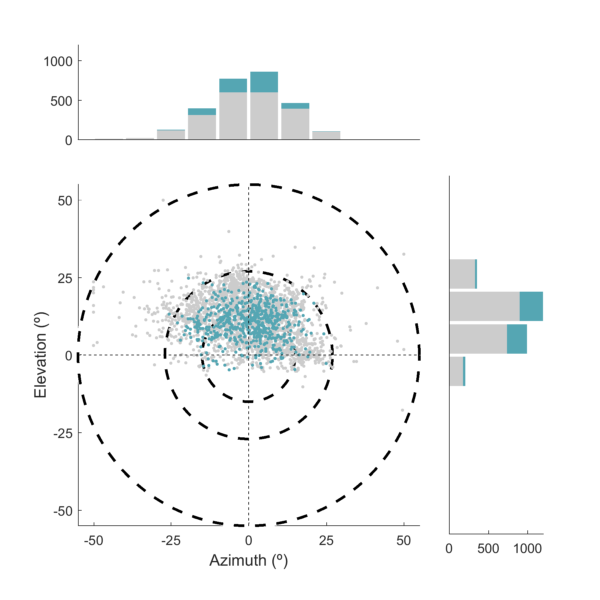
\includegraphics[width=7.8cm,height=7.8cm,keepaspectratio]{Figures/7.Results/finalPopulation/sel/popPlots_rfPositions_allSessions.png} 
\caption{RF center coordinates for all the ROIs (gray, n=3728), specifying the selected center responsive and not surround only responsive ROIs (turquoise, n=788). Dashed lines represent the stimuli sizes: inner circle for the center stimuli, outer annulus for the different surround positions. Frequency histograms for both elevation (side) and azimuth (top) locations.}
\label{allRF}
\end{minipage}\hspace{1cm}
\begin{minipage}[t]{.4\textwidth}
\centering 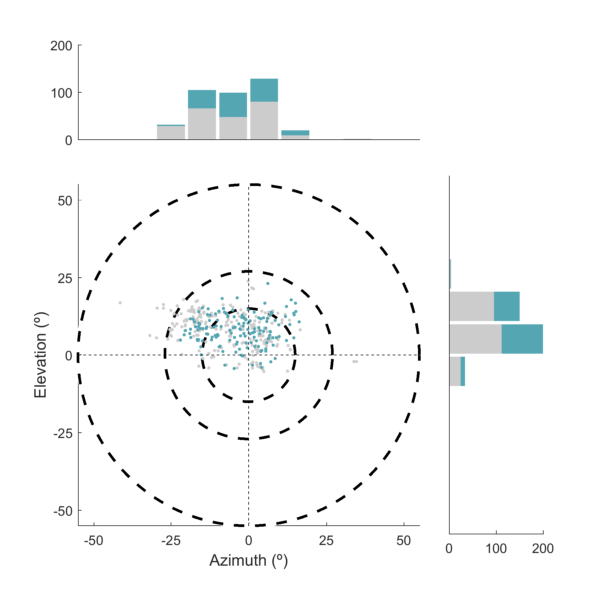
\includegraphics[width=7.8cm,height=7.8cm,keepaspectratio]{Figures/7.Results/finalPopulation/sel/popPlots_RFpos_Animal4_Session5.png} 
\caption{RF center coordinates for the ROIs from an example animal and session (gray, n=236), specifying the selected center responsive and not surround only responsive ROIs (turquoise, n=153).} 
\label{exRF}
\end{minipage}
\end{figure}
%\begin{figure}[H] \centering 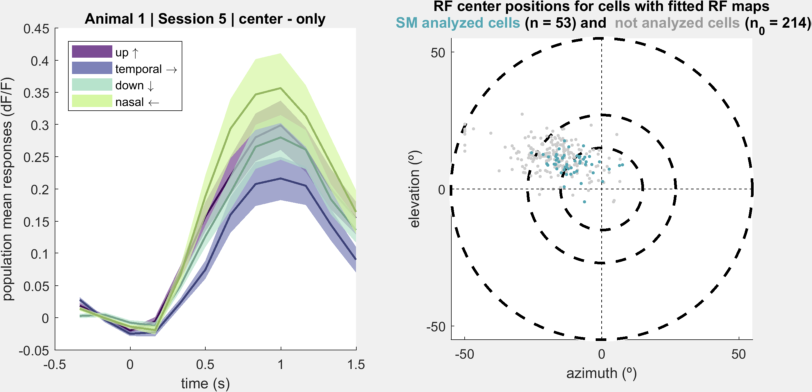
\includegraphics[width=12cm,height=12cm,keepaspectratio]{Figures/7.Results/population/sel/2_popPlots_Animal1_Session5.png} 
%%\caption{2 popPlots Animal1 Session5.} 
%\end{figure}

%\begin{figure}[H] \centering 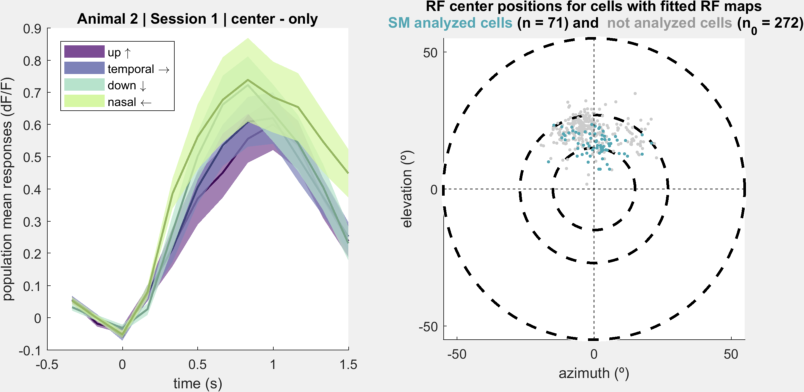
\includegraphics[width=12cm,height=12cm,keepaspectratio]{Figures/7.Results/population/sel/3_popPlots_Animal2_Session1.png} 
%%\caption{3 popPlots Animal2 Session1.} 
%\end{figure}
%
%\begin{figure}[H] \centering 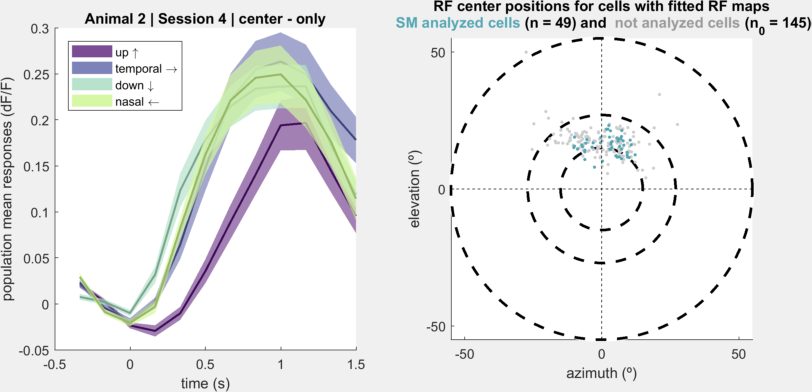
\includegraphics[width=13cm,height=13cm,keepaspectratio]{Figures/7.Results/population/sel/4_popPlots_Animal2_Session4.png} 
%%\caption{4 popPlots Animal2 Session4} 
%\end{figure}
%
%\begin{figure}[H] \centering \includegraphics[width=13cm,height=13cm,keepaspectratio]{Figures/7.Results/population/sel/5_popPlots_Animal2_Session5.png} 
%%\caption{5_popPlots_Animal2_Session5} 
%\end{figure}



%\begin{figure}[H] \centering \includegraphics[width=13cm,height=13cm,keepaspectratio]{Figures/7.Results/population/sel/7_popPlots_Animal3_Session1.png} 
%%\caption{7_popPlots_Animal3_Session1} 
%\end{figure}
%
%\begin{figure}[H] \centering \includegraphics[width=13cm,height=13cm,keepaspectratio]{Figures/7.Results/population/sel/8_popPlots_Animal4_Session2.png} 
%%\caption{8_popPlots_Animal4_Session2} 
%\end{figure}
%
%\begin{figure}[H] \centering \includegraphics[width=13cm,height=13cm,keepaspectratio]{Figures/7.Results/population/sel/9_popPlots_Animal4_Session5.png} 
%%\caption{9_popPlots_Animal4_Session5} 
%\end{figure}

Next, we assess the selected ROIs responses to the center only conditions (for the four cardinal directions). For this, we separate the cell's by their orientation selectivity. Non-OS cells have distributed responses across the four directions (figure \ref{nonOS}). We are also able to observe that different neurons respond at different times, in relation to the stimulus onset.

\begin{figure}[H] \centering \includegraphics[width=12cm,height=12cm,keepaspectratio]{Figures/7.Results/finalPopulation/sel/popPlots_nonOS_centerOnly.png} 
\caption{Normalized responses across non-OS neurons, for the C conditions, each panel respectively for on of the four directions up, temporal, down and nasal. Responses are computed as the mean of the trial repetitions (10) for that cell and that stimulus condition. Dashed lines mark stimulus onset and offset.} 
\label{nonOS}
\end{figure}

We then do the same verifications, for OS selected cells: OS neurons with horizontal preferred orientation and  OS (figure \ref{OShorz}) neurons with vertical preferred orientation (figure \ref{OSvert}). Indeed, we find that horizontal OS cells respond more for temporal and nasal moving center gratings, while vertical OS cells respond for up and down moving center gratings.
\vspace*{-0.4cm}
\begin{figure}[H] \centering \includegraphics[width=11cm,height=11cm,keepaspectratio]{Figures/7.Results/finalPopulation/sel/popPlots_horzOS_centerOnly.png} 
\vspace*{-0.2cm}\caption{Normalized responses across horizontal OS neurons, for the C conditions, each panel respectively for one of the four directions up, temporal, down and nasal. Responses are computed as the mean of the trial repetitions (10) for that cell and that stimulus condition. Dashed lines mark stimulus onset and offset.} \label{OShorz}
\end{figure}
\vspace*{-0.4cm}
\begin{figure}[H] \centering \includegraphics[width=11cm,height=11cm,keepaspectratio]{Figures/7.Results/finalPopulation/sel/popPlots_vertOS_centerOnly.png} 
\vspace*{-0.2cm}\caption{Normalized responses across vertical OS neurons, for the C conditions, each panel respectively for one of the four directions up, temporal, down and nasal. Responses are computed as the mean of the trial repetitions (10) for that cell and that stimulus condition. Dashed lines mark stimulus onset and offset.} \label{OSvert}
\end{figure}

\subsection{Comparisons between conditions}
\label{sec:comparisons}

At this point, the analysis continues with comparisons between multiple S1+C and S2+C surround and center configurations, to investigate the existence of biases or trends regarding the surround positions, orientations, directions, center orientation, direction, OS and/or DS preferences, as well as combinations of these factors. Each comparison was thus done with different numbers of cells and different stimuli numbers of conditions. 

For each of these comparisons, the intended outputs are both the effect's strength and statistical significance. 

\begin{enumerate}
\item First, we regard how differently does the population respond to the center-only C condition and the first of the pooled configuration sets to compare, within a scatter-plot (top, first panel of image \ref{1}). 

\item Second, we regard the same for the other pooled configuration set to compare (top, second of image \ref{1}). 

\item The population averaged (across ROIs, pooled conditions and trial repetitions) response trace is also extracted for each of these configuration sets and compared with the population averaged (across ROIs and trial repetitions) appropriate center-only condition response trace (top third panel of image \ref{1}, first panel of all subsequent comparison figures).

\item Next, we compare the responses between the two configuration sets, within a scatter plot (bottom first panel of image \ref{1}).

\item Then, we compare the SM indexes ($SMI$) of the pooled ROIs - a measurement of the surround modulatory effect strenght-, in a scatter-plot, for each configuration set (bottom, second panel of image \ref{1}; second panel of the other comparison images). The average resulted is also marked with standard deviation error bars. For every stimuli surround-center condition, one can compute:

\begin{equation}
SMI_a=\dfrac{\bar{R_{a}}-\bar{R_C}}{\bar{R_a}+\bar{R_C}}
\end{equation}

With $\bar{R_a}$ the average (across trial repetitions and stimulus time) surround and center condition at hand, and $\bar{R_C}$ the average  (across trial repetitions and stimulus time) of the respective center-only condition.

The cell's $SMI$ to consider for a given set of configurations then averages across the $SMI_a$s for each of the pooled conditions.

A method to regard the effects tendencies and significance, involves single-neuron analysis: assessing how many neurons respond significantly to one or to the other set of configurations being compared, with a rank-sum test, at p-value threshold $p=0.05$. These are presented in the scatter-plot of each figure, respectively coloured, along with its counts. 

\item Finally, we plot the frequency histogram of the difference between the compared SM effects for one and the other configuration sets, within the population,$\Delta SMI$ (last panels of image \ref{1} and all following comparison figures). We additionally calculate the average of these $\Delta SMI$, $\mu$ and the correspondent p-value, calculated with a sign-test. This measures SM asymmetry between the two configuration sets and correspondent significance.

\end{enumerate}

At the side of each comparison figure, there's a diagram of the pooled stimuli conditions for each configuration set (blue and red). We enhance the frame for configuration sets towards which the computed $\mu$ tend to - that is, the configuration set for with the population tends to entail higher suppression, on average - when the obtained p-value is less than $0.05$. This expresses SM tendencies towards one or the other configuration set.

However, in a more statistically conservative approach, considering the multi-inference nature of this study, the Holm-Bonferroni method was used to compensate the multiple comparisons problem (see in the statistical tools chapter, \ref{sec:StatisticalTests}), delivering a powerful way of assessing each comparison's significance. The p-value family threshold was $\alpha=0.05$. If a test was accepted, with the Bonferroni correction, an asterisk is also drawn in the last panel of the respective comparison figure to express statistical significance.

\subsubsection{Surround number effect}

We start with the surround number effect: We find a large and significant differential effect of higher suppression for double surround conditions over one surround condition. Moreover, suppression was also notable, for all of the conditions, in particular for the 2S+C pooled conditions.

\begin{figure}[H] \centering \includegraphics[width=12cm,height=12cm,keepaspectratio]{Figures/7.Results/finalPopulation/sel/diagrams/1.png} 
\caption{Surround number effect: Single surround versus double surround, with center gratings moving in the most responsive direction; $n=788$, 16 (single) and 8 (double) pooled conditions per configuration set.} 
\end{figure}

Across comparisons, we consistently found that two surround conditions held the most differentiated effects. This was a noted result, and thus we next perform the comparisons, when possible, with the 2S+C stimuli sets.

We disregard the intermediate panels 1, 2 and 4 in the next comparison plots. 

\subsubsection{Surround-RF distance effect and Surround position effect}

%\begin{figure}[H] \centering \includegraphics[width=11cm,height=11cm,keepaspectratio]{Figures/7.Results/finalPopulation/sel/diagrams/2.png} 
%%\caption{13_popPlots_VisROIs_CprefDir_Snumber} 
%\end{figure}


%\begin{figure}[H] \centering \includegraphics[width=12cm,height=12cm,keepaspectratio]{Figures/7.Results/finalPopulation/sel/13_popPlots_VisROIs_CprefDir_Snumber.png} 
%%\caption{13_popPlots_VisROIs_CprefDir_Snumber} 
%\end{figure}
%
%\begin{figure}[H] \centering \includegraphics[width=12cm,height=12cm,keepaspectratio]{Figures/7.Results/finalPopulation/sel/14_popPlots_VisROIs_CprefDir_SposLeftRight.png} 
%%\caption{14_popPlots_VisROIs_CprefDir_SposLeftRight} 
%\end{figure}

Comparing the left versus right surround conditions, we first assessed the relationship between the SMI and the RF azimuth center position. We found, with a multiple regression, that, for both left and right cases, the SMI depended linearly on the azimuth RF center coordinate (p=0.002 and p=0.0056, respectively - figure \ref{reg}.

We then wanted to find if this effect differed between the left and the right surround cases. For this, we held a double permutation test with 10000 resamples, for both the slope and the offset of the regression for SMI_{Left} and for SMI_{Right}, and tested the null hypothesis that the new resamples, the same ROIs, but randomly attributed to either SMI_{Left} regression or SMI_{Right} regression, did not differ from the original distribution of ROI points. We obtained for the offset $p=0.1472$ and for the slope $p=0.8712$. This means that we cannot reject the null hypothesis, so the differences between left and right cases regression slopes and offsets are thus regarded as non significant. This finding suggests a distance effect: The SMI becomes increasingly stronger, the closer the RF center is to it, even though, we note again, the surround-only condition does not evoke any response. 

\begin{figure}[H] \centering \includegraphics[width=10cm,height=10cm,keepaspectratio]{Figures/7.Results/finalPopulation/sel/reg.png} 
\caption{SMI of the selected ROIs, across S1L+C conditions (left panel) and S1R+C conditions (right panel), as a function of azimuth RF center coordinate. Superimposed multiple regression line, equation and p-value.} \label{reg}
\end{figure}

Finding this distance effect, we then chose a balanced dataset across azimuth, and compared the left and right surround modulatory effects (figure \ref{2}). A tendency seemed to appear for left surround suppressing more than right surround, but this result held no significance.

\begin{figure}[H] \centering \includegraphics[width=12cm,height=12cm,keepaspectratio]{Figures/7.Results/finalPopulation/sel/diagrams/2.png} 
\caption{Position effect: left versus right surround, with center moving in the most responsive direction; Balanced dataset over RF azimuth location; $n=434$, 4 pooled conditions per configuration set.} \label{2}
\end{figure}

\subsubsection{Surround direction effect}

To determine the surround direction effect, we started by comparing the up versus down conditions (figure \ref{3}, double surround; Weaker qualitative result with the same tendency for one surround, as was the case in all following comparisons). We found no differential effect and high consistent suppression.

\begin{figure}[H] \centering \includegraphics[width=12cm,height=12cm,keepaspectratio]{Figures/7.Results/finalPopulation/sel/diagrams/3.png} 
\caption{Direction effect: up versus down surround, with center moving in the most responsive direction and double surround conditions;  $n=788$, 2 pooled conditions per configuration set.}
\label{3} 
\end{figure}

For temporal versus nasal conditions (figure \ref{4}), the differential effect tended to increase, with higher suppression for nasally moving stimuli. However, correcting for multiple inferences, the result was not found significant.

\begin{figure}[H] \centering \includegraphics[width=12cm,height=12cm,keepaspectratio]{Figures/7.Results/finalPopulation/sel/diagrams/4.png} 
\caption{Direction effect: temporal versus nasal surround, with center moving in the most responsive direction and double surround conditions;  $n=788$, 2 pooled conditions per configuration set.} 
\label{4}
\end{figure}

\subsubsection{Surround orientation effect}

We follow with the orientation effect (figure \ref{5} A tendency appeared for higher suppression when surround stimuli moving horizontally versus moving vertically. However, corrected with Bonferroni method, this result did not hold significant.

\begin{figure}[H] \centering \includegraphics[width=12cm,height=12cm,keepaspectratio]{Figures/7.Results/finalPopulation/sel/diagrams/5.png} 
\caption{Orientation effect: horizontal versus vertical surround, with center moving in the most responsive direction and double surround conditions;  $n=788$, 4 pooled conditions per configuration set.} 
\label{5}
\end{figure}

\subsubsection{Surround orientation alignment effect (position and orientation)}

Combining position and orientation surround effects, we regard the surround orientation alignment effect of stimuli in the colinear versus the flanking alignments (figure \ref{6}). We found a substantial and significant difference between the pooled configuration sets: colinearity suppressed to a significantly higher degree than flanking conditions.

\begin{figure}[H] \centering \includegraphics[width=12cm,height=12cm,keepaspectratio]{Figures/7.Results/finalPopulation/sel/diagrams/6.png} 
\caption{Alignment effect: colinear versus flanking surround, with center moving in the most responsive direction and double surround conditions;  $n=788$, 4 pooled conditions per configuration set.} 
\label{6}
\end{figure}

\subsubsection{Center and surround relative orientation effect, with center OS preference}

Now regarding as well the center gratings orientation of movement, relative to the surrounds, we assess the center-surround (C-S) relative orientation effect (figure \ref{7}). A significant large result is observed: Iso-oriented surround suppresses tendentiously more than cross-oriented surround gratings.

\begin{figure}[H] \centering \includegraphics[width=12cm,height=12cm,keepaspectratio]{Figures/7.Results/finalPopulation/sel/diagrams/7.png} 
\caption{Relative orientation effect: iso-oriented versus cross-oriented surround, with center moving in the most responsive direction and double surround conditions;  $n=788$, 8 pooled conditions per configuration set.} 
\label{7}
\end{figure}

We also check this comparison for OS only cells, first when the center is in the preferred orientation (image \ref{8}). The same qualitative result holds significant, however less strong than in the non-OS case.

\begin{figure}[H] \centering \includegraphics[width=12cm,height=12cm,keepaspectratio]{Figures/7.Results/finalPopulation/sel/diagrams/8.png} 
\caption{Relative orientation effect: iso-oriented versus cross-oriented surround, OS ROIs with center in the preferred orientation and double surround conditions;  $n=472$, 8 pooled conditions per configuration set.} \label{8}
\end{figure}

The same comparison is then performed for OS only cells, when the center is in the anti-preferred orientation (image \ref{9}). The same tendency as in the previous cases is apparent, but significance is lost. In fact, this condition has much fewer available ROIs ($n=68$) since for this analysis the neurons must be OS for one orientation, but still respond to the other to be chosen, which is more stringent than for previous ROI sets.

\begin{figure}[H] \centering \includegraphics[width=12cm,height=12cm,keepaspectratio]{Figures/7.Results/finalPopulation/sel/diagrams/9.png} 
\caption{Relative orientation effect: iso-oriented versus cross-oriented surround, OS ROIs with center in the anti-preferred orientation and double surround conditions;  $n=68$, 8 pooled conditions per configuration set.} \label{9} 
\end{figure}

\subsubsection{Interactions between surround orientation alignment and surround-center relative orientation effects}

We now pool different conditions within the orientation alignment and the relative orientation effects, to investigate interaction effects between these two factors.

First, we take the collinear versus flanking effects, for iso-oriented stimuli (figure \ref{10}). We obtain a large significant average $\Delta SMI$ result, for higher colinear suppression.

\begin{figure}[H] \centering \includegraphics[width=12cm,height=12cm,keepaspectratio]{Figures/7.Results/finalPopulation/sel/diagrams/10.png} 
\caption{Orientation alignment effect, for iso-oriented center-surround: colinear versus flanking surround, with center moving in the most responsive direction and double surround conditions;  $n=788$, 4 pooled conditions per configuration set.} \label{10} 
\end{figure}

Then, we regard the collinear versus flanking effects, for cross-oriented stimuli (figure \ref{11}). A substantial differential trend is portrayed, again in favour of higher collinear suppression. However, when Bonferroni-correcting, the effect does no amount to be significant.

\begin{figure}[H] \centering \includegraphics[width=12cm,height=12cm,keepaspectratio]{Figures/7.Results/finalPopulation/sel/diagrams/11.png} 
\caption{Orientation alignment effect, for cross-oriented center-surround: colinear versus flanking surround, with center moving in the most responsive direction and double surround conditions;  $n=788$, 4 pooled conditions per configuration set.} \label{11} 
\end{figure}

In this way, we regard the SMIs of the four configuration sets jointly \ref{anova1} as four \textit{groups}: iso-oriented and collinear, iso-oriented and flanking, cross-oriented and collinear, cross-oriented and flanking.

\begin{figure}[H] \centering \includegraphics[width=10cm,height=10cm,keepaspectratio]{Figures/7.Results/finalPopulation/sel/popPlots_VisROIs_Cor_2SalignmentAngle.png} 
\caption{Orientation alignment and center-surround relative orientations effects. SMI per combined condition, for the same configuration sets as in figures \ref{10} and \ref{11}. Error bars correspond to the standard deviations.} 
\label{anova1}
\end{figure}

A two-way ANOVA was performed to assess how much of the data's $SMI$ variance each factor explained, as well as the interaction effect between the two of those factors. The results are in table \ref{tab:anova1}: 

Here, for each source row, the mean square $MS=\dfrac{\sum_{i=1}^n(y_i-\bar{y})^2}{dof}$ is first indicated, with n the number of ROIs, $y_i$ the SMI of the ith ROI, $\bar{y}$ the mean of the $n$ ROIs and dof the degrees of freedom associated with the source (1 for each factor, 3148 for the error); 

The second row presents the value of the $F$ statistic used to assess if there is a relationship between the means and the factor, given by the ratio between the source's mean squares ($MS_s$) and the error mean squares ($MS_e$); 

Finally, the third shows the p-value for factors and for interaction of factors, given by the probability of the F-test being larger than that value $F=\dfrac{MS_s}{MS_e}$. For a given source or interaction, a sufficiently small p-value indicates that that source significantly affects the mean values of $SMI$. 

We find that both the alignment, the angle and the interactive factor affect the distribution significantly. From the $F$ values, we find that the larger contribution comes from the orientation alignment effect, followed by the relative orientation and then by the interactive term.

\begin{table}[H]
\begin{center}\par
\scalebox{0.85}{
\begin{tabular}{c|cccccccccccccccccccccccccc}
\hline 
 
    
\multicolumn{1}{c}{Source of variability} & MS & F & p-value\\
           
           \hline
           \hline

\multicolumn{1}{c}{Orientation alignment} &2.6861 & 36.73 & 0 \\
\multicolumn{1}{c}{C-S relative orientation} &1.5627& 21.37 & 0\\
\multicolumn{1}{c}{Or alignment and C-S relative Or} & 0.4121 & 5.64 & 0.0177 \\
\multicolumn{1}{c}{Error}  0.07313\\
\hline
        
\end{tabular}}
 \caption{Two-way ANOVA results for the collinear versus flanking surround effect and iso-oriented versus cross-oriented C-S effect, and interactions.}
    \vspace{-5mm}
    \label{table1}
\end{center}
\end{table}

\subsubsection{Interactions between surround orientation alignment, surround-center relative orientation effects and center OS preference}

Keeping with the orientation alignment and center-surround relative orientation effects, we now focus also on the influence of the orientation selectivity of the ROI.

First, we assess the collinear versus flanking effects, for iso-oriented center-surround, for OS cells only, with the center gratings moving in the preferred orientation of the neuron (figure \ref{12}). We obtain a large, significant result of collinear surround stimuli suppressing more than flanking conditions.

\begin{figure}[H] \centering \includegraphics[width=12cm,height=12cm,keepaspectratio]{Figures/7.Results/finalPopulation/sel/diagrams/12.png} 
\caption{Orientation alignment effect, for iso-oriented center-surround: collinear versus flanking surround, OS ROIs with center in the preferred orientation and double surround conditions;  $n=472$, 4 pooled conditions per configuration set.} \label{12} 
\end{figure}

Then we investigate the collinear versus flanking effects, for cross-oriented center-surround, for OS cells only, with the center gratings moving in the preferred orientation of the neuron as well (figure \ref{13}). The differential effect shows a large trend for suppressing more collinear than flanking, but when corrected for multivariate analysis, the correspondent p-value did not hold significance.

\begin{figure}[H] \centering \includegraphics[width=12cm,height=12cm,keepaspectratio]{Figures/7.Results/finalPopulation/sel/diagrams/13.png} 
\caption{Orientation alignment effect, for cross-oriented center-surround: collinear versus flanking surround, OS ROIs with center in the preferred orientation and double surround conditions;  $n=472$, 4 pooled conditions per configuration set.} \label{13} 
\end{figure}

Then, we first compare the collinear versus flanking conditions, for iso-oriented center-surround, but following now with the anti-preferred direction of movement in the center (\ref{14}). No significant effect is observed.

\begin{figure}[H] \centering \includegraphics[width=12cm,height=12cm,keepaspectratio]{Figures/7.Results/finalPopulation/sel/diagrams/14.png} 
\caption{Orientation alignment effect, for cross-oriented center-surround: collinear versus flanking surround, OS ROIs with center in the anti-preferred orientation and double surround conditions;  $n=68$, 4 pooled conditions per configuration set.} \label{14}  
\end{figure}

Finally, we compare the collinear versus flanking conditions, for cross-oriented center-surround, with the anti-preferred direction of movement in the center (\ref{15}). Again, no significant average $\Delta SMI$ effect is observed for these conditions.

\begin{figure}[H] \centering \includegraphics[width=12cm,height=12cm,keepaspectratio]{Figures/7.Results/finalPopulation/sel/diagrams/15.png} 
\caption{Orientation alignment effect, for cross-oriented center-surround: collinear versus flanking surround, OS ROIs with center in the anti-preferred orientation and double surround conditions;  $n=68$, 4 pooled conditions per configuration set.} \label{15}
\end{figure}

With these results, we compare the SMIs of the eight configuration sets as eight groups, with all the refered combinations of colinear or flanking surrounds, iso-oriented or cross-oriented surrounds, and center in the preferred orientation or in the anti-preferred orientation (figure \ref{anova2}).

\begin{figure}[H] \centering \includegraphics[width=12cm,height=12cm,keepaspectratio]{Figures/7.Results/finalPopulation/sel/popPlots_VisROIs_COS_2SalignmentAngle.png} 
\caption{Orientation alignment, center-surround relative orientations and center stimulus orientation (in relation to OS preference) effects. SMI per combined condition, for the same configuration sets as in figures \ref{12} to \ref{15}. Error bars correspond to the standard deviations.} \label{anova2}
\end{figure}

Having assessed these factor combination comparisons, we now use a 3-way ANOVA to investigate the influence of the orientation alignment, relative orientation and orientation selectivity, as well of the possible interaction effects. The results are summarized in table \ref{table2}. The effect of the stimulus in the center (relative to the OS preference) 
was the factor that explained the data distribution to a greater extent, followed by the orientation alignment effect, the C-S relative orientation effect and the effect of the interaction between the the alignment and the relative orientation effects. Interactions with the center stimulus factor were not significant.

\begin{table}[H]
\begin{center}\par
\scalebox{0.85}{
\begin{tabular}{c|cccccccccccccccccccccccccc}
\hline 
    
\multicolumn{1}{c}{Source of variability} & MS & F & p-value\\
           
           \hline
           \hline
\multicolumn{1}{c}{Orientation alignment} & 0.9281 & 11.53 & 0.0007 \\
\multicolumn{1}{c}{C-S relative orientation} & 0.3237 & 4.02 & 0.0450\\
\multicolumn{1}{c}{Center stimulus Or/pref} & 5.6469 & 70.16 & 0\\
\multicolumn{1}{c}{Or alignment and relative Or} & 0.4647 & 5.77 & 0.0163 \\
\multicolumn{1}{c}{Or alignment and C Or/pref} & 0.0050 & 0.06 & 0.8035\\
\multicolumn{1}{c}{Angle and C Or/pref} & 0.0001 & 0 & 0.9689\\
\multicolumn{1}{c}{Error} 0.0805\\
\hline
        
\end{tabular}}
 \caption{Three-way ANOVA results for the collinear versus flanking surround effect, iso-oriented versus cross-oriented C-S effect, and center stimulus (in regards to OS preference), as well as possible 2-way interactions.}
    \vspace{-5mm}
    \label{table2}
\end{center}
\end{table}

\subsubsection{Surround direction alignment effect (direction and position)}

Turning to the combined effects of surround direction and position, we regard the surround direction alignment effect \ref{16}. Here, we observe a very slight average trend on $\Delta SMI$, with SMI stronger for when surround stimulus is going towards the center versus when it is going outwards the center. Nevertheless, correcting for multiple comparisons, the result does not prove significant.

\begin{figure}[H] \centering \includegraphics[width=12cm,height=12cm,keepaspectratio]{Figures/7.Results/finalPopulation/sel/diagrams/16.png} 
\caption{Direction alignment effect: surround moving towards versus outwards the center, with the center gratings moving in the most responsive direction and single surround conditions;  $n=788$, 4 pooled condition per configuration set.} \label{16}
\end{figure}
 

\subsubsection{Surround and center relative direction effect}

Still with the direction combination effects, we regard the center-surround relative direction effect \ref{17}. Comparing stimuli conditions when the surround is going in the same direction as the center stimulus with when it is going in the opposite direction, neither when center was moving with the most responsive direction, nor when it was DS and moving in the preferred direction \ref{18}.

\begin{figure}[H] \centering \includegraphics[width=12cm,height=12cm,keepaspectratio]{Figures/7.Results/finalPopulation/sel/diagrams/17.png} 
\caption{Relative direction effect: surround moving in the same versus the opposite direction of the center, with the center gratings moving in the most responsive direction and double surround conditions;  $n=788$, 2 pooled conditions per configuration set.} \label{17}
\end{figure}

\begin{figure}[H] \centering \includegraphics[width=12cm,height=12cm,keepaspectratio]{Figures/7.Results/finalPopulation/sel/diagrams/18.png} 
\caption{Relative direction effect: surround moving in the same versus the opposite direction of the center, DS ROIs with center in the preferred direction and double surround conditions;  $n=371$, 2 pooled conditions per configuration set.}\label{18}
\end{figure}

\subsubsection{Interactions between direction alignment, surround-center relative direction effects and center DS preference}

Analogous to the orientation analysis, we now regard the combinations of the direction alignment effect, the S-C relative direction effect and the neuron's DS preference. In this case however, we do not assess the center DS anti-preferred condition, since very few neurons passed the condition for responding in this anti-preferred direction.

With the same direction in the center and in the surround, we first observe the alignment effect (figure \ref{19}). Within this S-C relative direction condition, a visible trend appears for stimuli moving towards the center suppressing more versus stimuli moving outwards the center. This result  is not significant, when corrected for multiple inferences.

\begin{figure}[H] \centering \includegraphics[width=12cm,height=12cm,keepaspectratio]{Figures/7.Results/finalPopulation/sel/diagrams/19.png} 
\caption{Direction alignment effect, for same-directed surround and center: surround moving towards versus outwards the center stimulus, with the center gratings moving in the most responsive direction and single surround conditions;  $n=788$, 1 pooled condition per configuration set.} \label{19}
\end{figure}

The same stimuli conditions, but for DS ROIs with center gratings in the preferred direction, have the same tendency, more strongly so, but again with no significance when the p-value is corrected for multiple comparisons.

\begin{figure}[H] \centering \includegraphics[width=12cm,height=12cm,keepaspectratio]{Figures/7.Results/finalPopulation/sel/diagrams/20.png} 
\caption{Direction alignment effect, for same-directed surround and center: surround moving towards versus outwards the center stimulus, and single surround conditions; DS ROIs with center in the preferred direction and double surround conditions $n=371$, 1 pooled condition per configuration set.} \label{20}
\end{figure}

With the opposite direction in the center and in the surround, the alignment effect (figure \ref{21}) now entails convergent versus divergent configurations. No significant average $\Delta SMI$ result is encountered.


\begin{figure}[H] \centering \includegraphics[width=12cm,height=12cm,keepaspectratio]{Figures/7.Results/finalPopulation/sel/diagrams/21.png} 
\caption{Direction alignment effect, for opposite-directed surround and center: surround convergent versus divergent from the center stimulus with the center gratings moving in the most responsive direction and single surround conditions;  $n=788$, 1 pooled condition per configuration set.} \label{21}
\end{figure}

These previous conditions are again pooled, but for DS neurons with the preferred direction center gratings movement condition (figure \ref{22}).

\begin{figure}[H] \centering \includegraphics[width=12cm,height=12cm,keepaspectratio]{Figures/7.Results/finalPopulation/sel/diagrams/22.png} 
\caption{Direction alignment effect, for opposite-directed surround and center: surround convergent versus divergent from center stimulus, and single surround conditions; DS ROIs with center in the preferred direction and single surround conditions $n=371$, 1 pooled condition per configuration set.} 
\end{figure}

%\begin{table}[H]
%\begin{center}\par
%\scalebox{0.85}{
%\begin{tabular}{c|cccccccccccccccccccccccccc}
%\hline 
% 
%    
%\multicolumn{1}{c}{Feature} & Value \\
%           
%           \hline
%           \hline
%
%\multicolumn{1}{c}{stimulus size (º)} & 30 \\
%\multicolumn{1}{c}{stimulus center (º)} & [0, 0] \\
%\multicolumn{1}{c}{stim directions (º)} & [0 45 90 135 180 225 270 315] \\
%\multicolumn{1}{c}{spatial frequency (/º)} & [0.02 0.04] \\
%\multicolumn{1}{c}{temporal frequency (Hz)}& [0.5 1] \\
%\multicolumn{1}{c}{dark, stim, background light} & [0 204 102] \\
%\hline
%        
%\end{tabular}}
% \caption{Configurations regarding the tuning mapping protocol stimuli properties.}
%    \vspace{-5mm}
%    \label{table:tuning}
%\end{center}
%\end{table}

\subsubsection{Surround-center order effect (position and center direction) and center DS preferrence}

The final section of comparisons regards the position and center direction effect of the surround being in the trailing-edge or in the leading edge of the center gratings movement.

We compare these conditions with all selected neurons (\ref{23}) and then specifying for DS neurons only with center going in the preferred direction (figure \ref{24}). In both cases no significant differential effect was found, even through a trend, visible for instance in the significant ROIs SMI imbalance (middle pannels), and for both cases, aluded to stronger suppression when the surround stimulus was in the trailing edge of the center movement direction.

\begin{figure}[H] \centering \includegraphics[width=12cm,height=12cm,keepaspectratio]{Figures/7.Results/finalPopulation/sel/diagrams/23.png} 
%\caption{13_popPlots_VisROIs_CprefDir_Snumber} 
\end{figure}

\begin{figure}[H] \centering \includegraphics[width=12cm,height=12cm,keepaspectratio]{Figures/7.Results/finalPopulation/sel/diagrams/24.png} 
%\caption{13_popPlots_VisROIs_CprefDir_Snumber} 
\end{figure}

\subsubsection{Significant average $\Delta SMI$ effects overview}

In summary, the found significant effects, within the regarded comparisons, corrected for multiple comparisons, were as described in table \ref{table3}:

\begin{table}[H]
\begin{center}\par
\scalebox{0.85}{
\begin{tabular}{c|cccccccccccccccccccccccccc}
\hline 
    
\multicolumn{1}{c}{Configurations} & $\mu$ & p-value\\
           
           \hline
           \hline

\multicolumn{1}{c}{1. single vs. double} & $10.8 \%$ & $2.71 \cdot 10^{-46}$ \\
\multicolumn{1}{c}{2. colinear vs. flanking} & $-5.3 \%$ & $9.67\cdot 10^{-14}$ \\
\multicolumn{1}{c}{3. iso-oriented vs. cross-oriented} & $-4.3 \%$ & $1.35\cdot 10^{-12}$\\
\multicolumn{1}{c}{4. OS pref | iso-oriented vs. cross-oriented} & $-3.6 \%$ & $6.21\cdot 10^{-5}$\\
\multicolumn{1}{c}{5. iso-oriented | colinear vs. flanking} & $-8.1 \%$ & $2.83\cdot 10^{-13}$\\
\multicolumn{1}{c}{6. cross-oriented | colinear vs. flanking}& $-3.6 \%$ & $4.21\cdot 10^{-4}$\\
\multicolumn{1}{c}{7. OS pref | iso-oriented | colinear vs. flanking} & $-9.2 \%$ & $4.64\cdot 10^{-11}$\\
\multicolumn{1}{c}{8. OS antipref | iso-oriented | colinear vs. flanking} & $-11.7 \%$ & $4.45\cdot 10^{-5}$\\
\hline
        
\end{tabular}}
 \caption{Three-way ANOVA results for the collinear versus flanking surround effect, iso-oriented versus cross-oriented C-S effect, and center stimulus (in regards to OS preference), as well as possible 2-way interactions.}
    \vspace{-5mm}
    \label{table2}
\end{center}
\end{table}
\cleardoublepage


% %%%%%%%%%%%%%%%%%%%%%%%%%%%%%%%%%%%%%%%%%%%%%%%%%%%%%%%%%%%%%%%%%%%%%%
% The Introduction:
% %%%%%%%%%%%%%%%%%%%%%%%%%%%%%%%%%%%%%%%%%%%%%%%%%%%%%%%%%%%%%%%%%%%%%%
\fancychapter{Conclusions and Future Work}
\label{cap:conclusions}


\section{Surround modulation remaining questions and project's plan} \label{Plan}

\begin{itemize}
\item Summarize process and important findings and contributions
\item Compare to monkeys findings
\item Compare to mice findings
\item Put at the perspective of Tiago's work
\item highlight relevance for the field
\item future directions: more data, systematic analysis, optimization of the stimulus size
\end{itemize}


Build on(From project meft):

In a cell, SM might not be isotropic and furthermore, its anisotropy may depend on the stimulus' nature, in general or relative to the regarded neuron's selectivity. However, most previous experiments on SM have been devised with circular stimuli varying in radius, assuming the effect's isotropy. The present project proposes to tackle the possible anisotropy itself.

Furthermore, so far, studies have mostly regarded individual neuron's SM properties in cat or monkey subjects. In mice, neurons with the same orientation selectivity do not lie in the same column. Neurons with different tunings are mixed. Since this thesis task will be conducted in mice, we can thus regard multiple neurons with different tunings at once, in a more complete approach.

A recent procedure has also been done with differently localized patches of gratings in the surround \cite{SManisotropy}. However, this was conducted with static stimuli, and was furthermore executed with limited stimuli configurations. Besides using moving gratings, this project's aim is to produce an extensive study on a multitude of neurons, tunings, and stimuli configurations: Only in this way can we pursue the finding of a set of more generalized and integral SM spatial structure rules.

Having these objectives in mind, experimental and analytical steps will comprise, for each mouse: 
\begin{enumerate}
    \item Imaging large populations of neurons (>1000).
    \item Measuring the neurons' receptive fields. These will be different from cell to cell. 
    \item Suiting the larger possible number of neurons, appropriate stimulus RF and surround sizes will be fixed. Only the neurons whose receptive field does not intersect the stimuli surround will be analyzed.
    \item A central stimulus will be presented. This stimulus will be a moving grating that can have 4 different cardinal directions, thus exciting different neurons, according to their selectivities. First recordings will be for only this center stimuli (4 possibilities).
    
    \item For each of these RF's stimuli displays, small patches of moving gratings will be simultaneously presented in the surround, under a variety of configurations:
    
        \subitem{Only one patch, that can be presented in 4 angular positions of the ring-shaped surround (N, E, S, W). For each of these locations, surround gratings' will have the two directions and 2 orthogonal orientations (64 possibilities).}
        
        \subitem{Two patches located around the surround. These can be located in a vertical or horizontal direction line. For each of these configurations, the patches grating can further be with the same orientation or with opposite directions - no other relative orientation will be presented (16 possibilities).}
    
    \item Control recordings will also be operated only with surround gratings, to ensure that these are not directly driving the neuron and are by definition displayed in the surround (16 possibilities).
        
    \item The large population of neurons' responses will then be analyzed, for each of these 100 possible configurations. Comparison across neurons and across configurations will then take place, as to produce a set of SM spatial structure rules and discover possible diversity and asymmetries in neurons' responses to stimuli. 
    

\end{enumerate}

Conclusions Chapter

\cleardoublepage
\cleardoublepage
\phantomsection
\addcontentsline{toc}{chapter}{Bibliography}
%\bibliographystyle{IEEEtran}
%\bibliography{02.biblio}
\printbibliography
\cleardoublepage

\begin{appendices}
	\begin{appendix}
		\pagenumbering{bychapter}
		\fancychapter{Title of AppendixA}
\label{ap:a}

   
		\cleardoublepage
	\end{appendix}
\end{appendices}


\end{document}